\documentclass[11pt]{book}
\usepackage{thesisutilities}
%\usepackage[latin1]{inputenc}
%\usepackage[catalan]{babel}


\textheight=23.5cm
\textwidth=17cm
%\topmargin=-1cm
%\oddsidemargin=0cm
\parindent=0mm
\pagestyle{plain}

%%%%%%%%%%%%%%%%%%%%%%%%%%
% La siguiente instrucción pone el curso automáticamente%
%%%%%%%%%%%%%%%%%%%%%%%%%%

\global\let\date\relax
\newcounter{unomenos}
\setcounter{unomenos}{\number\year}
\addtocounter{unomenos}{-2}
\stepcounter{unomenos}
\gdef\@date{ Curso \arabic{unomenos}/ \number\year}


\begin{document}

\begin{titlepage}

    \begin{center}
    \vspace*{-1in}
    \begin{figure}[H]
    \begin{center}
    
\includegraphics[width=5cm]{Escut.png}
    \end{center}
    \end{figure}
    
    \vspace*{0.5in}
    
    \begin{Huge}
    Trabajo de Fin de Grado - \@date
    
    \vspace*{0.5in}
    
    \textbf{Fuzzy logic for multi-criteria}
    
    \textbf{decision making problems}\\
    \end{Huge}
    
    \vspace*{0.1in}
    
    %\begin{huge}
    % \textbf{Subt\'itol del treball si cal} \\
    % \end{huge}
    
    \vspace*{0.2in}
    
    \begin{huge}
    Autor/a: {\bf
    Javier Montané Ortuño} \\
    \end{huge}
    
    \vspace*{0.2in}
    
    \begin{Large}
    Tutor/a: {\bf \sc
    Consuelo Parreño Torres} \\
    Cotutor/a: {\bf \sc
    Vicente Liern Carrión} \\
    \end{Large}
    
    \vspace*{0.5in}
    
    \rule{110mm}{0.1mm}\\
    
    
    \hspace{-0.5cm}
    \begin{minipage}[t]{.45\textwidth}
    \raggedleft
    \begin{figure}[H]
    
    
\includegraphics[width=10cm]{LogoFac_Esp.jpg}
    \end{figure}
    \end{minipage}
    \hfill
    \noindent 
    \begin{minipage}[t]{.45\textwidth}
    \raggedleft
    
    \vspace{1.7cm}
    \hspace{-2cm}
    \begin{Large}\hspace{-0.5cm}
    Doble Grado en Física y Matemáticas\\
    \end{Large}
    \end{minipage}
    \end{center}
    \end{titlepage}

\newpage
\begin{abstract}
    To be continued
\end{abstract}

\tableofcontents
%\listoffigures

% %\setcounter{chapter}{-1}
\chapter{Uncertainty in Complex Systems: The Role of Fuzzy Logic}


Before stating a proper formalization of the fuzzy framework, it is crucial to first clarify what it represents and why there is a need for such a theory when there already exists Probability and Statistics, which are broadly applied and much more developed.\\

The main objective of these frameworks is to represent and manage uncertainty inherent in complex systems. This involves encoding data and expressing information through appropriate mathematical structures and developing measures that enable effective synthesis and combination of uncertain information.\\

A fundamental motivation for modeling uncertainty is to enable better decision making across diverse domains. In engineering, uncertainty quantification helps assess structural reliability and optimize designs. In finance, it aids risk management and portfolio optimization. In medicine, it supports diagnosis and treatment planning under incomplete information. In environmental science, it helps model climate patterns and ecological systems. By developing mathematical frameworks to represent and reason about uncertainty, we can make more informed choices and balance competing objectives in complex scenarios.\\

\section{Uncertainty: Definition and Types}

There is no consensus about a unique definition of uncertainty and a single classification of its types. 

As mentioned above, uncertainty is present in complex systems. According to \cite{UncertaintySciences}, \textbf{systems are abstractions that aid understanding} a group of interacting, interrelated, or interdependent elements that together form a complex whole, which can be a physical structure, process, or procedure with some attributes of interest. All parts of a system are related to the same overall process, procedure, or structure. \\

Notice that usually these abstractions are not unique in the sense that there are different ways to model the same system. Formally it is:

\begin{definition}[System]
    An object is called a system if it can be expressed as a pair of a set of things ($T$) and a set of relations ($R$).

    \[S = (T,R)\]
\end{definition}

\begin{remark}
    By \emph{set of things}, we mean that \(T\) may be any collection of elements, from a simple set (finite or infinite) to more complex structures such as sets of sets or power sets. Likewise, the \emph{set of relations} (\(R\)) is understood broadly, it encapsulates interactions, constraints, and dependencies between these elements; providing a structural foundation. Hence, even though \((T, R)\) appears simple, its components can be very varied and rich.
\end{remark}

This definition is too general to have any practical utility. However, it gives us a flexible "skeleton" to build upon and tackle what we refer to with \textit{uncertainty in a system}. \\

Finding a proper definition for uncertainty is a very subtle and challenging task due to the ample scope of the concept, but following the ideas from \cite{UncertaintySciences} and \cite{RumsfeldMatrix} we will start by classifying knowledge into 4 categories using Rumsfeld's Matrix\footnote{While \cite{RumsfeldMatrix} classifies this matrix as representing only Epistemic Uncertainty, we take a broader view since aleatoric uncertainty, with its quantifiable regularities through probability distributions, can be considered a "known unknown".}:

\begin{table}[h!]
    \centering
    \label{tab:rumsfeld}
    \begin{tabular}{@{}c@{~}c|c|c|}
        \multicolumn{2}{c}{} & \multicolumn{2}{c}{\large \textbf{Our Perceived Knowledge}} \\[0.3em]
        \multicolumn{2}{c}{} & \multicolumn{1}{c}{Known} & \multicolumn{1}{c}{Unknown} \\
        \cline{3-4}
        \multirow{2}{*}{\rotatebox{90}{\parbox{2cm}{\centering \large \textbf{Real State of} \\ \textbf{Knowledge}}}} 
        & Known & Things we know we know & Things we know we don't know \\
        \cline{3-4}
        & Unknown & Things we know we don't know & Things we do not know we don't know \\
        \cline{3-4}
    \end{tabular}
    \vspace{1cm}
    \caption{Rumsfeld's Matrix}
\end{table}

This matrix illustrates the relationship between knowledge and ignorance\footnote{For a more rigorous treatment of ignorance and higher-order ignorance using non-formal modal logic see \cite{firstorderignorance}.}, where ignorance can be understood as the absence or incompleteness of knowledge. In particular, we would consider \textbf{ignorance} to be represented in the \textit{Unknown} column and \textbf{knowledge}, in the \textit{Known} column. From this perspective, we can identify:
% \begin{itemize}
%     \item \textbf{Known Knowns}: things we are aware of and understand well.
%     \item \textbf{Unknown Knowns}: these are the aspects that we actually know but are not conciously aware of. They might include tacit knowledge or assumptions that go unrecognized.
%     \item \textbf{Known Unknowns}: gaps in our knowledge that we recognize.
%     \item \textbf{Unknown Unknowns}: things we are completely unaware of.
% \end{itemize}
 
\begin{tikzpicture}[remember picture, every node/.style={anchor=west}]
    % First group: Knowledge
    \node (knowledge) at (0,0) {%
      \begin{minipage}{0.8\textwidth}
        \begin{itemize}[leftmargin=1cm]
          \item \textbf{Known Knowns}: things we are aware of and understand well.
          \item \textbf{Unknown Knowns}: these are the aspects that we actually know but are not consciously aware of.
        \end{itemize}
      \end{minipage}%
    };
    
    % Second group: Ignorance
    % Increase vertical gap below "knowledge" to avoid overlap
    \node (ignorance) [below=0.5cm of knowledge] {%
      \begin{minipage}{0.8\textwidth}
        \begin{itemize}[leftmargin=1cm]
          \item \textbf{Known Unknowns}: gaps in our knowledge that we recognize.
          \item \textbf{Unknown Unknowns}: things we are completely unaware of.
        \end{itemize}
      \end{minipage}%
    };
    
    % Draw curly brace for Knowledge
    % Shift it further left (xshift=-1.2cm) and move label out (xshift=-0.6cm)
    \draw[
      decorate,
      decoration={brace, amplitude=10pt, mirror}
    ] 
      ([xshift=0.6cm]knowledge.north west) 
      -- 
      ([xshift=0.6cm]knowledge.south west)
      node[midway, left, xshift=-0.6cm,yshift=1cm, rotate=90] {\large Knowledge};
    
    % Draw curly brace for Ignorance
    \draw[
      decorate,
      decoration={brace, amplitude=10pt, mirror}
    ] 
      ([xshift=0.6cm]ignorance.north west) 
      -- 
      ([xshift=0.6cm]ignorance.south west)
      node[midway, left, xshift=-0.6cm,yshift=1cm, rotate=90] {\large Ignorance};
  \end{tikzpicture}

In the context of uncertainty quantification, we focus primarily on the \textbf{known unknowns} because those are the aspects of ignorance that we can identify and attempt to model. Therefore, we can finally state what we will consider as uncertainty in this work:\\


\begin{definition}[Uncertainty in a system]
    \say{The term uncertainty can be viewed as \textbf{a component of ignorance}.[...] Uncertainty and information as a pair, and ignorance and knowledge as another pair,[...], as the former component of each pair describes a deficiency in the respective latter component, while the latter component of a pair can be viewed as the respective capacity available to reduce the respective former component.}\cite{UncertaintySciences}
\end{definition}

It is useful to classify different types of uncertainty to better understand what our mathematical models represent. However, it is vital to keep in mind that these types are not independent of each other. Rather than strict boundaries where every known unknown fits, it is better to think of them as dimensions of uncertainty. The most broadly used classification of uncertainty is this binary one:\\

\begin{itemize}
    \item \textbf{Aleatoric:} inherent randomness or natural variability, which is \textbf{irreducible}. This is the most familiar one to the general public since it is the one that appears in the famous example of throwing a fair dice, and it is a case of success of probability theory.
    \item \textbf{Epistemic Uncertainty}: arises from incomplete knowledge, measurement limitations, imperfect models, or lack of data. This uncertainty \textbf{may be reducible} if additional information or resources become available. Some examples include: 
    \begin{itemize} 
        \item Estimating voter preferences from a poll of 10 people involves high epistemic uncertainty; polling 10,000 voters significantly reduces this uncertainty, providing a clearer representation of true preferences. 
        \item Imagine a sensor that detects if a temperature is above a threshold. Even if we have 2 objects at different temperature above that level, we would need to group them together. This situation presents uncertainty due to the limited granularity of our knowledge, known as \textbf{coarseness} (which is a type of epistemic uncertainty).
    \end{itemize} 
\end{itemize}

Nevertheless, this binary classification has several important limitations:

\begin{itemize}
    \item \textbf{Incomplete Coverage:} Some forms of uncertainty do not neatly fit into these two categories. For example: vagueness, which is not aleatoric but neither reducible with more data.
    \item \textbf{Fail to capture higher-order uncertainties:} does not account for meta-uncertainties (uncertainty about the uncertainty itself) or a broader hierarchical nature of ignorance.
    \item \textbf{Interdependence Oversight:} The influence between each other is not taken into account.
\end{itemize}

A classification of uncertainty types allow us to build a proper representation tailored to a specific kind of ignorance. Given these limitations of the binary classification, we will adopt a more nuanced framework based on \cite{UncertaintySciences}. While their full classification system is more extensive than needed for our purposes, we will present a simplified version that better captures the complexity of uncertainty while remaining practical for our analysis. It is important to note that while specific frameworks are associated with each type of uncertainty (even the same framework with multiple uncertainty types), alternative modeling approaches exist and can be effectively used.


\begin{itemize}
    \item \textbf{Nonspecificity:} Uncertainty resulting from insufficient specificity or detail, information is insufficient to precisely specify which outcome or event applies.
    \begin{itemize}
        \item \textit{Example:} Knowing only that the solution to an equation lies within a set \(\{1, 2, 3\}\), but without further precision.
        \item \textit{Frameworks:} Modeled primarily by crisp set theory and possibility theory, where uncertainty arises from ambiguous specification of possibilities.
    \end{itemize}

    \item \textbf{Vagueness:} Arises from imprecise, unclear, or fuzzy boundaries in concepts, meaning that elements can partially belong to a category. 
    \begin{itemize}
        \item \textit{Example:} Categorizing a temperature as "hot"; the boundary between hot and not-hot is not clearly defined; it is not crisp.
        \item \textit{Frameworks:} Modeled using fuzzy set theory, assigning partial membership values between 0 and 1 to indicate degrees of compatibility between elements and sets.
    \end{itemize}

    \item \textbf{Coarseness (Granularity):} Uncertainty due to limited resolution in the available data or knowledge, making it difficult to distinguish precisely between similar elements.
    \begin{itemize}
        \item \textit{Example:} A doctor has patient records with temperatures and cough symptoms, but can only match new patients' temperatures with cough symptoms at a coarse level (e.g. 37.3°C and 37.4°C are treated as identical since the records don't include every possible temperature value), limiting the precision of symptom prediction.
        \item \textit{Frameworks:} Modeled using rough set theory, i.e. equivalence classes to define lower and upper approximations of a set to manage indistinguishability caused by granularity.
    \end{itemize}

    \item \textbf{Randomness (Aleatoric Uncertainty):} Intrinsic uncertainty in stochastic processes, inherently irreducible, even with complete knowledge of the system.
    \begin{itemize}
        \item \textit{Example:} Predicting the outcome of a fair dice roll.
        \item \textit{Frameworks:} Modeled by probability theory through probability distributions, which represent expected frequencies in repeated experiments but unable to deterministically predict individual outcomes.
    \end{itemize}

    \item \textbf{Epistemic Uncertainty:} Uncertainty arising from incomplete understanding of the true structure, parameters, or mechanisms governing a system. This can include potentially missing or incorrect model assumptions. It is often considered reducible through targeted investigations, refining model assumptions, or incorporating more informative data expanding the knowledge of the underlying system.

    \begin{itemize}
        \item \textit{Example:} Modeling a physical process but without knowing whether it is linear or nonlinear; further experiments could reveal the correct functional form.
        \item \textit{Frameworks:} Often modeled via Bayesian inference (updating priors with data), possibility theory, belief functions, and interval methods. The focus is on refining or correcting a model (e.g., identifying correct distributions, dependencies, causal structures).
    \end{itemize}

    \item \textbf{Sampling Uncertainty:} Uncertainty emerging from inferring properties of a population based solely on a limited sample from it.
    \begin{itemize}
        \item \textit{Example:} Estimating the average height of a country's population from measurements of a random subset.
        \item \textit{Frameworks:} Modeled by inferential statistics, confidence intervals, hypothesis testing, and conformal prediction methods, explicitly quantifying the variability and uncertainty in such inferences.
    \end{itemize}
\end{itemize}

A final consideration worth discussing is \textbf{the distinction between subjectivity and objectivity in uncertainty representation}. 
This distinction plays an important role in frameworks like Bayesian statistics (through the specification of prior distributions) and is particularly relevant in fuzzy set theory where membership values often reflect a decision maker's subjective assessment. However, while the source of uncertainty may differ (subjective judgment versus objective measurement), we will treat them as formally equivalent in their mathematical representation. The only practical distinction may arise when decision makers assign importance weights, potentially weighting objective and subjective sources differently according to their preferences.\\

The boundary between what may be considered objective versus subjective in fuzzy sets is often unclear. Consider this illustrative example that highlights this ambiguity:
Suppose we want to determine the membership degree of a person who is 180cm tall to the set of "tall people". One approach would be to assign a value based on personal perception, a subjective assessment influenced by our own height, the heights of people we know, and even potentially varying over time as our perception changes. Alternatively, we could use the population height percentile as the membership degree, which seems more objective. However, this choice still involves subjective decisions: for instance, why use the percentile directly rather than its square root?\\

Therefore, throughout this work, we will treat subjective and objective uncertainties as formally equivalent, with the only potential distinction arising from how decision makers may choose to weight their relative importance in specific contexts.

\section{Vagueness and Sorites Paradox}

Among the uncertainty types discussed above, vagueness is most relevant to the following chapters, as it is mainly modeled using fuzzy sets.\\

Fuzzy sets extend classical (or crisp) sets by introducing partial memberships, moving beyond the binary notion of "belongs" or "doesn't belong". This provides a more expressive framework for modeling concepts that cannot be adequately represented using traditional sets.\\

To demonstrate the necessity of fuzzy sets and following \cite{HájekSorites}, let us consider the Sorites Paradox. Attributed to the philosopher Eubulides, this paradox emerges from the following type of reasoning:

\begin{enumerate}
    \item A single grain of sand does not form a heap.
    \item Adding one grain to something that is not a heap does not make it a heap.
    \item Consequently, there are no heaps.
\end{enumerate}


There are many variations of this paradox with different vague concepts such as age, size, height, baldness, etc. All share the same issue: there is a gradual transition, and evaluating to only true or false does not allow us to represent it adequately, therefore reaching a contradiction.\\

This paradox can be resolved by considering partial membership to the set of heaps, where a single grain may have 0.001 membership which grows with the number of grains until reaching a group of a million grains, which could have 1 membership. While these numbers are arbitrary, this model better captures our intuitive concept of a heap than the conclusion that "heaps don't exist".\\

However, in the paradox we are dealing with truth values rather than membership. In this case, the concepts are completely analogous, as there is a direct relationship between the membership degree of an amount of grains to the set of heaps and the truth value of the proposition \textit{"This amount of grains is a heap"}. In the paper \cite{HájekSorites}, the authors argue that the proposition "\textit{Adding one grain to something that is not a heap does not make it a heap}" is not strictly true but rather almost true, thus by considering varying degrees of truth we avoid the contradiction.\\

This example illustrates how vagueness is the core issue with these concepts: the boundary of the set of heaps is not crisp but rather fuzzy. There is no precise point where something transitions from not being a heap to being one, it is a gradual process. \\

In the following chapters, we will demonstrate that fuzzy logic and the treatment of vagueness is not merely an academic curiosity, but rather a powerful framework with both practical applications and rigorous theoretical foundations. 

\section{Mathematical Uncertainty Theories}

As mentioned in \cite{uncertaintymeasuresbigpicture} and further detailed in chapters 2 and 3 of \cite{UncertaintySciences}, a theory of uncertainty typically consists of two elements:

\begin{romanenum}
    \item A mathematical representation that encodes data about uncertain states of the world.
    \item Mathematical operators and measures that enable reasoning about and combining uncertain information.
\end{romanenum}

As shown in Figure \ref{fig:Generalized_sets}, data is encoded via different types of sets, according to what is considered precise or not (elements and sets). These set models are examples of theories that tackle a specific representation, but are not the only possible models.\\

When choosing a proper model for a concrete problem, one should 
take into account that the more expressive and general a framework 
is, the more complicated it becomes due to all the nuances it 
attempts to capture. For this reason, \textbf{precise information should be modeled as precise rather than imprecise when available}. This trade-off will be explored further in the discussion of possibilities and probabilities, where possibilities offer greater expressiveness but lower predictive power.


\begin{figure}[ht]
    \hspace{2cm}
    \begin{tikzpicture}[>=stealth, font=\sffamily, align=center]
        % Define column x-positions.
        \def\xOne{-3}   % Column 1: Elements of Universal Set
        \def\xTwo{0}    % Column 2: Set (or event as a notion)
        \def\xThree{3}  % Column 3: Set Membership
        \def\xFour{6}   % Column 4: Example Theories
        
        % Use a common vertical center (here chosen as 0).
        \def\Bgap{0.75}
        
        % Column 2 vertical shifts.
        \def\CshiftA{2.25}
        \def\CshiftB{0.75}
        \def\CshiftC{-0.75}
        \def\CshiftD{-2.25}
        
        % Column 3 and Column 4 vertical shifts.
        \def\Dshiftone{5.25}
        \def\Dshifttwo{3.75}
        \def\Dshiftthree{2.25}
        \def\Dshiftfour{0.75}
        \def\Dshiftfive{-0.75}
        \def\Dshiftsix{-2.25}
        \def\Dshiftseven{-3.75}
        \def\Dshifteight{-5.25}
        
        % --------------------- Column 1 ---------------------
        % Small nodes
        \node (B1) at (\xOne, \Bgap)
              [rectangle, draw, fill=blue!10] {Precise\\ elements};
        \node (B2) at (\xOne, -\Bgap)
              [rectangle, draw, fill=blue!10] {Imprecise\\ elements};
              
        % Big rectangle in the background layer
        \begin{pgfonlayer}{background}
        \node[draw, thick, rounded corners,
              fill=gray!10,
              fit=(B1)(B2),
              inner sep=5pt,
              label={[align=center]above:\textbf{Elements}}
        ] (BoxB) {};
        \end{pgfonlayer}
        
        % --------------------- Column 2 ---------------------
        \node (C1) at (\xTwo, \CshiftA)
              [rectangle, draw, fill=blue!10] {Precise\\ set};
        \node (C2) at (\xTwo, \CshiftB)
              [rectangle, draw, fill=blue!10] {Imprecise\\ set};
        \node (C3) at (\xTwo, \CshiftC)
              [rectangle, draw, fill=blue!10] {Precise\\ set};
        \node (C4) at (\xTwo, \CshiftD)
              [rectangle, draw, fill=blue!10] {Imprecise\\ set};
        
        \begin{pgfonlayer}{background}
        \node[draw, thick, rounded corners,
              fill=gray!10,
              fit=(C1)(C4),
              inner sep=5pt,
              label={[align=center]above:\textbf{Set}}
        ] (BoxC) {};
        \end{pgfonlayer}
        
        % --------------------- Column 3 ---------------------
        \node (D1) at (\xThree, \Dshiftone)
              [rectangle, draw, fill=blue!10] {Binary};
        \node (D2) at (\xThree, \Dshifttwo)
              [rectangle, draw, fill=blue!10] {Non-\\binary};
        \node (D3) at (\xThree, \Dshiftthree)
              [rectangle, draw, fill=blue!10] {Binary};
        \node (D4) at (\xThree, \Dshiftfour)
              [rectangle, draw, fill=blue!10] {Non-\\binary};
        \node (D5) at (\xThree, \Dshiftfive)
              [rectangle, draw, fill=blue!10] {Binary};
        \node (D6) at (\xThree, \Dshiftsix)
              [rectangle, draw, fill=blue!10] {Non-\\binary};
        \node (D7) at (\xThree, \Dshiftseven)
              [rectangle, draw, fill=blue!10] {Binary};
        \node (D8) at (\xThree, \Dshifteight)
              [rectangle, draw, fill=blue!10] {Non-\\binary};
        
        \begin{pgfonlayer}{background}
        \node[draw, thick, rounded corners,
              fill=gray!10,
              fit=(D1)(D8),
              inner sep=5pt,
              label={[align=center]above:\textbf{Set Membership}}
        ] (BoxD) {};
        \end{pgfonlayer}
        
        % --------------------- Column 4 ---------------------
        \node (E1) at (\xFour, \Dshiftone)
              [rectangle, draw, fill=blue!10] {Crisp\\ sets};
        \node (E2) at (\xFour, \Dshifttwo)
              [rectangle, draw, fill=blue!10] {Rough\\ sets};
        \node (E3) at (\xFour, \Dshiftthree)
              [rectangle, draw, fill=blue!10] {Illogical};
        \node (E4) at (\xFour, \Dshiftfour)
              [rectangle, draw, fill=blue!10] {Fuzzy\\ sets};
        \node (E5) at (\xFour, \Dshiftfive)
              [rectangle, draw, fill=blue!10] {Illogical};
        \node (E6) at (\xFour, \Dshiftsix)
              [rectangle, draw, fill=blue!10] {Fuzzy\\ rough sets};
        \node (E7) at (\xFour, \Dshiftseven)
              [rectangle, draw, fill=blue!10] {Illogical};
        \node (E8) at (\xFour, \Dshifteight)
              [rectangle, draw, fill=blue!10] {Rough\\ fuzzy sets};
        
        \begin{pgfonlayer}{background}
        \node[draw, thick, rounded corners,
              fill=gray!10,
              fit=(E1)(E8),
              inner sep=5pt,
              label={[align=center]above:\textbf{Set Models}}
        ] (BoxE) {};
        \end{pgfonlayer}
        
        % --------------------- Edges ---------------------
        % Column 1 -> Column 2:
        \draw[->] (B1) to[bend right=10] (C1);
        \draw[->] (B1) to[bend left=10] (C2);
        \draw[->] (B2) to[bend right=10] (C3);
        \draw[->] (B2) to[bend left=10] (C4);
        
        % Column 2 -> Column 3:
        \draw[->] (C1) to[bend right=10] (D1);
        \draw[->] (C1) to[bend left=10] (D2);
        \draw[->] (C2) to[bend right=10] (D3);
        \draw[->] (C2) to[bend left=10] (D4);
        \draw[->] (C3) to[bend right=10] (D5);
        \draw[->] (C3) to[bend left=10] (D6);
        \draw[->] (C4) to[bend right=10] (D7);
        \draw[->] (C4) to[bend left=10] (D8);
        
        % Column 3 -> Column 4:
        \draw[->] (D1) -- (E1);
        \draw[->] (D2) -- (E2);
        \draw[->] (D3) -- (E3);
        \draw[->] (D4) -- (E4);
        \draw[->] (D5) -- (E5);
        \draw[->] (D6) -- (E6);
        \draw[->] (D7) -- (E7);
        \draw[->] (D8) -- (E8);
        
    \end{tikzpicture}
    \caption{Generalizations of crisp sets with different set models, showing increasing levels of expressivity for encoding data uncertainty. Adapted from Figure 2.1 in \cite{UncertaintySciences}.}
    \label{fig:Generalized_sets}
\end{figure}



Regarding operators and measures (most based on the previous set models), there exist many different frameworks, with varying levels of development and adoption. In Figure \ref{fig:uncertainty_taxonomy}, Cuzzolin \cite{uncertaintymeasuresbigpicture} maps out the major uncertainty theories and notes that \say{The \say{quality} of the various proposals differs radically}. As an example, he points out that Liu's Uncertainty Theory lacks rigorous mathematical foundations and convincing justification. \\

Another interesting observation stated in the paper is that generality isn't the only factor that matters, as the most general frameworks haven't experienced the growth and adoption one might expect. This is likely because overly general frameworks can become intractable and unnecessarily complex without providing clear practical benefits:

\hspace{1cm}\say{Imprecise probability is remarkable for its generality, as special cases of coherent lower previsions include probabilities, de Finetti previsions, Choquet capacities, possibility and belief measures, random sets but also probability boxes, (lower and upper envelopes of) credal sets, and robust Bayesian models. Nevertheless, IP has so far failed to achieve the expected impact in both mathematical statistics and application fields. This may lead to the reflection that generality, after all, is not the real thing.}\cite{uncertaintymeasuresbigpicture}\\

The majority of these frameworks emerged to address key limitations of probability theory. Some of these limitations include:
\begin{romanenum}
      \item \textbf{Second-Order Uncertainty:} Probability theory handles risk well but fails to capture uncertainties about the probability model itself.
      \item \textbf{Ignorance Representation:} There is no probability distribution that assigns equal probability to every single event (not even the uniform distribution). There the state of absolute ignorance is not possible.
      \item \textbf{Imprecision in Data:} The additive nature of probability struggles with fuzzy, ambiguous, or set-valued data.
      %\item \textbf{Scarce Data Limitations:} It relies on large datasets, making it less effective when data is incomplete or limited.
      \item \textbf{Additivity Constraint:} The strict additivity axiom prevents modeling non-additive phenomena common in real-world uncertainty.
      %\item \textbf{Update and Combination Challenges:} Bayesian inference requires well-justified priors and often struggles to combine uncertain evidence.
      %\item \textbf{Alternative Reasoning Incompatibility:} It does not integrate smoothly with frameworks like fuzzy logic or belief functions.
      %\item \textbf{Decision-Making Mismatch:} Observed human behavior under uncertainty (e.g., Ellsberg's paradox) often contradicts classical probabilistic predictions.
      \item \textbf{Rigidity in Assumptions:} The need for well-defined sample spaces and distributions is frequently unrealistic in complex, real-world scenarios.
    \end{romanenum}
    




\begin{figure}[ht]
    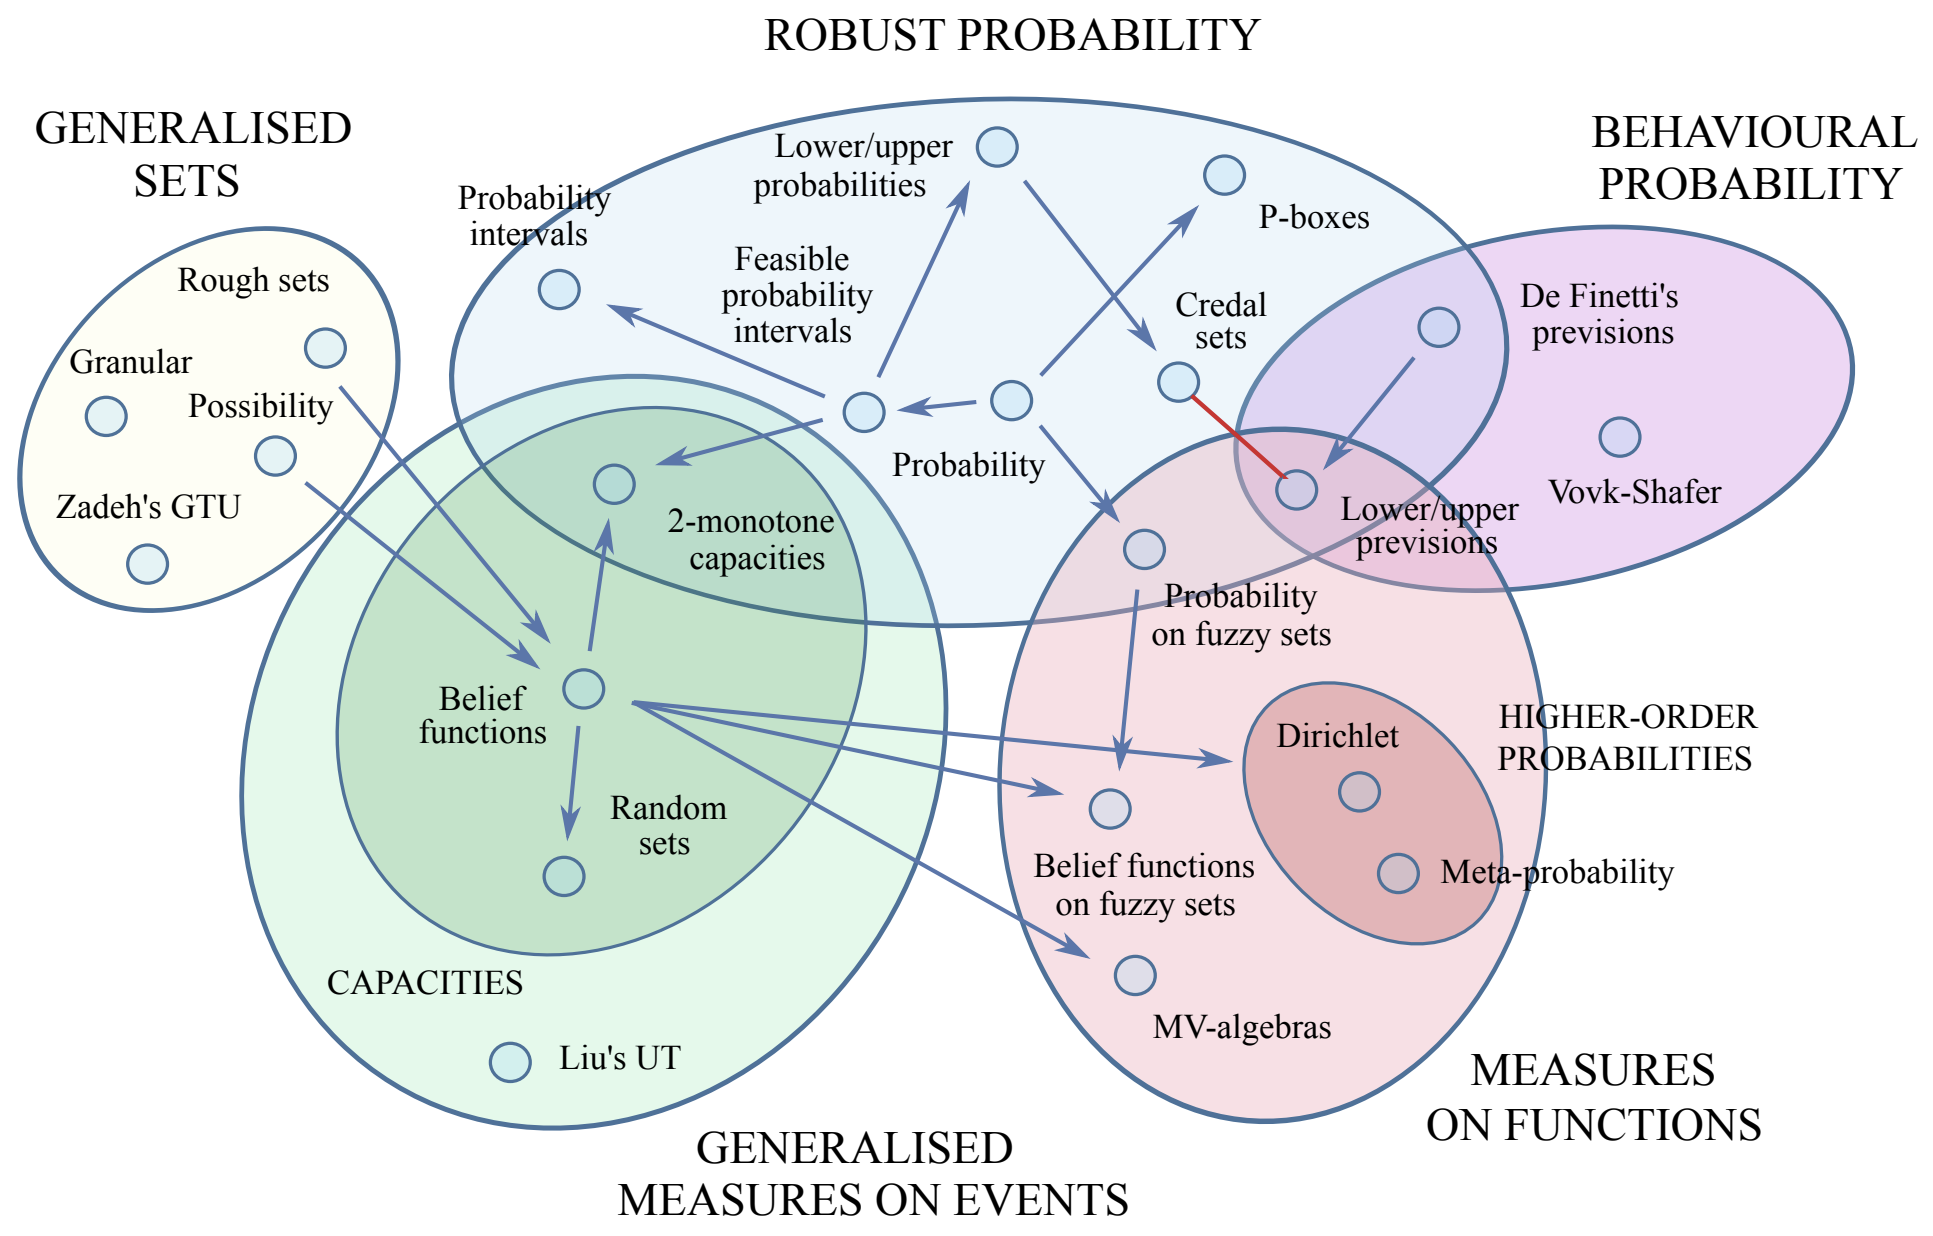
\includegraphics[width=\textwidth]{ch0/figures/Uncertainties Diagram.png}
    \caption{A classification of uncertainty theories showing their relationships and hierarchies. The theories are grouped based on their rationale and class of objects they attempt to mathematically model. Arrows indicate generalization relationships, pointing from more specific to more general frameworks. Extracted from \cite{uncertaintymeasuresbigpicture}.}
    \label{fig:uncertainty_taxonomy}
\end{figure}













































\section{Structure of this work}







\chapter{Fuzzy Set Theory}
This chapter draws upon foundational concepts and theoretical frameworks presented in \cite{FULLER1} and \cite{FULLER2}. 
% \section*{Motivation}
% Fuzzy sets were introduced by Zadeh in 1965 \cite{Zadeh1965}. 
% \signal{the example of tall people, we want to model imprecision and why probability theory is not well suited for this. También pensar si voy a diferenciar entre incertidumbre epistemológica o aleatoria, o si eso lo meto cuando hable de possibility.}

\section{Fuzzy Sets}
\signal{Decir cómo a partir de ese concepto de partial membership llegamos a esto y cómo es una generalización de boolean membership de classical sets. Di también que con classical y crisp nos referimos a boolean sets y con fuzzy a los otros. Di que usas la xi para la boolean membership y mu para la fuzzy en general}

\begin{definition}[Fuzzy Set]
    Let $X\neq\emptyset$ a set. Then we define a \textbf{fuzzy set A in X}, i.e., $A \in \fuzzy{X}$ as:
    \[A=\{(x,\mu_A(x))\mid x\in X\}\]
    Where $\mu_A:X\longrightarrow [0,1]$ is the \textbf{membership function} and $X$ is the \textbf{domain} of the fuzzy set.
\end{definition}

\begin{remark}
     Both the fuzzy set and the membership function uniquely identify each other.
\end{remark}

\begin{notation}{Notation}
    We may use \( A(x) \equiv \mu_A(x) \) interchangeably.
\end{notation}

\begin{definition}[Support]
    Let $A \in \fuzzy{X}$. The set of non zero membership value elements is called the support:
    \[\textnormal{Supp}(A)=\{x\in X \mid A(x)>0\}\]
\end{definition}

\signal{
\begin{definition}[Normal Fuzzy Set]
    A fuzzy set is called \textbf{normal} if there exists $x\in X$ such that $A(x)=1$. Otherwise it is called \textbf{subnormal}.
\end{definition}
}
\begin{definition}[$\alpha$-cut]
    Let $\alpha \in [0,1]$, the $\alpha$-cut (also called $\alpha$-cut) of a fuzzy set \( A \in \fuzzy{X}\) is:
    \[
    [A]^\alpha =
    \begin{cases}
    \{x \in X \mid A(x)\geq \alpha\} & \text{if } \alpha > 0, \\
    \textnormal{cl}(\textnormal{Supp}(A)) & \text{if } \alpha = 0.
    \end{cases}
    \]
    where \textit{cl} denotes the closure.
\end{definition}

\signal{
    \begin{definition}[Extremes of the support]
        
    \end{definition}
}


\begin{definition}[Fuzzy Subset]
    Given the fuzzy sets $A, B \in \fuzzy{X}$ we say $A$ is a fuzzy subset of $B$ (and write $A \subseteq B$) if and only if $A(x)
    \leq B(x) \forall x \in X$.

    Analogously, $A$ and $B$ are equal if and only if $A(x)=B(x) \forall x \in X$, i.e., each of them is a subset of the other.
\end{definition}

\begin{example}
    Here are some examples of common fuzzy sets:
    \begin{itemize}
        \item \textbf{Empty Fuzzy Set in $X$:} such that $\emptyset(x)=0 \forall x \in X$.
        \item \textbf{Universal Fuzzy Set in $X$:} such that $X(x)=1  \forall x \in X$.
        \item \textbf{Fuzzy Point in $X$:} such that $P(x_0)=1 \land A(x)=0 \forall x \in X-\{x_0\}$
        \item \textbf{Fuzzy Number:} Usually defined as a fuzzy set in $\mathbb{R}$ with some desirable properties. Will be covered in Section \ref{sec:fuzzy_numbers}.
    \end{itemize}
\end{example}

\section{Union, Intersection and Complement of Fuzzy Sets}
% \begin{notation}[label={not:OpsFS}]{Notation for variables in the current section}
%     In this section, we use the variable \( x \) to represent time and \( y \) to represent distance.
%   \end{notation}

The notions of union and intersection in fuzzy sets were first introduced by Zadeh \cite{Zadeh1965} using the operations $\max\{A(x),B(x)\}$ and $\min\{A(x),B(x)\}$ respectively. These can be intuitively interpreted as follows: the union is the \textit{smallest} fuzzy set (having lowest membership values) that contains both sets, while the intersection is the \textit{biggest} fuzzy set (having highest membership values) that is contained by both sets.\\

However, these operations can be generalized by two broader classes of operators: triangular norms (for intersection) and triangular conorms (for union).

Triangular norms were first introduced by Karl Menger in 1942 \cite{OriginTNorms} in the context of probabilistic metric spaces. When generalizing distances between points to probability distributions (representing the probability that the distance is less than or equal to a given value), Menger defined an operation $T:\,[0,1]\times [0,1]\to [0,1]$ to preserve the triangular inequality. For points $x,y,z$ in a metric space with distance function $d(\cdot,\cdot)$, this operation satisfies:

\begin{equation}\label{eq:Ftriangle_inequality}
d(x, z) \leq d(x, y) + d(y, z) \quad \longrightarrow \quad F_{xz}(t + s) \geq T(F_{xy}(t), F_{yz}(s)) \quad \forall t,s \geq 0
\end{equation}

This inequality means that the probability of $d(x,z)$ being less than $t+s$ must be at least the t-norm of the probabilities that $d(x,y)<t$ and $d(y,z)<s$. Note the change from $\leq$ to $\geq$ in the inequality. This is consistent with \textit{larger} probabilities indicating \textit{smaller} distances are more likely.\\

Since this originated in the context of distances, the following properties were required for an operator to be a t-norm\footnote{Associativity and one identity were not originally proposed by Menger but were later added by Sklar and Schweizer \cite{Sklar1983} in their refinement of triangular norms}:

\begin{itemize}
  \item \textbf{Symmetry:} The order of combining probabilities shouldn't matter, just as intersection of sets is commutative. That is, combining probabilities for distances $(x,y)$ and $(y,z)$ should give the same result regardless of order.
  
  \item \textbf{Associativity:} When combining multiple probabilities (e.g., for paths through points $x,y,z,w$), the grouping shouldn't affect the result. This extends the triangular norm to be consistent with polygonal inequalities, similar to how nested intersections satisfy $(A \cap B) \cap C = A \cap (B \cap C)$.
  
  \item \textbf{Monotonicity:} If the probability $F_{xy}(t)$ increases, then the lower bound for $F_{xz}(t+s)$ given by $T(F_{xy}(t), F_{yz}(s))$ should not decrease. This is analogous to how adding elements in crisp sets (or increasing membership degrees in fuzzy sets) cannot reduce the intersection set.
  
  \item \textbf{One Identity:} If $F_{yz}(s) = 1$ (meaning $d(y,z) < s$ with certainty), then $F_{xz}(t+s)$ depends only on $F_{xy}(t)$. This is analogous to how intersecting with the universal set preserves the original set.
\end{itemize}


% \say{The name \textit{triangular norm} refers to the fact that in the framework of probabilistic metric spaces, t-norms and t-conorms are used to generalize triangle inequality of ordinary metric spaces.}\cite{NGAN2018}\\

Therefore, the concept of intersection (conjunction) of fuzzy sets is generally represented by a triangular norm (also called a t-norm).

\begin{definition}[Triangular Norm]
    A mapping $T:[0,1]\times [0,1] \longrightarrow [0,1]$ that satisfies:
    \begin{romanenum}
      \item \textbf{Symmetricity:} $T(x,y) = T(y,x) \quad \oldforall x,y \in [0,1]$
      \item \textbf{Associativity:} $T(x,T(y,z)) = T(T(x,y),z) \quad \oldforall x,y,z \in [0,1]$
      \item \textbf{Monotonicity:} $T(x,y) \leq T(x',y') \quad \textnormal{if }x\leq x' \textnormal{ and } y\leq y' \quad \oldforall x,y,x',y' \in [0,1]$
      \item \textbf{One Identity:} $T(x,1) = T(1,x) = x \quad \oldforall x \in [0,1]$
    \end{romanenum}
    is called a triangular norm or t-norm. Defines the \textbf{intersection} of two fuzzy sets $A$ and $B$ on $X$ by giving the membership function as $(A \cap B) (x) = T(A(x),B(x)) \forall x \in X$ 
\end{definition}

Its dual operator can also be obtained by a similar reasoning as before, but instead of considering the probability distribution of finding both points closer than a given distance, it considers the probability distribution ($G_{uv}(t) = 1 - F_{uv}(t)$) of finding them further apart than that distance. In this case, both inequalities are $\leq$ since larger probabilities indicate that greater distances are more likely.
\begin{equation}\label{eq:Gtriangle_inequality}
d(x, z) \leq d(x, y) + d(y, z) \quad \longrightarrow \quad G_{xz}(t + s) \leq S(G_{xy}(t), G_{yz}(s))
\end{equation}

The reasoning regarding the properties is entirely analogous to the previous case, with the only difference being that $F_{uv}(t) = 1 \Leftrightarrow  G_{uv}(t) = 0$, and here the identity element is zero (union with the empty set).



\begin{definition}[Triangular Conorm]
  A mapping $S:[0,1]\times [0,1] \longrightarrow [0,1]$ that satisfies:
  \begin{enumerate}[(i)]\setlength{\itemindent}{2em}
    \item \textbf{Symmetricity:} $S(x,y) = S(y,x) \quad \oldforall x,y \in [0,1]$
    \item \textbf{Associativity:} $S(x,S(y,z)) = S(S(x,y),z) \quad \oldforall x,y,z \in [0,1]$
    \item \textbf{Monotonicity:} $S(x,y) \leq S(x',y') \quad \textnormal{if }x\leq x' \textnormal{ and } y\leq y' \quad \oldforall x,y,x',y' \in [0,1]$
    \item \textbf{Zero Identity:} $S(x,0) = S(0,x) = x \quad \oldforall x \in [0,1]$
  \end{enumerate}
  is called a triangular conorm or t-conorm. Defines the \textbf{union} of two fuzzy sets $A$ and $B$ on $X$ by giving the membership function as $(A \cup  B) (x) = S(A(x),B(x)) \forall x \in X$ 
    
\end{definition}

Complement was defined by Zadeh \cite{Zadeh1965} as\footnote{This is not the only definition that satisfies the axioms of a complement and is compatible with the classical limit, but it is the simplest one and will be used in this text. Other alternatives and their axioms can be found in \cite{Sladoje2007}. In \cite{Klement2000}, this is called the standard negation $N_s$.}:

\begin{definition}[Complement]
  The complement of a fuzzy set $A\in \fuzzy{X}$ is another fuzzy set with membership function given by $\overline{A}(x) \coleq 1 - A(x) \forall x\in X$
\end{definition}

Notice that this definition of complement is consistent with the classical definition of complement but implies that an element might have \textbf{non-zero partial membership} to both a fuzzy set and its complement: Let $A$ be a fuzzy set on $X$ and $x \in X / A(x)\notin \{0,1\}$ then $\overline{ A}(x)= 1 - A(x) \notin \{0,1\}$.\\

One consequence of this fact is that the union of a fuzzy set and its complement is not the total set in general. Analogously, the intersection will not the empty set in general. Those two properties that hold in classical sets but might not be true in fuzzy sets, are often called the \textbf{laws of excluded middle and of non-contradiction}, respectively.\\

However, there are t-norms and t-conorms such as the ones named after \luka that do satisfy both laws\footnote{Indeed, all continuous t-norms in agreement with non-contradiction are isomorphic to \luka \cite[p.~7]{LukasiewiczNonContrad}.}. Another example is the drastic t-norm which also satisfies the law of non-contradiction, but not the law of excluded middle. See example \ref{ex:basic_tnorms} for their formal expressions. \signal{All of this, has implications for the derived logic that will be explained in section \ref{sec:fuzzy_logic}. }\\

Another important property that classical union and intersection satisfy is De Morgan's Laws. For an arbitrary pair of t-norm and t-conorm, these laws are not automatically satisfied. However, there are specific pairs that do fulfill them. To illustrate the relationship between t-norms and t-conorms that satisfy De Morgan's Laws, we can use our probabilistic metric space analogy. Reconsidering the probabilistic metrics $F,G$ introduced earlier and substituting $F = 1 - G$ into equation \ref{eq:Ftriangle_inequality}, we obtain:

\[ G_{xz}(t + s) \leq 1 - T(1 - G_{xy}(t), 1 - G_{yz}(s))\]

Comparing this with equation \ref{eq:Gtriangle_inequality}, we can derive a relationship between t-norms and t-conorms\footnote{The relation from proposition \ref{prop:rel_tnorm_tconorm} directly mirrors the classical set union definition via intersection and negation ($A\cup B \coleq \neg (\neg A \cap \neg B)$), which can be visualized with a Venn diagram. Therefore, it is natural that this condition is equivalent to the De Morgan's Laws.}, which is formalized in the following proposition:

\begin{proposition}[Relationship between t-norm and t-conorm]\label{prop:rel_tnorm_tconorm}
  Given a t-norm $T$, the t-conorm is $S(a,b)\coleq 1 - T(1-a, 1-b)$ if and only if the union and intersection defined by that pair satisfy the De Morgan's Laws.
\end{proposition}
\begin{remark}
  It is easy to see that the previous relation is equivalent to $T(a,b) = 1-S(1-a, 1-b)$ which can be obtained simply by substituting $a'=1-a$ and $b'=1-b$, i.e., working with the complementary fuzzy sets.
\end{remark}

\begin{proof}
  Let $x\in X$, $A$, $B$ be fuzzy sets over $X$ with $a \coleq A(x)$ and $b \coleq B(x)$\\

  $\quad \boxed{\text{not}(A \text{ or } B) = (\text{not } A) \text{ and } (\text{not } B)}$\\
  [0.5em]
  $\overline{ S(a,b)} = T(\overline{ a}, \overline{ b}) \iff 1 - S(a,b) = T(1-a, 1-b) \iff S(a,b) = 1 - T(1-a, 1-b)$\\

  $\quad \boxed{\text{not}(A \text{ and } B) = (\text{not } A) \text{ or } (\text{not } B)}$\\
  [0.5em]
  $\overline{ T(a,b)} = S(\overline{ a}, \overline{ b}) \iff 1 - T(a,b) = S(1-a, 1-b) \iff T(a,b) = 1 - S(1-a, 1-b)$

\end{proof}

\signal{Creo que además de esto de las leyes de de Morgan, también nos da que el modus ponen funciona si se cumple la propiedad esa. Además no sé si se llama residual property.}

\signal{
  Lo de Archimedean sirve para el teorema 1.8.1 de \cite{FULLER2}. Y tb con la law of large numbers con LR-fuzzy numbers.}

  \signal{Strict T-norms iff satisfy conditional cancellation}

  \signal{Tambien lo de que la T-norm e distributiva con max/sup sirve para justificar la definicion del producto cartesiano, así que esa propiedad la tendré que meter por aquí igual.}


The following algebraic properties will be needed when defining fuzzy logics and to classify continuous t-norms \cite[Def.~2.1 \& 2.13]{Klement2000}:

\begin{definition}[Nilpotent Element and Nilpotent T-norm]
Let $T$ be a t-norm. An element $a \in ]0,1[$ is a \emph{nilpotent element} of $T$ if there exists $n \in \mathbb{N}$ such that $a_T^{(n)} = 0$, where $a_T^{(n)} = T(a, a_T^{(n-1)})$ with $a_T^{(1)}=a$.

A t-norm is called nilpotent if and only if it is continuous and every $a\in ]0,1[$ is nilpotent.
\end{definition}

\begin{definition}[Strict T-norm]
  A t-norm is called strict if it is continuous and strictly monotone.
\end{definition}


\begin{definition}[Zero Divisor]
Let $T$ be a t-norm. An element $a \in ]0,1[$ is a \emph{zero divisor} of $T$ if there exists $b \in ]0,1[$ such that $T(a,b)=0$.
\end{definition}

\begin{definition}[Idempotent Element]
  Let $T$ be a t-norm. An element $a \in [0,1]$ is an \emph{idempotent element} of $T$ if $T(a,a)=a$. The elements $0$ and $1$ are always trivial idempotent elements.
  \end{definition}
  

\begin{definition}[Archimedean T-norm]
A t-norm $T$ is \emph{Archimedean} if for each $(x,y) \in ]0,1[^2$ there is an $n \in \mathbb{N}$ with $x_T^{(n)} < y$. \cite[Def.~2.9]{Klement2000}  

In particular, a \textit{continuous} t-norm $T$ is Archimedean if and only if $T(x,x) < x \forall x \in ]0,1[$, i.e. it doesn't have non-trivial idempotent elements. \cite[Thm.~2.12]{Klement2000}
\end{definition}


When a t-norm is continuous and Archimedean, there's a crucial relationship between its algebraic properties. It cannot be simultaneously strict and possess nilpotent elements (or zero divisors):

\begin{theorem}{Algebraic properties of continuous Archimedean T-norms \cite[Thm.~2.18]{Klement2000}}\label{thm:alg_arch_cont}
Let $T$ be a continuous Archimedean t-norm. Then the following are equivalent:
\begin{romanenum}
    \item $T$ is \emph{nilpotent}.
    \item There exists some nilpotent element of $T$.
    \item There exists some zero divisor of $T$.
    \item $T$ is not \emph{strict}.
\end{romanenum}
\end{theorem}

% \begin{remark}\label{rem:split_tnorms}
%   Continuous Archimedean t-norms can be splitted into two classes according to their nilpotent elements \cite[Cor.~3.30]{Klement2000}: strict (having no nilpotent elements except $0$) and nilpotent (where every element in $]0,1[$ is nilpotent).
% \end{remark}


  \begin{example}[Basic T-norms {\cite[Ex.~1.2]{Klement2000}}]\label{ex:basic_tnorms}
    These four t-norms are canonical examples because they represent the extremal and most representative cases with respect to the order relation (see definition \ref{def:weaker}) and algebraic properties. From weaker to stronger they are: $T_D \leq T_L \leq T_P \leq T_M$. 
    
    All of them are plotted in figures \ref{fig:2D_tnorms} and \ref{fig:tnorms_3D_plots}.
      \begin{itemize}
        \item \textbf{Minimum ($T_M$):} 
            This is the strongest t-norm (\cite[Rem.~1.5(i)]{Klement2000}). Every element is idempotent (indeed it is the only t-norm satisfying that \cite[Lem.~1.2.3]{FULLER2} \signal{igual este paréntesis debería escribirlo como un resultado mejor}), therefore it is not Archimedean. It has no zero divisors and no nilpotent elements other than 0.
    
        \[T_M(x, y) = \min(x, y) \quad S_M(x, y) = \max(x, y)
    \]
        \item \textbf{Product ($T_P$):} 
        This t-norm is strict Archimedean (\cite[Ex.~2.14(i)]{Klement2000}). It has only $0$ and $1$ as idempotent elements, no nilpotent elements (other than $0$), and no zero divisors (\cite[Ex.~2.2(i)]{Klement2000}).
        \[T_P(x, y) = x \cdot y \quad S_P(x, y) = x + y - x \cdot y\]
        \item \textbf{Łukasiewicz ($T_L$):} 
        This t-norm is nilpotent Archimedean (\cite[Ex.~2.14(i)]{Klement2000}). It has only $0$ and $1$ as idempotent elements. Every $a \in ]0,1[$ is a nilpotent element and also a zero divisor (\cite[Ex.~2.2(i)]{Klement2000}).
        \[T_L(x, y) = \max(0, x + y - 1) \quad S_L(x, y) = \min(1, x + y)\]
        \item \textbf{Drastic Product ($T_D$):} This is the weakest t-norm (\cite[Rem.~1.5(i)]{Klement2000}). It is Archimedean since $T_D(x,x)=0 < x$ for $x \in ]0,1[$. It has only $0$ and $1$ as idempotent elements. Every $a \in ]0,1[$ is a zero divisor, and also nilpotent (since $a_D^{(2)} = T_D(a, T_D(a,a)) = T_D(a,0) = 0$ for $a<1$). It is not continuous.
        \[T_D(x, y) = \begin{cases} \min(x,y) & \text{if } \max(x,y)=1 \\ 0 & \text{otherwise} \end{cases} \quad S_D(x, y) = \begin{cases} \max(x,y) & \text{if } \min(x,y)=0 \\ 1 & \text{otherwise} \end{cases}\]
      \end{itemize}
    \end{example}


\begin{figure}[ht]
    \centering
    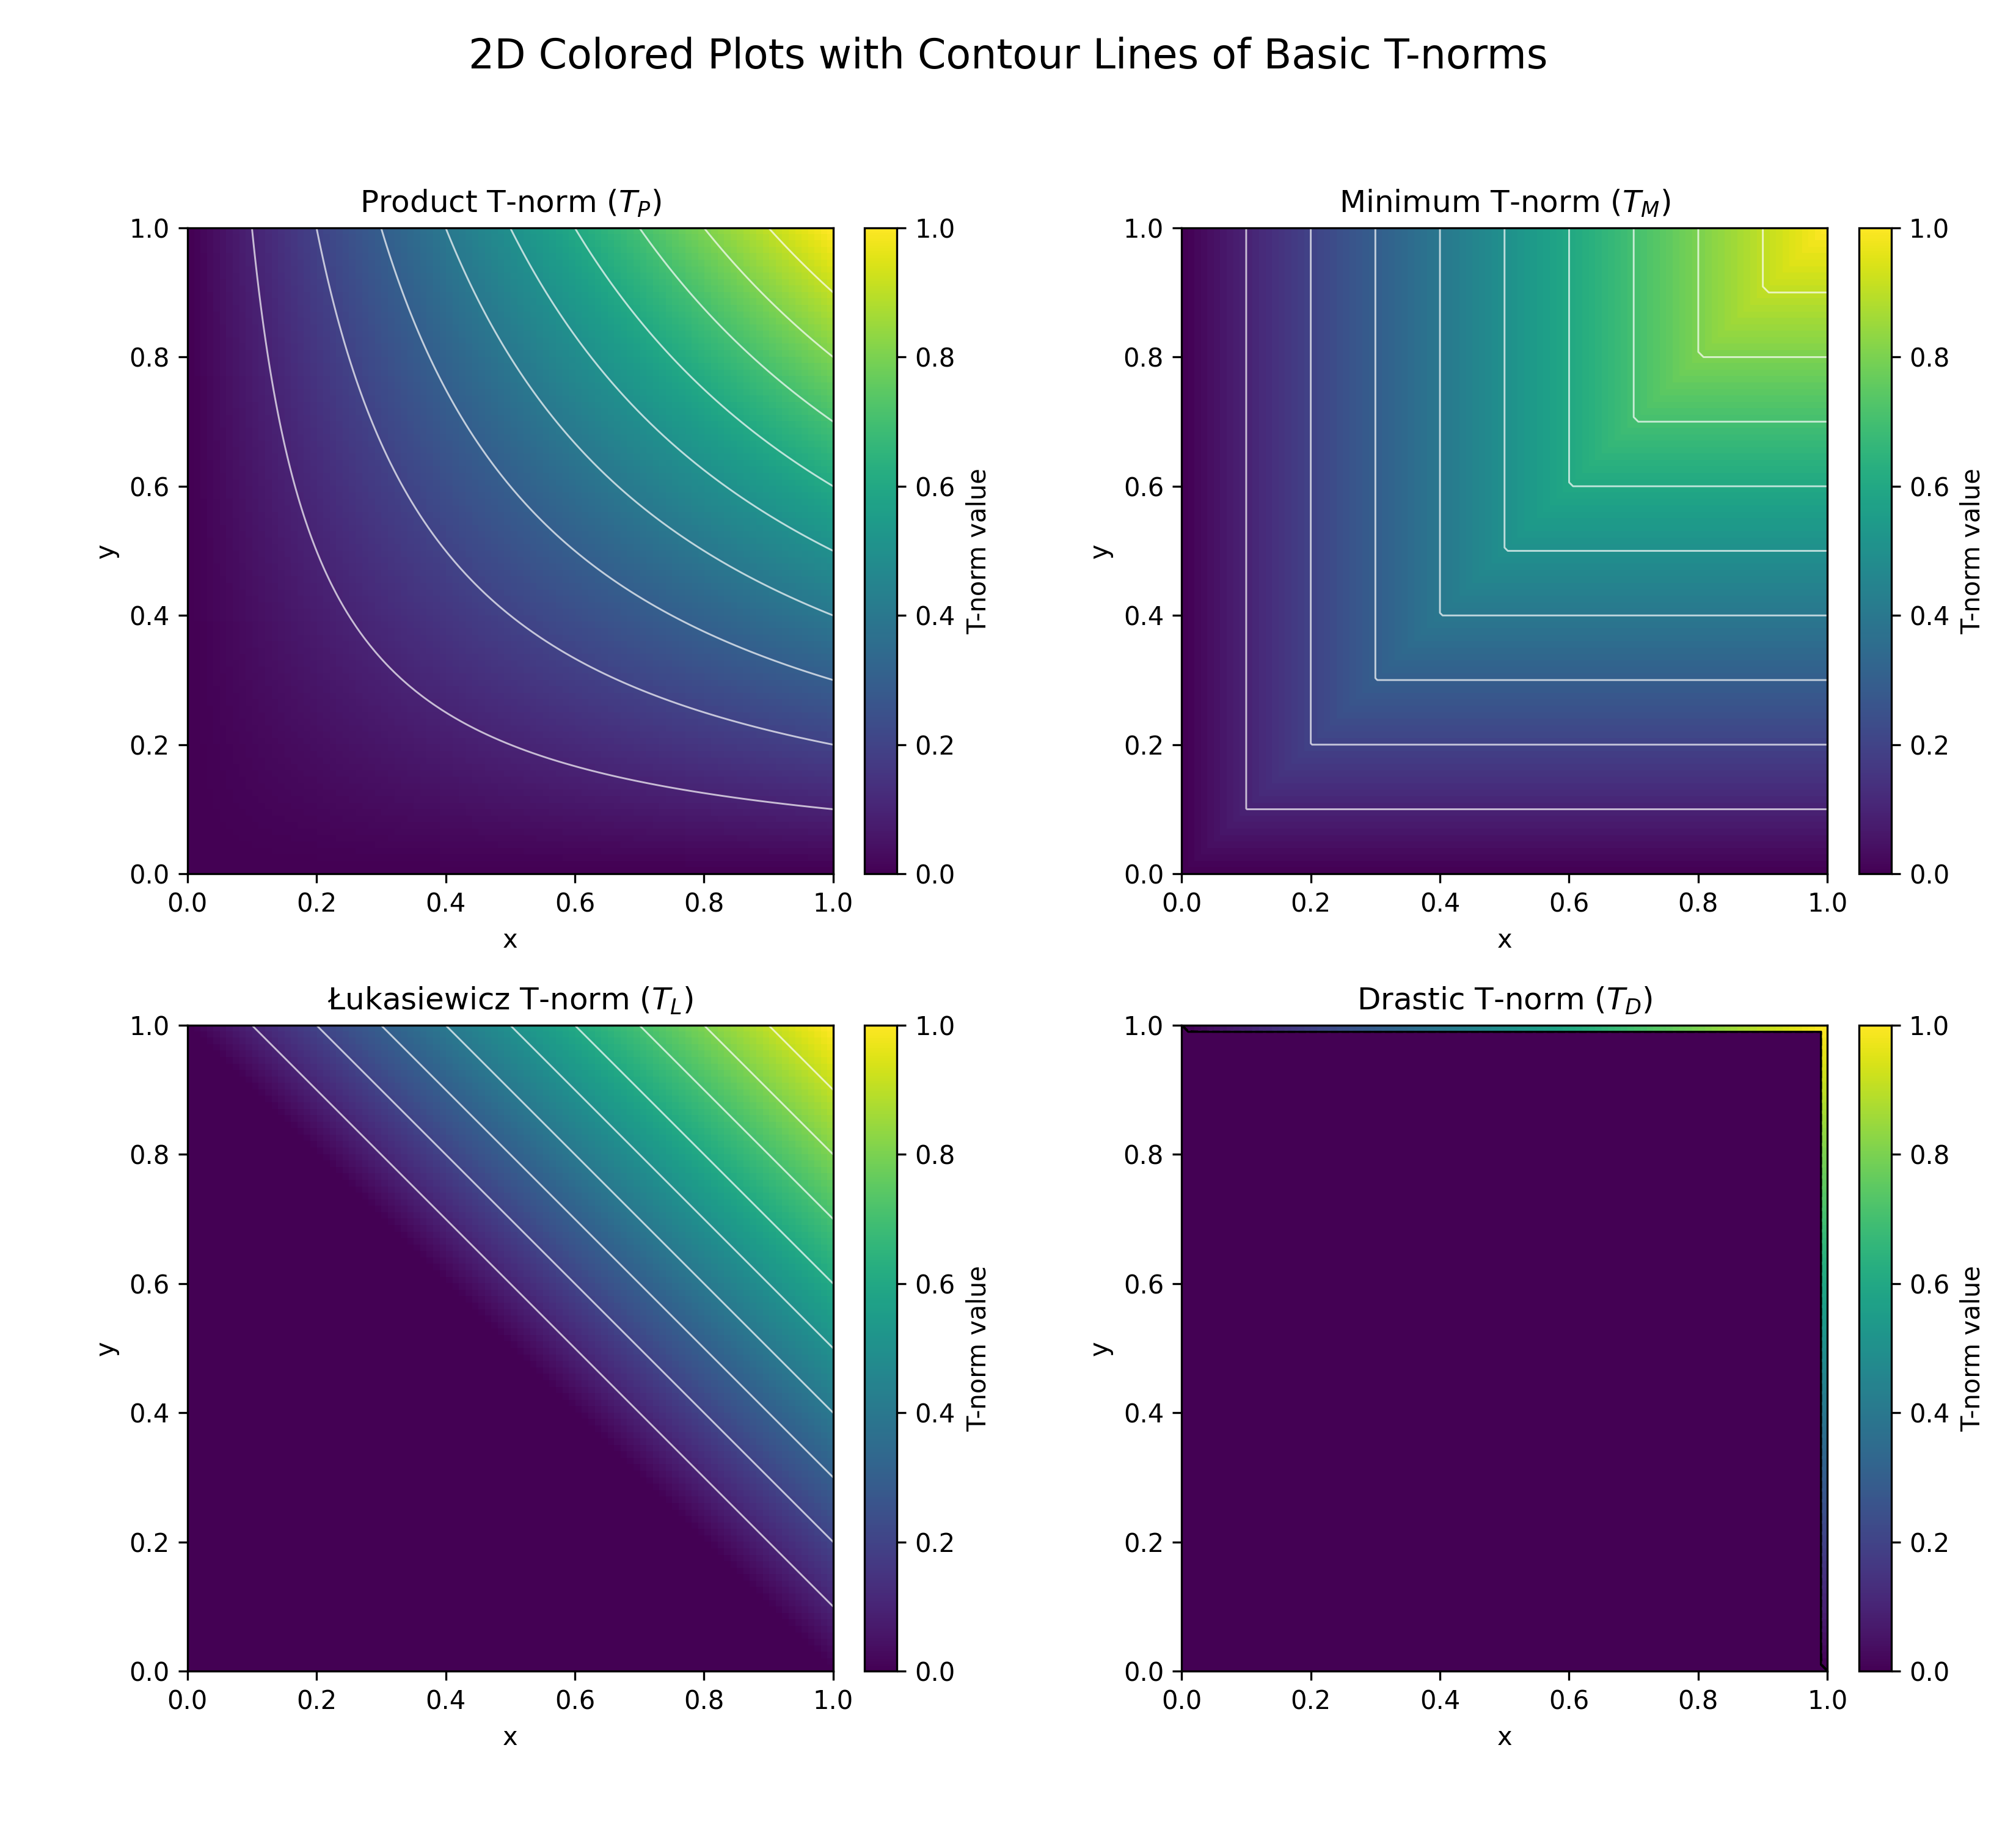
\includegraphics[width=0.85\textwidth]{ch1/figures/tnorms_2D_plots.png}
    \caption{Level curves of basic t-norms ($T_M$, $T_P$, $T_L$, $T_D$) in the unit square $[0,1]^2$. The different shapes of the white level curves illustrate the distinct behaviors and algebraic properties of each t-norm.}
    \label{fig:2D_tnorms}
\end{figure}


\begin{figure}[!ht]
    \centering
    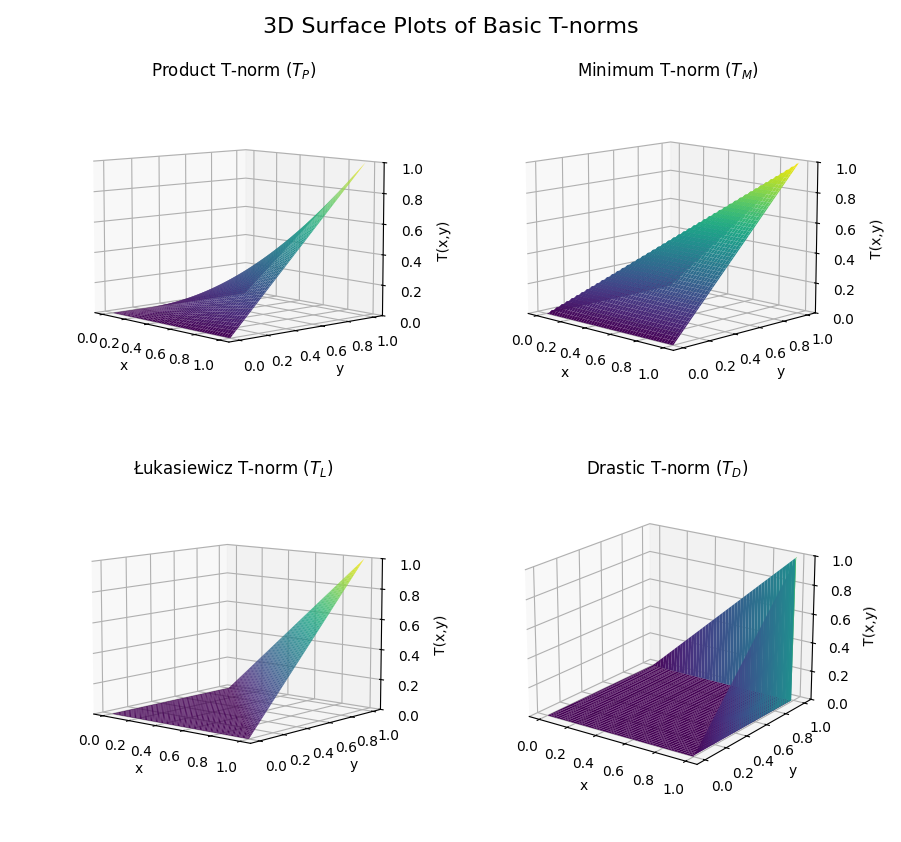
\includegraphics[width=0.95\textwidth]{ch1/figures/tnorms_3D_plots.png}
    \caption{3D surface plots of the basic t-norms ($T_M$, $T_P$, $T_L$, $T_D$) over the unit square $[0,1]^2$. The minimum t-norm forms a sharp ridge along $x=y$, the product t-norm is smoothly curved, the Łukasiewicz t-norm is planar except for a triangular region where it is zero, and the drastic t-norm is flat except for the edges. All of them are identical at the boundaries of the unit square.}
    \label{fig:tnorms_3D_plots}
\end{figure}


\subsection{Classification of T-norms}\label{sec:class_tnorms}
The first and most straight forward way to classify them is by defining the following partial order on the set of all t-norms. 
\begin{definition}[Weaker/Stronger t-norm {\cite[Def.~1.4]{Klement2000}}]\label{def:weaker}
  Given two t-norms $T_1$ and $T_2$, $T_1$ is said to be \emph{weaker} than $T_2$ (denoted $T_1 \leq T_2$) if $T_1(x,y) \leq T_2(x,y) \forall x,y \in [0,1]$.
  Equivalently, $T_2$ is said to be \emph{stronger} than $T_1$.
\end{definition}

\begin{remark}
  It's a fundamental result that for any t-norm $T$, we have $T_D \leq T \leq T_M$, where $T_D$ and $T_M$ are the drastic and the minimum t-norms respectively (\cite[Rem.~1.5]{Klement2000}).
\end{remark}

The interpretation is that a weaker t-norm can be seen as a stricter and more pessimistic intersection (conjunction in the fuzzy logic derived), returning lower membership values than a stronger one. Notice that it is not a total order: there are pairs of t-norms where none of them is weaker than the other. Some examples, such as the product $T_P$ and Yager $T_2^Y$ (see \ref{ex:families_tnorms} for the definition of the Yager family) t-norms, are shown in \cite[Fig.~6.1]{Klement2000}.\\


Another way to classify t-norms is based on their continuity properties. Continuous t-norms can be divided into two main classes (Fig.~\ref{fig:tnorm_classification}): Archimedean and non-Archimedean t-norms. The Archimedean t-norms can be further subdivided into strict and nilpotent t-norms (using the theorem \ref{thm:alg_arch_cont})\footnote{This classification is also characterized by the behavior of their generator functions at 0. For a more detailed discussion and definitions related to generators, see Appendix \ref{app:generators_tnorms}}:

\begin{itemize}
    \item $T$ is \textbf{strict} if it doesn't have any nilpotent elements except $0$. This means $T(x,y)>0$ whenever $x,y > 0$. (\cite[Cor.~3.30(i)]{Klement2000}).
    \item $T$ is \textbf{nilpotent} if every element in $]0,1[$ is nilpotent. This implies that for any $x,y \in ]0,1[$, there exists $n$ such that $T(x, \dots, x)$ ($n$ times) is $0$. (\cite[Cor.~3.30(ii)]{Klement2000}).
\end{itemize}


\begin{figure}[ht]
\centering
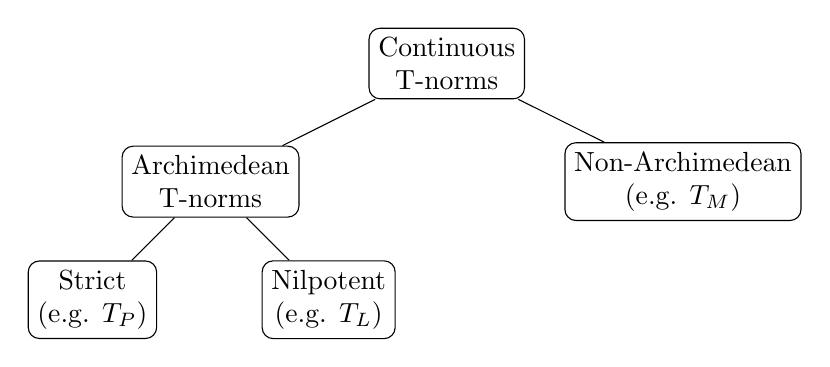
\begin{tikzpicture}[
    level 1/.style={sibling distance=60mm},
    level 2/.style={sibling distance=30mm},
    every node/.style={draw,rounded corners,align=center}
]
\node {Continuous\\ T-norms}
    child {
        node {Archimedean\\ T-norms}
        child {
            node {Strict\\ (e.g. $T_P$)}
        }
        child {
            node {Nilpotent\\ (e.g. $T_L$)}
        }
    }
    child {
        node {Non-Archimedean\\ (e.g. $T_M$)}
    };
\end{tikzpicture}
\caption{Classification of continuous t-norms}
\label{fig:tnorm_classification}
\end{figure}



Indeed, strict and nilpotent t-norms form two classes that are closed under certain isomorphic transformations: 

\begin{definition}[Isomorphic T-norms {\cite[Prop.~2.28(iv)]{Klement2000}}]
  Two t-norms $T_1$ and $T_2$ are \emph{isomorphic} if there exists a strictly increasing bijection $\varphi: [0,1] \to [0,1]$ (an automorphism of the unit interval) such that $T_2(x,y) = \varphi^{-1}(T_1(\varphi(x), \varphi(y)))$ for all $x,y \in [0,1]$.
\end{definition}
This definition is completely analogous for t-conorms. The isomorphism can be understood as a rescaling of the unit interval. The original t-norm is applied to this scaled domain and then the scale is reverted to make the output comparable to the original inputs $x,y$ (otherwise, the one identity property might not hold). Isomorphic t-norms share the same algebraic structure, merely operating on rescaled inputs and outputs via $\varphi$. A fundamental result is that (up to isomorphism) there are only two distinct types of continuous Archimedean t-norms: the product type and the Łukasiewicz type.
\begin{proposition}[{Classes of continuous Archimedean t-norms \cite[Cor.~5.7]{Klement2000}}]
  {\color{white}.}
  \begin{enumerate} 
      \item Every strict t-norm is isomorphic to the Product t-norm $T_P$.
      \item Every nilpotent t-norm is isomorphic to the Łukasiewicz t-norm $T_L$.
  \end{enumerate}
\end{proposition}

For general continuous t-norms that are not Archimedean, there must be non-trivial idempotent elements. These are constructed using ordinal sums.
\begin{definition}[Ordinal Sum of T-norms {\cite[Def.~3.44]{Klement2000}}]
Let $(T_\alpha)_{\alpha \in A}$ be a family of t-norms and $(]a_\alpha, e_\alpha[)_{\alpha \in A}$ be a family of non-empty, pairwise disjoint open subintervals of $[0,1]$. The t-norm $T$ defined by
\[
T(x,y) =
\begin{cases}
  a_\alpha + (e_\alpha - a_\alpha) \cdot T_\alpha \left( \frac{x-a_\alpha}{e_\alpha - a_\alpha}, \frac{y-a_\alpha}{e_\alpha - a_\alpha} \right) & \text{if } (x,y) \in [a_\alpha, e_\alpha]^2 \text{ for some } \alpha \in A \\
  \min(x,y) & \text{otherwise}
\end{cases}
\]
is called the \emph{ordinal sum} of the summands $(a_\alpha, e_\alpha, T_\alpha)$, $\alpha \in A$.
\end{definition}
Intuitively (see figure \ref{fig:ordinal_sum_tnorm}), an ordinal sum constructs a t-norm by combining scaled copies of other t-norms on the unit square $[0,1]^2$. For each interval $]a_\alpha, e_\alpha[$ along the main diagonal, a t-norm $T_\alpha$ operates within the square region $[a_\alpha, e_\alpha]^2$. Inside these "active" regions, inputs are first scaled down from $[a_\alpha, e_\alpha]$ to $[0,1]$ via linear transformations, then $T_\alpha$ is applied, and finally the result is scaled back to $[a_\alpha, e_\alpha]$. Outside these regions, the t-norm defaults to the minimum $T_M$, which ensures continuity (if the $T_\alpha$ are continuous) and makes the interval endpoints $a_\alpha, e_\alpha$ into idempotent elements of the resulting t-norm. This continuity at the boundaries of the active region is possible because any t-norm $T$ coincides with $T_M$ along the border of any square region centered in the diagonal $(x,x)$.\\

\begin{figure}[!ht]
    \centering
    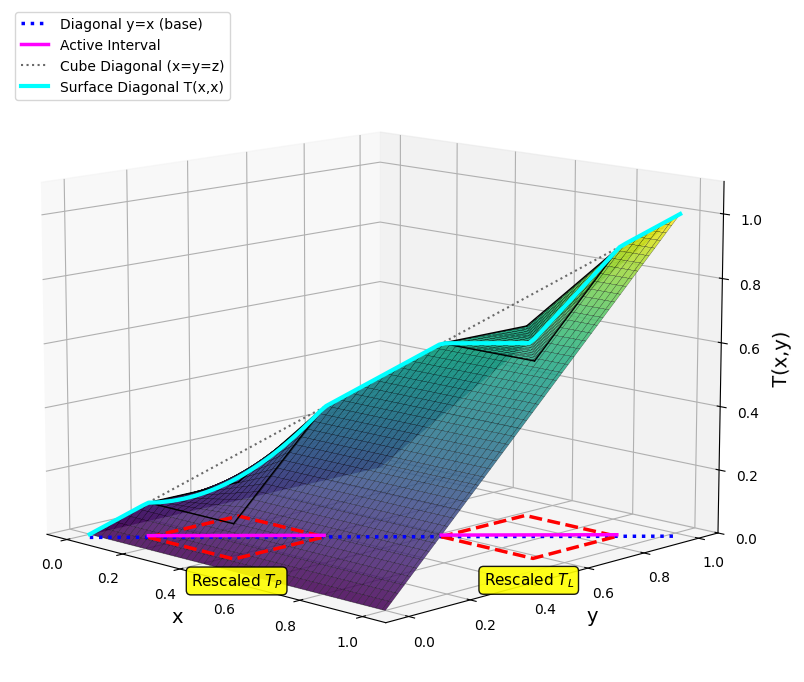
\includegraphics[width=0.9\textwidth]{ch1/figures/ordinal_sums.png}
    \caption{Visualization of an ordinal sum of t-norms. Each colored square (black on the surface, red on the xy plane) along the diagonal corresponds to an "active" region where a rescaled t-norm (Product or Łukasiewicz) operates. Outside these regions, the minimum t-norm $T_M$ is used. It is inspired by \cite[Fig.~3.16]{Klement2000}}
    \label{fig:ordinal_sum_tnorm}
\end{figure}



\begin{theorem}[Representation of Continuous T-norms {\cite[Thm.~5.11]{Klement2000}}]
  A function $T: [0,1]^2 \to [0,1]$ is a continuous t-norm if and only if $T$ is uniquely representable as an ordinal sum of continuous Archimedean t-norms.
\end{theorem}

The main idea behind this representation is leveraging the idempotent elements in the diagonal. Start with all the diagonal being idempotent (only possibility is $T_M$), and remove all the non-idempotent intervals (where the t-norm is locally Archimedean) with one of the two possibilities in the continuous case: strict (isomorphic to $T_P$) or nilpotent (isomorphic to $T_L$).

\begin{remark}
  If the family of subintervals is empty, the ordinal sum is defined as $T_M$.
\end{remark}

Unlike continuous t-norms, non-continuous t-norms generally lack a unifying framework based on generator functions that allows for a similar classification. Their analysis, therefore, focuses on the particular (semi-)continuity and algebraic characteristics. For examples and a discussion on semi-continuity of t-norms, see appendix \ref{app:cont_tnorms} and \ref{app:semicont-tnorms}.











































\section{Fuzzy Relations}
  In the previous sections we have been working with a single domain denoted by $X$. Intuitively, it might be useful to think about the domain as the different values of a property (independently of the object that has that property). For example, we could say that for the property \textit{lenght} the domain is $\R^+\coleq
  \{x\in\R \mid x \geq 0\}$ and a person might have a \textit{height} defined in that domain (modeled as a fuzzy set), although not all length values will be compatible with a person's height since it is safe to assume impossible to be 10 meters tall, but we do not know where to place a sharp boundary, so the feasible region of heights is best represented by a fuzzy set. If we were to look at the arm length, then we would have another set of feasible lenghts. Treating each set independently, doesn't allow to distinguish between the people of the same height with different arm lenght or viceversa. Therefore it is needed to a way to differentiate each unique combination of attributes. Notice that in this example, height and arm length have the same domain but for example hair color would have a different domain.\\

  Mathematically, this is done with relations which are subsets of the cartesian product of the domains, so that each element is a unique possible combination of attributes, an ordered n-tuple. For simplicity, let us consider just the cartesian product of 2 sets since the general case can be obtained inductively (see remark below). Again, the ``fuzzy" part will be referred to how we generalize the membership values to the continuum.


  \begin{definition}[Fuzzy Relation]
    Let $X\neq \emptyset \neq Y$ be classical sets. Then a fuzzy relation $R$ is a fuzzy set on $X\times Y$, i.e., $R\in \fuzzy{X\times Y}$. $R(x,y)$ will denote the degree of membership of $(x,y) \in R$.
  \end{definition}

  \begin{notation}[label={not:compositionFS}]{Notation}
    Although Fuzzy Relations are Fuzzy Sets as well, the name distinction will be used to denote whether the domain is a cartesian product or not.
  \end{notation}

  \begin{remark}
    To formally extend the Cartesian product from two sets to \( n \) sets using induction, it is important to observe that it satisfies associativity up to a natural isomorphism, i.e., 
    \[
    (A\times B)\times C \cong A\times (B\times C).
    \]
    and that t-norms satisfy the associativity property.
  \end{remark}

  Before giving the definition of the fuzzy cartesian product, we need to first understand what the classical cartesian product is in terms of the membership function. When we define a cartesian product $A\times B$ as "\textit{all unique ordered pairs of elements from $A$ \textbf{and} $B$}", in terms of membership functions we are taking the intersection of membership to $A$ and membership to $B$. Therefore, generalizing that notion with a t-norm we get the following definition.

  \begin{definition}[Fuzzy Cartesian Product]
    It is a fuzzy relation $A\times B \in \fuzzy{X\times Y}$ such that the membership function is given by:
    \[ 
    (A\times B)(x,y) = T(A(x), B(y)), \quad \forall (x,y) \in X\times Y
    \]
    where $T$ is a t-norm.
  \end{definition}

  To justify the definition of the membership function of a cartesian product of two fuzzy sets, let us first recall that in classical sets, we can retrieve the orginal subsets individually by taking the projection of the cartesian product. Given $R$ a relation on $X\times Y$ the projections are:

  \[\Pi_X(R)=\{x \in X \mid \exists y \in Y \textnormal{ such that } (x,y) \in R\}\]
  \[\Pi_Y(R)=\{y \in Y \mid \exists x \in X \textnormal{ such that } (x,y) \in R\}\]

  Then, with the boolean membership, it can be expressed as well as:

  \[\Pi_X(R)(x)=\sup\{R(x,y) \mid y\in Y\}=
  \begin{cases}
    1 & \textnormal{if } \exists y \in Y \textnormal{ such that } (x,y) \in R \\
    0 & \textnormal{otherwise}
  \end{cases}
  \]
  \[
    \Pi_Y(R)(y)=\sup\{R(x,y) \mid x\in X\}=
    \begin{cases}
      1 & \textnormal{if } \exists x \in X \textnormal{ such that } (x,y) \in R \\
      0 & \textnormal{otherwise}
    \end{cases}
  \]

  It is clear that in the case of having 2 possible values for the membership function, the above expresions are identical. The use of $\sup$ in the definition of the projection can be intuitively interpreted as the \textit{shadow} of the membership function of the cartesian product, as figure \ref{fig:class_cart_prod} illustrates. It is also desirable because then the following property holds for any classical cartesian product:\\
  $$ 
  \Pi_X(A\times B)=A \quad \textnormal{ and } \quad \Pi_Y(A\times B)=B \forall A\in X, \forall B \in Y
  $$

  \begin{figure}[ht]
    \centering
    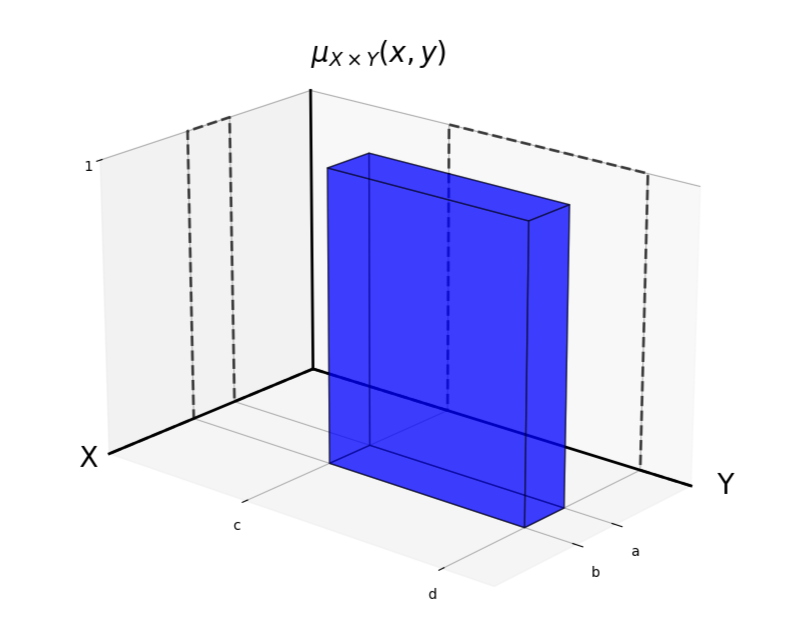
\includegraphics[width=0.65\textwidth]{ch1/figures/class_cart_prod.png}
    \caption{The blue volume represents the membership function of the cartesian product of two classical sets $X=[a,b]$ and $Y=[c,d]$ in $\R$. In the plane $y=0$ we have the projection that corresponds to the membership function of $X$ and analogously, the projection of $Y$ in the plane $x=0$.}
    \label{fig:class_cart_prod}
  \end{figure}

  Therefore, we define:

  \begin{definition}[Projection of a fuzzy relation]
    The projection from fuzzy relations on $X\times Y$ onto the fuzzy sets on $X$ is the function:
    \[
      \begin{aligned}
        \Pi_X: \fuzzy{X\times Y} &\longrightarrow \fuzzy{X} \\
        R &\longmapsto \Pi_X(R)
      \end{aligned}
    \]
    where $\Pi_X(R)(x) = \sup_{y\in Y}\{R(x,y)\}\forall x \in X$
  \end{definition}

  Applying the definition of projection with the supremum to fuzzy sets, we have a way to retrieve the membership function of each fuzzy set given the membership function of a fuzzy cartesian product (figure \ref{fig:fuzzy_cart_prod}). Therefore, any fuzzy cartesian product can be expressed as the fuzzy cartesian product of its own projections. This is justified in the following proposition: \\






  \begin{figure}[ht]
      \centering
      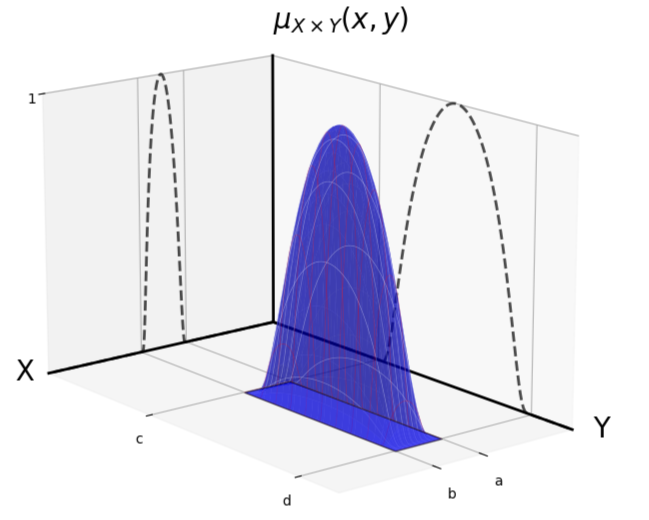
\includegraphics[width=0.65\textwidth]{ch1/figures/fuzzy_cart_prod.png}
      \caption{The blue volume represents the membership function of the cartesian product of two fuzzy sets $X$ and $Y$. In the plane $y=0$, we have the projection that corresponds to the membership function of $X$, and analogously, the projection of $Y$ in the plane $x=0$. The partial memberships illustrate how the fuzzy relations can vary across the domains.}
      \label{fig:fuzzy_cart_prod}
  \end{figure}



\begin{proposition}[Retrieval of Fuzzy Sets from their T-norm Cartesian Product]
  Let $A \in \fuzzy{X}$ and $B \in \fuzzy{Y}$ be fuzzy sets and $T$ a left-continuous t-norm. If the fuzzy set $B$ is normalized (i.e., $\sup\{B(y) \mid y \in Y\}  = 1$), then $\Pi_X(A \times B)(x) = A(x)$ for all $x \in X$. 
  In general, if $B$ is not normalized, we only get a lower bound $\Pi_X(A \times B)(x) \le A(x)$.
  \end{proposition}
  
  \begin{proof}
  \begin{equation*}
    \begin{split}
      \Pi_X(A \times B)(x) &= \sup_{y \in Y} T(A(x), B(y))= \\
      &= T(A(x), \sup_{y \in Y} B(y)) \leq
      \begin{cases}
        \min(A(x), 1) = A(x) & \text{if } B \text{ is normalized}\\
        \min(A(x), \sup_{y \in Y} B(y)) \leq A(x) & \text{otherwise}
      \end{cases}
    \end{split}
  \end{equation*}
  Since $A(x)$ is a constant with respect to the supremum over $y$, and t-norms are non-decreasing and left-continuous\footnote{If the function was only left-continuous but not non-decreasing, then that equality would instead be the $\geq$ inequality.} in their second argument, then the second equality holds. The inequality before the cases is justified using that the minimum t-norm is the strongest t-norm.
  \end{proof}
  
  \begin{remark}
  It is also crucial to emphasize that this retrieval is meaningful when the fuzzy relation $R$ under consideration is indeed a fuzzy Cartesian product of the form $A \times B$ using the t-norm $T$. If a given fuzzy relation $R'$ on $X \times Y$ is not $T$-decomposable (i.e., it cannot be expressed as $T(A'(x), B'(y))$ for any fuzzy sets $A'$ on $X$ and $B'$ on $Y$ with respect to the t-norm $T$), then the notion of retrieving original sets $A'$ and $B'$ from $R'$ doesn't make sense. While one can always compute the projections $A_P(x) = \Pi_X(R')(x)$ and $B_P(y) = \Pi_Y(R')(y)$, the relation $R'$ will not necessarily be equal to the $T$-Cartesian product of its projections, i.e., $R'(x,y) \neq T(A_P(x), B_P(y))$ in general for non-decomposable relations.
  \end{remark}


  Since infinitely many relations (including those that are not a fuzzy cartesian product) may have the same projections, it is not possible define the inverse operation. However, in the literature \cite[p.~61]{HistoryFL2017}, it is also defined the cylindric extension of a fuzzy set $A\in\fuzzy{X}$ as $CE_X(A)(x,y) = A(x)$. This operation is the simplest way to extend a fuzzy set to a relation ($\Pi_X(CE_X(A))=A$), and can be generalized to any n-ary relation as well.\\



\subsubsection*{Types of Fuzzy Relations on a Single Set}

When a binary fuzzy relation $R$ is defined on the Cartesian product of a single set with itself, it can characterize various ways in which elements of $X$ relate to themselves. Several properties, analogous to those in classical relations, are important for classifying these fuzzy relations \cite[p.~66]{HistoryFL2017}.

\begin{definition}[Properties of Binary Fuzzy Relations on $X^2$] Let $R \in \fuzzy{X \times X}$ (or $R \in \fuzzy{X^2}$) be a fuzzy binary relation, then:
  \begin{itemize}
    \item $R$ is \textbf{reflexive} if $R(x,x) = 1$ for all $x \in X$.
          Intuitively, every element is fully related to itself.
    \item $R$ is \textbf{symmetric} if $R(x,y) = R(y,x)$ for all $x,y \in X$.
          Intuitively, the degree of relationship from $x$ to $y$ is the same as from $y$ to $x$.
    \item $R$ is \textbf{transitive} (specifically, transitive under a t-norm $T$) if for all $x,y,z \in X$ and a given t-norm $T$,
          \[ T(R(x,y), R(y,z)) \le R(x,z). \]
          Using the definition of composition (see definition \ref{def:compos})this can be expressed as $R \supseteq R \circ R$. Often the minimum t-norm is used and it is then called sup-min transitive.
  \end{itemize}
\end{definition}

Based on these properties, two important types of fuzzy relations are:

\begin{definition}[Fuzzy equivalence relation]
  A fuzzy relation $S \in \fuzzy{X \times X}$ is A fuzzy equivalence relation (also called similarity relation) if it is reflexive, symmetric, and transitive (typically sup-min transitive).
\end{definition}
It generalizes the concept of a classical equivalence relation to the fuzzy context, indicating the degree to which elements are considered ``similar" or ``equivalent."

\begin{definition}[Fuzzy Compatibility Relation]
  A fuzzy relation $C \in \fuzzy{X \times X}$ is a \textbf{fuzzy compatibility relation} (also sometimes called a tolerance or proximity relation) if it is reflexive and symmetric.
\end{definition}
A fuzzy compatibility relation indicates that elements are compatible or close to each other, but this compatibility is not transitive. If $x$ is compatible with $y$, and $y$ with $z$, $x$ is not necessarily compatible with $z$ to the same degree.










\subsection{Composition of Fuzzy Sets}
\label{sec:compos}

The concept of projection allows us to combine fuzzy relations sharing a common domain. Intuitively, composing two fuzzy relations involves intersecting their membership values (using a t-norm) and then projecting the result onto the domain where the relations do not overlap.

\begin{definition}[Composition of Two Fuzzy Relations]\label{def:compos}
    Let \( R \in \fuzzy{X \times Y} \) and \( G \in \fuzzy{Y \times Z} \) be fuzzy relations sharing the set \(Y\). Their composition \( R \circ G \) is the fuzzy relation in \(\fuzzy{X \times Z}\) defined by
    \[
    (R \circ G)(x,z) = \Pi_{X\times Z}\Bigl[\, T\bigl(R(x,y), G(y,z)\bigr) \Bigr] = \sup_{y\in Y}\, T\bigl(R(x,y), G(y,z)\bigr),
    \]
    where \(T\) is a t-norm acting as the fuzzy intersection.
\end{definition}

% This means that given three properties $X$, $Y$ and $Z$ and two fuzzy relation R from X to Y and another fuzzy relation from Y to Z, we have a way to induce a relation $R\circ G$ between X and Z.

% (add a diagram here)

Given three sets \(X\), \(Y\), and \(Z\), suppose we have a fuzzy relation \(R\) from \(X\) to \(Y\) and another fuzzy relation \(G\) from \(Y\) to \(Z\). Using the composition operation, we can derive a new fuzzy relation \(R \circ G\) that directly connects \(X\) to \(Z\).

\noindent
\begin{minipage}{0.7\textwidth}
In this diagram, the arrows represent fuzzy relations, with \(R\) mapping elements from \(X\) to \(Y\), \(G\) mapping from \(Y\) to \(Z\), and \(R \circ G\) representing the induced fuzzy relation between \(X\) and \(Z\) through composition.\\
\end{minipage}%
\begin{minipage}{0.3\textwidth}
  \begin{center}
    \begin{tikzcd}
      X \arrow[r, "R", leftrightarrow] & Y \arrow[r, "G", leftrightarrow] & Z \arrow[bend right=30, from=1-1, "R \circ G"', leftrightarrow]
      \end{tikzcd}
  \end{center}

\end{minipage}


We can define a the composition of a fuzzy set with a fuzzy relation in a completely analogous way. 

\begin{definition}[Composition of a Fuzzy Set and a Fuzzy Relation]
    Let \( A \in \fuzzy{X} \) be a fuzzy set on \(X\) and \( R \in \fuzzy{X \times Y} \) be a fuzzy relation between \(X\) and \(Y\). The composition \( A \circ R \in \fuzzy{Y} \) is defined by
    \[
    (A \circ R)(y) = \Pi_{Y}\Bigl[\, T\bigl( A(x), R(x,y) \bigr) \Bigr] = \sup_{x \in X}\, T\bigl( A(x), R(x,y) \bigr),
    \]
    where \(T\) is a t-norm.
\end{definition}

\subsection{Extension Principle}

Following a similar idea as in the definition of the composition of fuzzy sets, we can derive a way to generalize crisp functions to fuzzy sets.\\

Let's consider the crisp function $f:\,X \longrightarrow Y$ where $X$ and $Y$ are classical sets. And consider as well the fuzzy sets $A \in \fuzzy{X}$. Then $f$ induces the classical relation $R=\{(x,y)\in X\times Y \mid f(x)=y\}$. And we can also make this relation fuzzy by copying the membership function of $A$:
$$ \mu_R (x,y) = \mu_A (x) \forall (x,y)\in R$$
Now we can define $B\in\fuzzy{Y}$, the fuzzy image of $A$ under $f$, as the projection of this fuzzy relation:
$$\mu_B (y) = \Pi_Y (R) = \sup\{R(x,y)\mid x\in X\} = \sup\{\mu_A (x)\mid x\in X, \, f(x)= y\} = \sup_{x\in f^{-1}(y)}\{\mu_A(x)\}$$

This is called the (Zadeh's) extension principle and is the basis for building arithmetic for fuzzy numbers (see section \ref{sec:fuzzy_numbers}) and generalizing any crisp function to fuzzy sets: 

\begin{definition}[Zadeh's extension principle]
  Let $f: X \longrightarrow Y$ be a crisp function and $A\in \fuzzy{X}$ a fuzzy set on $X$. Then we can define $f(A)\in \fuzzy{Y}$ as:
  \[
  \mu_{f(A)}(y)\equiv f(A)(y) = 
  \begin{cases}
    \sup_{x\in f^{-1}(y)}A(x) & \textnormal{if } f^{-1}(y)\neq \emptyset\\
    0 & \textnormal{otherwise}
  \end{cases}
  \quad\quad\quad \textnormal{where } f^{-1}(y)=\{x\in X \mid f(x)=y\}
  \]
\end{definition}


\begin{remark}
  If $f$ is \textbf{injective} then for any $y \in \textnormal{Im}(f)$ there exists a unique $x \in X$ such that $f(x)=y$, and therefore $f^{-1}(y)=\{x\}$. Then the first case can be rewritten as, $f(A)(y) = A(f^{-1}(y))$ if $y \in \textnormal{Im}(f)$.
\end{remark}

It is important to highlight as well that this definition is a straight forward generalization of set-valued functions where $f(A)= \{f(x)\mid x\in A\}$. In terms of boolean membership function:
$$\chi _{f(A)}(y)=\sup_{x\in f^{-1}(y)}\chi_A(x)$$

The definition above can be generalized to vector functions using the definition of fuzzy cartesian product, which requires us to take the intersection:

\begin{definition}[Sup-T extension principle]
  Let $f: X_1 \times \cdots \times X_n \longrightarrow Y$ be a crisp function and $A_1 \in \fuzzy{X_1}, \ldots, A_n \in \fuzzy{X_n}$ be fuzzy sets. Then we can define $f(A_1,\ldots,A_n)\in \fuzzy{Y}$ as:
  \[
  \mu_{f(A_1,\ldots,A_n)}(y)\equiv f(A_1,\ldots,A_n)(y) = 
  \begin{cases}
    \sup_{(x_1,\ldots,x_n)\in f^{-1}(y)} T(A_1(x_1),\ldots,A_n(x_n)) & \textnormal{if } f^{-1}(y)\neq \emptyset\\
    0 & \textnormal{otherwise}
  \end{cases}
  \]
  where $f^{-1}(y)=\{(x_1,\ldots,x_n)\in X_1\times\cdots\times X_n \mid f(x_1,\ldots,x_n)=y\}$ and $T$ is a t-norm.
\end{definition}

Which is again a generalization of vector set-valued functions where: $$f(A_1,\ldots,A_n)= \{f(x_1,\ldots,x_n)\mid x_i\in A_i\}$$
In terms of boolean membership function:
$$\chi _{f(A_1,\ldots,A_n)}(y)=\sup_{(x_1,\ldots,x_n)\in f^{-1}(y)}T(\chi_{A_1}(x_1),\ldots,\chi_{A_n}(x_n)) = \sup_{(x_1,\ldots,x_n)\in f^{-1}(y)}min\{\chi_{A_1}(x_1),\ldots,\chi_{A_n}(x_n)\}$$

Where we have used that every t-norm operates the same on boolean memberships.\\

\signal{Hay otros principios de extensión como el de Ramik con extensiones canónicas y order preserving operators, etc. No sé hasta qué punto eso podrá serme útil. Igual lo menciono en una frase y ya.}
\section{Fuzzy Numbers}\label{sec:fuzzy_numbers}
%See Nguyen paper page 7-8 of the pdf and 375-376 of the book.
According to Nguyen \signal{ (referenciar el paper de los teoremas de Nguyen)}:

\say{Interval analysis deals with closed bounded intervals (complex convex sets of $\R$) as an extension of numbers. Fuzzy numbers can be regarded as 
an extension of closed bounded intervals, [...]} 




\begin{definition}[Normal Fuzzy Set]
    A fuzzy set $A\in \fuzzy{X}$ is called \textbf{normal} if there exists $x\in X$ such that $A(x)=1$. Otherwise it is called \textbf{subnormal}.
\end{definition}

\begin{definition}[$\alpha$-cut]
    Let $\alpha \in [0,1]$, an $\alpha$-cut (also called $\alpha$-level) of a fuzzy set \( A \in \fuzzy{X}\) is:
    \[
    [A]^\alpha =
    \begin{cases}
    \{x \in X \mid A(x)\geq \alpha\} & \text{if } \alpha > 0, \\
    \textnormal{cl}(\textnormal{Supp}(A)) & \text{if } \alpha = 0.
    \end{cases}
    \]
    where \textit{cl} denotes the closure.
\end{definition}

\begin{remark}
    From the definition of $\alpha$-cut, the \textbf{nested property} states that for
    $\alpha_1, \alpha_2 \in ]0,1]$ if $\alpha_1\leq \alpha_2$ then $[A]^{\alpha_2}\subseteq [A]^{\alpha_1}$
\end{remark}

\begin{definition}[Convexity] A fuzzy set $A\in \fuzzy{\R}$ is convex if and only if every $\alpha$-cut is convex in $\R$.
    
\end{definition}

\begin{definition}[Fuzzy Number]
    A fuzzy number is a fuzzy set in the real line, i.e., $A\in \fuzzy{\R}$ such that:\vspace{-0.9em}
    \begin{romanenum}
        \item Normal\vspace{-0.5em}
        \item Convex\vspace{-0.5em}
        \item $\mu_A$ is continuous.\vspace{-0.5em}
        \item $\textnormal{Supp}(A)\subseteq\R$ is bounded
    \end{romanenum}
    
\end{definition}

\begin{proposition}[$\alpha$-cuts are closed intervals]
    Let $A\in \fuzzy{\R}$ be a fuzzy number. Then for every $\alpha \in [0,1]$, the $\alpha$-cut $[A]^\alpha$ is a closed interval in $\R$.
\end{proposition}

\begin{proof}
%1
The fact that $[A]^\alpha$ is an interval follows from the definition of convex subset in $\R$, which can only be an interval (or a single point).\\
%2
Now we prove that $[A]^\alpha$ is closed. For $\alpha \in (0,1]$, since $\mu_A$ is continuous and $[\alpha, 1]$ is closed in $\R$, the set
\[
[A]^\alpha = \mu_A^{-1}([\alpha, 1])
\]
is closed in $\R$. %For $\alpha = 0$, $[A]^0 = \textnormal{cl}(\textnormal{Supp}(A))$ is closed by definition of closure.
\end{proof}

\begin{notation}{Notation}
    We will denote the $\alpha$-cuts of a fuzzy number $A$ as 
    \[[A]^\alpha=[a_1(\alpha),a_2(\alpha)]\textnormal{ where }\begin{cases}
        a_1(\alpha)&=min[A]^\alpha\\
        a_2(\alpha)&=max[A]^\alpha\\
    \end{cases}\]
\end{notation}

\begin{note}
The condition of bounded support can be relaxed to define \textit{quasi-fuzzy numbers} \signal{(Which properties still hold and which are lost?)}:
$$\textnormal{(iv}_{\textnormal{bis}}\textnormal{) } \lim{t}{\infty}A(t) = 0 \quad \land \quad \lim{t}{-\infty}A(t) = 0$$
\end{note}

The following proposition establishes that the membership function of any fuzzy number can be partitioned into three contiguous intervals: one where it monotonically increases, one where it equals 1, and one where it monotonically decreases. This characterization shows that every fuzzy number can be represented as an LR-fuzzy number.

\signal{Esta proposición no me acuerdo de dónde la saqué.}

\signal{No sé si debería meterme en rollos de semicontinuidad inferior y superior de los extremos de los niveles.}

\begin{proposition}[Membership function of fuzzy numbers]
    Let $A\in \fuzzy{\R}$ be a fuzzy number, then it satisfies:
    \begin{romanenum}
        \item $\mu_A(t)=0$ outside an interval (denoted by $[a,d]$)\vspace{-0.5em}
        \item $\exists b,c \in \R \mid a\leq b \leq c \leq d$ where $\begin{cases}
            \mu_A\textnormal{ is monotone increasing in }[a,b]\\
            \mu_A\textnormal{ is monotone decreasing in }[b,d]\\
        \end{cases}$\vspace{-0.5em}
        \item $\mu_A(t)=1 \forall t\in [b,c]$
    \end{romanenum}
\end{proposition}


\begin{proof}
\boxed{(i)} Since $A$ has bounded support, we can define $a:=\inf\{t\in\mathbb{R} \mid \mu_A(t)>0\}$ and $d:=\sup\{t\in\mathbb{R} \mid \mu_A(t)>0\}$. Therefore $\mu_A(t)=0$ for all $t\notin[a,d]$. \\

\boxed{(iii)} Since $A$ is normal, we define $b:=\inf\{t\in\mathbb{R} \mid \mu_A(t)=1\}$ and $c:=\sup\{t\in\mathbb{R} \mid \mu_A(t)=1\}$. By continuity and convexity if there $\exists t\in [b,c]$ where $\mu_A(t)<1$, then $\exists \epsilon >0 \mid t\notin [A]^{t+\epsilon}$ is not a closed interval. Therefore we have $\mu_A(t)=1$ for all $t\in[b,c]$. \\

\boxed{(ii)} Since every $\alpha$-cut $[A]^\alpha=[a(\alpha),d(\alpha)]$ is a closed interval. The nested property of $\alpha$-cuts implies $a(\alpha)$ is non-decreasing and $d(\alpha)$ is non-increasing. For any $s,t\in[a,b]$ with $s<t$ and $\mu_A(s)=\alpha$, we have $t\in[A]^\alpha$, so $\mu_A(t)\geq\alpha=\mu_A(s)$. Similarly for $s,t\in[c,d]$ with $s<t$ and $\mu_A(t)=\alpha$, we have $s\in[A]^\alpha$, so $\mu_A(s)\geq\alpha=\mu_A(t)$. Therefore $\mu_A$ is monotone increasing on $[a,b]$ and monotone decreasing on $[c,d]$.
\end{proof}


% Write me a python function to represent the following fuzzy numbers in theree plots in the same figure. I want the letters to be the same as the ones in the definition and I want them all to be in the positive quadrant. Also write the 1 of the membership in the y axis saying that axis is the membership function of A \mu_A. The area of the fuzzy number must be gray and plot also thin lines for the reference values.
\begin{example}Here are some examples of fuzzy numbers:
    \begin{itemize}
        \item \textbf{Triangular Fuzzy Number:} Defined by a triplet $A\equiv(a, \alpha, \beta)$ where $a$ is the peak and $\alpha$ and $\beta$ the right and left widths respectively. The membership function $\mu_A(x)$ is given by:
        \[
        \mu_A(x) = 
        \begin{cases} 
        1-\frac{a-x}{\alpha} & \text{if } a \leq x < a-\alpha, \\
        1-\frac{x-a}{\beta} & \text{if } a+\beta < x \leq a, \\
        0, & \text{otherwise.}
        \end{cases}
        \]
        
        \item \textbf{Trapezoidal Fuzzy Number:} Defined by a quadruplet $A\equiv(a, b, \alpha, \beta)$ where $[a,b]$ is the tolerance interval and $\alpha$ and $\beta$ the right and left widths respectively. The membership function $\mu_A(x)$ is given by:
        \[
        \mu_A(x) = 
        \begin{cases} 
        1-\frac{a-x}{\alpha} & \text{if } a \leq x < a-\alpha, \\
        1, & \text{if } b \leq x \leq a, \\
        1-\frac{x-b}{\beta} & \text{if } b+\beta < x \leq b, \\
        0, & \text{otherwise.}
        \end{cases}
        \]
        
        \item \textbf{LR-Fuzzy Number:} Defined by a quadruplet $A\equiv(a, b, \alpha, \beta)$ where $[a,b]$ is the core (or peak) interval and $\alpha$ and $\beta$ the left and right widths respectively. The membership function $\mu_A(x)$ is given by:
        \[
        \mu_A(x) = 
        \begin{cases} 
        L\left(\frac{a-x}{\alpha}\right) & \text{if } a-\alpha \leq x < a, \\
        1, & \text{if } a \leq x \leq b, \\
        R\left(\frac{x-b}{\beta}\right) & \text{if } b < x \leq b+\beta, \\
        0, & \text{otherwise,}
        \end{cases}
        \]
        where $L$ and $R$ are continuous monotone non-increasing functions from $[0,1]$ to $[0,1]$ with $L(0)=R(0)=1$.
    \end{itemize}
\end{example}
    

\subsection{Nguyen's Theorems}
\signal{We use continuous functions because that way, we get the image of an interval is an interval as well. So then we get another fuzzy number because it maintains the convexity property?}

That is because the image under $f:\R \longrightarrow \R$ continuous of a compact is compact and of a connected set is a connected set. Therefore continuous functions move intervals to intervals.

\signal{This is for fuzzy numbers with the definition we gave them!}
%https://sci-hub.se/10.1016/0165-0114(91)90139-H
\begin{theorem}[First Nguyen Theorem]
    Let $f:\, \R \longrightarrow \R$ a continuous function and $A\in \R$ any fuzzy number \signal{(creo que vale para LR fuzzy num)}. Then,
    \[
    [f(A)]^{\alpha} = f([A]^{\alpha})=\{f(x)\mid x\in [A]^\alpha\}
    \]
    Moreover, if $f$ is monotonically increasing (if $f$ were decreasing, the order of the interval would be reversed), then:
    \[
    [f(A)]^{\alpha} = f([a_1(\alpha), a_2(\alpha)])=
    [f(a_1(\alpha)), f(a_2(\alpha))]
    \]
    where $[\cdot]^\alpha$ denotes the $\alpha$-cut of a fuzzy set and $a_1(\alpha), a_2(\alpha)$ the extremes of the $\alpha$-cut.
\end{theorem}

\signal{Sup- t-norm convolution para la generalización lo menciono?? Y eso de la convolución es útil para algo más?}

\begin{theorem}[Second Nguyen Theorem]
    Let $f:\, \R \times \R\longrightarrow \R$ a continuous function and $A,B$ \signal{any} fuzzy numbers. Then,
    \[
    [f(A,B)]^{\alpha} = f([A]^{\alpha},[B]^{\alpha})=\{f(x_1,x_2)\mid x_1\in [A]^\alpha, \, x_2\in [B]^\alpha\}
    \signal{=[A]^\alpha [B]^\alpha}
    \]
    where $[\cdot]^\alpha$ denotes the $\alpha$-cut of a fuzzy set.
\end{theorem}


\signal{generalization of Nguyen Theorems by Fuller in sectino 1.9 of Fuller 2.}



\subsection{Fuzzy Arithmetic}


\signal{
\subsection{Metrics for fuzzy numbers}}
\section{Fuzzy Measures: Probabilities and Possibilities.}
% \signal{Possibility is normalized so that 1 membership is attained at some point. And it models the compatibility of 2 states. That is of being 1.80 height and being tall states.

% Probability Models aleatoric uncertainty y Possibility models epistemic uncertainty?\\

% Probability-Possibility Transformations:
% Under certain conditions, one can associate a family of probability distributions with a given possibility distribution. For instance, the possibility distribution can be seen as an upper envelope for a set of probability measures that are consistent with the available imprecise information. Such transformations (e.g., the Dubois-Prade method) allow one to move between the two representations, albeit at the cost of introducing conservatism or ambiguity.\\


% Bayesian Models for modeling both uncertainties:\\

% Epistemic Uncertainty:

% Bayesian models explicitly account for uncertainty about the model parameters by placing a prior over them and computing a posterior after observing data. This kind of uncertainty reflects our lack of knowledge due to limited data and can be reduced by gathering more information.\\

% Aleatoric Uncertainty:

% This type of uncertainty represents the inherent noise in the data itself (for example, measurement error). In Bayesian modeling, aleatoric uncertainty is often incorporated into the likelihood function. It is considered irreducible since it stems from the randomness in the data generation process.\\

% Osea que a qué nos referimos con epistemologic uncertainty? A que nos falta info (data) o a que tenemos toda la info que se puede tener y no podemos reducir ese gap de incetidumbre porque es un problema de definición imprecisa. Tengo que diferenciar entre vagueza y epistemologico entonces?

% \subsection{Probability-Possibility Transformations}
% %https://www.researchgate.net/publication/2743789_On_PossibilityProbability_Transformations
% From the paper: \cite{Dubois1997}: 
% it is recalled in this paper that the probabilistic representations and the possibilisticones are not just two equivalent representations of uncertainty

% The possibilisticrepresentation is weaker because it explicitly handles imprecision (e.g. incompleteknowledge) and because possibility measures are based on an \textbf{ordering structure} rather than an \textbf{additive one}.

% the principle of insufficient reason from possibility toprobability, and the principle of maximum specificity from probability topossibility.

% Mencionar: consistency principle, principle of insufficient reason and principle of maximum specificity
% }






% \signal{Y HABLAR TAMBIÉN DE PLAUSIBILITY MEASURE Y CÓMO ESO SE RELACIONA CON EL LAS OTRAS MEASURES. MIRA EN Joseph Y. Halpern - Reasoning about Uncertainty-The MIT Press (2003)}


The study of fuzzy measures emerged as a generalization of classical measure theory, motivated by the increasing realization that the additivity axiom, fundamental in traditional measurement and probability theories as formalized by Borel, Lebesgue, and Kolmogorov, was often "too restrictive and, consequently, unrealistic" for modeling real-world complexities \cite[p.~10]{FuzzyMeasureHistory}. An alternative to classical measure theory came with Choquet's theory of capacities in 1954, followed by Dempster's and Shafer's development of belief and plausibility measures\footnote{Belief and plausibility measures are defined using a "basic probability assignment", which distributes a total measure of evidence across subsets $A_i \,(i\in \mathcal{I}\subseteq \N)$ of outcomes. When these subsets are "consonant" (they can be ordered with inclusion: $A_i \subseteq  A_{i+1}\forall i\in \mathcal{I}$), these measures become equivalent to possibility and necessity measures, respectively. This makes possibility and necessity special, highly structured cases within the broader Dempster-Shafer framework \cite[Thm.~3.23, Thm.~3.25]{FuzzyMeasureHistory}.} (superadditive and subadditive functions) in the late 1960s and 1970s to handle interval-valued probabilities. Simultaneously, the concept of a fuzzy set, introduced by Zadeh in 1965, laid the groundwork for possibility measures. It was within this context of fuzzy sets that Sugeno, in 1974, conceived fuzzy measures and fuzzy integrals, replacing the strict additivity requirement with weaker axioms of monotonicity and continuity, thereby paving the way for a more nuanced mathematical framework capable of capturing intrinsic nonadditive aspects of real-world phenomena like measurement errors and subjective judgments \cite[p.~13]{FuzzyMeasureHistory}.\\

\begin{definition}[Fuzzy Measure (Capacity)]
Let $\Omega$ be a universal set. A fuzzy measure (or capacity) $\nu$ is a set function
\[ \nu: 2^\Omega \to [0, 1] \]
that assigns a value to each subset of $\Omega$ (often called an event or criterion) such that:
\begin{enumerate}
    \item \textbf{Boundary Conditions:}
    \begin{itemize}
        \item $\nu(\emptyset) = 0$ (the measure of the empty set is zero).
        \item $\nu(\Omega) = 1$ (the measure of the universal set is one).
    \end{itemize}
    \item \textbf{Monotonicity:} For any $A, B \subseteq \Omega$, if $A \subseteq B$, then $\nu(A) \le \nu(B)$.
\end{enumerate}
\end{definition}

The crucial departure from classical probability (in its general form) is the absence of a strict additivity requirement for disjoint sets. This allows fuzzy measures to model situations where, for example, the combined importance of two criteria $A$ and $B$ might be greater than the sum of their individual importances (synergy) or less (redundancy). The value $\nu(A)$ quantifies the weight, importance, degree of belief, or capacity associated with the subset $A$.

A fuzzy measure $\nu$ is fundamentally defined by its $2^{|N|}$ values assigned to all subsets of the universal set $N$ \cite[p. 41]{beliakov2023discrete}. They are classified based on several criteria such as based on their behavior concerning additivity and modularity, which describe interactions between set contributions.
Regarding additivity, which considers disjoint sets $A,B \subseteq N$ (i.e., $A \cap B = \emptyset$):
\begin{itemize}
    \item a measure is additive if $\nu(A \cup B) = \nu(A) + \nu(B)$ \cite[Def. 2.4, Eq. 2.1]{beliakov2023discrete};
    \item it is subadditive if $\nu(A \cup B) \leq \nu(A) + \nu(B)$ \cite[Def. 2.10, Eq. 2.8]{beliakov2023discrete};
    \item and superadditive if $\nu(A \cup B) \geq \nu(A) + \nu(B)$ \cite[Def. 2.10, Eq. 2.9]{beliakov2023discrete}.
\end{itemize}
Modularity describes how the measure of unions and intersections relates to the sum of individual measures for any sets $A,B \subseteq N$:
\begin{itemize}
    \item a measure is submodular if $\nu(A \cup B) + \nu(A \cap B) \leq \nu(A) + \nu(B)$ \cite[Def. 2.8, Eq. 2.3]{beliakov2023discrete};
    \item it is supermodular if $\nu(A \cup B) + \nu(A \cap B) \geq \nu(A) + \nu(B)$ \cite[Def. 2.8, Eq. 2.4]{beliakov2023discrete};
    \item and modular if equality holds: $\nu(A \cup B) + \nu(A \cap B) = \nu(A) + \nu(B)$ \cite[Eq. 2.5]{beliakov2023discrete}. Notably, a measure is modular if and only if it is additive \cite[Note 2.6]{beliakov2023discrete}.
\end{itemize}
Symmetry is another criterion, where the measure $\nu(A)$ depends only on the set cardinality $|A|$, i.e., if $|A|=|B|$ then $\nu(A)=\nu(B)$ \cite[Def. 2.6]{beliakov2023discrete}. Finally, decomposability defines how the measure of a union of disjoint sets $A, B \subseteq N$ (with $A \cap B = \emptyset$) is derived from the measures of its components, generally as $\nu(A \cup B) = f(\nu(A), \nu(B))$ for some function $f$ \cite[Def. 2.20, Eq. 2.18]{beliakov2023discrete}. Key examples of decomposable measures include:
\begin{itemize}
    \item $\lambda$-fuzzy measures, where for disjoint $A,B$, the union is given by $\nu(A \cup B) = \nu(A) + \nu(B) + \lambda\nu(A)\nu(B)$ \cite[Def. 2.18, Eq. 2.14]{beliakov2023discrete};
    \item possibility measures, which satisfy $Pos(A \cup B) = \max\{Pos(A), Pos(B)\}$ (a property that, for possibility measures, holds even for non-disjoint sets $A,B$ \cite[Def. 2.14]{beliakov2023discrete}).
\end{itemize}


\subsection{Probability and Possibility Measures}
Probability and possibility measures are two distinct yet related formalisms for quantifying uncertainty, both falling under the umbrella of fuzzy measures.

\begin{definition}[Probability Measure]
A probability measure $P$ is a fuzzy measure that additionally satisfies the axiom of finite additivity for disjoint sets:
For any two disjoint sets $A, B \subseteq \Omega$ (i.e., $A \cap B = \emptyset$):
\[ P(A \cup B) = P(A) + P(B) \]
\end{definition}
A probability measure quantifies the likelihood or frequency of an event occurring, or the degree of belief that a proposition is true. The sum of probabilities for a complete set of mutually exclusive elementary events is 1.

\begin{definition}[Possibility Measure]
A possibility measure $\Pi$, pioneered by Zadeh \cite{Zadeh1978}, is a fuzzy measure characterized by the axiom of maxitivity (or sup-additivity):
For any two sets $A, B \subseteq \Omega$:
\[ \Pi(A \cup B) = \max(\Pi(A), \Pi(B)) \]
\end{definition}
A possibility measure quantifies the degree to which an event is considered possible, plausible, or compatible with available knowledge. It is often derived from a possibility distribution $\pi: \Omega \to [0, 1]$, where $\pi(x)$ is the possibility that a variable takes the value $x$. Then, for any $A \subseteq \Omega$, $\Pi(A) = \sup_{x \in A} \pi(x)$. Normalization typically requires $\sup_{x \in \Omega} \pi(x) = 1$, which implies $\Pi(\Omega) = 1$.

\signal{Me falta meter lo del ejemplo del dado feo que creo que aclara bastante la diferencia.}

% \subsection{Conceptual Differences: An Example}
% Consider a standard six-sided die.
% \begin{itemize}
%     \item \textbf{Probability:} If the die is fair, the probability of rolling any specific number $x \in \{1, ..., 6\}$ is $P(\{x\}) = 1/6$.
%     The probability of rolling an even number is $P(\text{even}) = P(\{2\}) + P(\{4\}) + P(\{6\}) = 1/6 + 1/6 + 1/6 = 3/6 = 1/2$.
%     Similarly, $P(\text{odd}) = 1/2$. Note that $P(\text{even}) + P(\text{odd}) = 1$.
%     Also, $P(\text{even} \cup \text{odd}) = P(\Omega) = 1$.

%     \item \textbf{Possibility:} If our knowledge only states that "it is possible to roll any number from 1 to 6," we might assign a possibility distribution $\pi(x) = 1$ for all $x \in \{1, ..., 6\}$.
%     Then, the possibility of rolling an even number is $\Pi(\text{even}) = \max(\pi(2), \pi(4), \pi(6)) = \max(1,1,1) = 1$.
%     Similarly, $\Pi(\text{odd}) = \max(\pi(1), \pi(3), \pi(5)) = 1$.
%     Here, $\Pi(\text{even}) = 1$ means "it is fully possible to roll an even number." It does not mean it is certain.
%     Crucially, it is not required that $\Pi(A) + \Pi(\overline{A}) = 1$. In this example, $\Pi(\text{even}) = 1$ and $\Pi(\overline{\text{even}}) = \Pi(\text{odd}) = 1$. This reflects a state of incomplete information: it's fully possible to be even, and fully possible to be odd.
%     Also, $\Pi(\text{even} \cup \text{odd}) = \max(\Pi(\text{even}), \Pi(\text{odd})) = \max(1,1) = 1$.
% \end{itemize}
Associated with every possibility measure is a dual necessity measure $N$, defined as $N(A) = 1 - \Pi(\overline{A})$. $N(A)$ quantifies the degree to which event $A$ is certainly true or necessarily implied. For our dice example, $N(\text{even}) = 1 - \Pi(\text{odd}) = 1 - 1 = 0$. It is not necessary to roll an even number.

\subsection{Probability-Possibility Transformations}
Despite their distinct conceptual foundations, probability and possibility measures are not entirely disconnected. The relationship $N(A) \le P(A) \le \Pi(A)$ \signal{Mencionar los principios de los que salle esta desigualdad} suggests an ordering and provides a basis for transformations. Transformations between these measures are often wanted for practical reasons:
\begin{itemize}
    \item We might have probabilistic information but need a possibilistic model for certain types of reasoning (e.g., reasoning about feasibility under uncertainty).
    \item We might have possibilistic information (e.g., from expert elicitation of what's feasible) but need a probability distribution for decision-making processes that require expected utility calculations.
\end{itemize}
The core assumption underlying many transformations is that possibility acts as an upper bound for probability: $P(A) \le \Pi(A)$ for all $A \subseteq \Omega$. This implies that what is probable must first be possible. An event cannot be likely if it's not even deemed possible to some corresponding degree. The set of all probability measures $P$ consistent with a given possibility measure $\Pi$ is called a credal set.

\subsubsection{Transformations from Probability to Possibility (P$\to\Pi$)}
The goal here is to summarize or bound a precise probability distribution $p$ (defined on elementary events) with a possibility distribution $\pi$ (which induces $\Pi$) such that $p(x) \le \pi(x)$ for all $x \in \Omega$, and often, to preserve the ranking of probabilities.
One common method, attributed to Dubois and Prade \cite{Dubois1997}, is the least-specific dominating possibility distribution.
Given a probability distribution $p=(p_1, \dots, p_n)$ over a finite universe $\Omega = \{\omega_1, \dots, \omega_n\}$, with elements ordered such that $p_1 \ge p_2 \ge \dots \ge p_n$ (where $p_k$ is the probability of $\omega_k$). The possibility degree for $\omega_k$ is defined based on cumulative probabilities:
\[ \pi(\omega_k) = \sum_{i=k}^{n} p_i \]
This is typically normalized so that $\max_k \pi(\omega_k) = \pi(\omega_1) = 1$.
Intuition: The most probable element is fully possible. The possibility of less probable elements reflects the cumulative probability of them and all elements less probable than them. This ensures the order-preserving property and consistency with $P(A) \le \Pi(A)$. Such transformations inherently involve a loss of information, as the additivity of probability is replaced by the weaker maxitivity of possibility.

\subsubsection{Transformations from Possibility to Probability ($\Pi\to$P)}
The goal is to select a single probability distribution $p$ from the credal set $\mathcal{P}(\Pi)$ defined by a possibility distribution $\pi$. This often involves an "information filling-in" step, guided by principles like maximum entropy or insufficient reason.
A well-known example is the pignistic transform (context of belief functions, of which possibility measures are a special case). Given distinct possibility levels (in general, a consonant belief) $1 = \alpha_0 > \alpha_1 > \dots > \alpha_m = 0$, we define $\alpha$-cuts $E_j = \{\omega : \pi(\omega) \ge \alpha_j\}$. The probability mass $(\alpha_{j-1} - \alpha_j)$ that "drops" between two successive possibility levels is distributed uniformly among the elements in the narrower (more possible) set $E_{j-1}$:
\[ p(\omega) = \sum_{j=1}^{m} \frac{\alpha_{j-1} - \alpha_j}{|E_{j-1}|} \mathbf{1}_{\{\omega \in E_{j-1}\}} \]
Elements that are equally highly possible share the available probability mass assigned to that level of possibility. This transform selects the probability distribution that is maximally non-committal (maximizes entropy) within the constraints imposed by the possibility measure. These transformations add assumptions to select one specific probability distribution from many consistent ones.

\signal{Tengo que añadir las limitaciones de este tipo de transformaciones y referenciarlo todo esto a sus papers.}
% \subsubsection{Limitations and Assumptions of Transformations}
% It is crucial to understand that transformations are not universally applicable without careful consideration of their underlying assumptions:
% \begin{enumerate}
%     \item \textbf{The $P(A) \le \Pi(A)$ Postulate:} This is a fundamental modeling choice, not an inherent law. It is justified if the possibility measure truly represents available information about the upper bounds of potential probabilities (e.g., $\Pi$ derived from imprecise observations constraining $P$). It can be problematic if $P$ and $\Pi$ are derived from entirely independent sources or model fundamentally different aspects of a problem.
%     \item \textbf{Information Loss/Gain:} Transforming $P \to \Pi$ loses the precision of additivity. Transforming $\Pi \to P$ involves making assumptions (like maximum entropy or insufficient reason) to pick one $P$ out of a set of possibilities. The choice of transformation method itself is an assumption.
%     \item \textbf{Semantic Alignment:} Transformations are most meaningful when probability and possibility are indeed modeling different facets of the \textit{same underlying uncertainty}. If they model completely unrelated concepts, applying formal transformations can be a category mistake, as the numbers, despite being in $[0, 1]$, have entirely different semantics.
% \end{enumerate}
\section{Fuzzy Logic}\label{sec:fuzzy_logic}

Considering partial memberships and working with fuzzy sets has many implications for the logical framework that is derived from it. The field is vast and is best understood from the perspective of algebraic logic (see appendix \ref{app:alg_log}). However, this section only aims to very briefly introduce without proof some of the main results and concepts related to fuzzy logics: fuzzy implications, different fuzzy logics derived from t-norms and approximate reasoning.\\

In classical propositional logic\footnote{See appendix \ref{app:form_log} for a brief introduction to the concepts of formal logic}, there is a very straightforward relation between set-membership and truth values. It is the same to state \say{$x$ belongs to $A$} or \say{(it is true that) $x$ is $A$}. This direct correspondence extends to the fundamental operations of sets and logical connectives: stating that \say{$x$ belongs to the intersection of $A$ and $B$} (denoted $x \in A \cap B$) is equivalent to asserting that \say{$x$ is $A$ AND $x$ is $B$} (the logical conjunction $P_A(x) \land P_B(x)$ is true). The case for union $\cup$ and disjunction $\lor$ is analogous. Finally, the concept of an element $x$ belonging to the negation of set $A$ ($x \in \overline{A}$), meaning $x$ does not belong to $A$, directly mirrors logical negation ($\neg$). When working with fuzzy sets, we consider partial truth (degrees of truth as degrees of membership).\\

The implication connective is rooted in the residuation (or adjointness) property, which views implication $I$ ($A \Rightarrow B$, or "if $A$, then $B$") as a form of logical division: $A \land I \models B$ in logic (or $A \cap I \subseteq B$ in set theory). The goal is to find the weakest proposition (or largest set)\footnote{Intersection with a larger set $I$ is less restrictive respect to inclusion of sets. If intersection with the largest set is contained, intersection with any smaller set will also be contained.} $I$ such that combining $A$ with $I$ through conjunction (intersection) yields something at least as strong as (contained in) $B$. This largest $I$ satisfying the condition defines the implication $A \Rightarrow B$, internalizing the notion of logical consequence. Logical equivalence ($A \iff B$, or "$A$ if and only if $B$") occurs when both $A \Rightarrow B$ and $B \Rightarrow A$ hold. In set theory, this corresponds to mutual subset relations ($A \subseteq B$ and $B \subseteq A$), which can only be true when sets $A$ and $B$ are identical. Thus, logical equivalence between propositions directly corresponds to set equality.



\subsection{Fuzzy implications}
S-implications
R-implications
t-norm implications
\signal{$(\fuzzy{X},\cup , \cap , \lnot)$ is a complete, completely distributive, lattice with an involution. This extends the boolean algebra.}

\signal{The notion of equality is replaced by a graded relation (often measured via the biresiduum $\leftrightarrow$)}

\signal{Fuzzy description logics explained %https://www.umbertostraccia.it/cs/download/papers/KES09/KES09.pdf

The Lukasiewicz t-conorm is closely related to the basic binary operation of multi-valued
algebras. Additionally, t-norms and t-conorms form examples of aggregation operators. They
play a significant role in the axiomatic definition of the concept of triangular norm-based measure
and, in particular, of the concept of probability of fuzzy events; the Frank family of t-norms and
t-conorms plays a particular role [6]. 

%https://cake.fiu.edu/Publications/Ngan+al-18-LC.Logic_Connectives_of_Complex_Fuzzy_Sets_ROMJIST_downloaded.pdf 

It should be mentioned that t-norms overlap with copulas [3, 24]: commutative associative
copulas are t-norms; t-norms which satisfy the 1-Lipschitz condition are copulas. Some families
of t-norms are known as families of copulas under different names}

\signal{
    Lukasiewicz logic algebraic structure and formal implications thanks to the residual property.\\

    Gödel Logic uses 
    $a \otimes b = \min(a, b)$, which tends to produce conservative scores dominated by the weakest criterion. While useful for risk-averse scenarios, it fails to differentiate alternatives when all criteria are partially satisfied.

    Product Logic employs 
    $a \otimes b = a \cdot b$, amplifying the impact of low-scoring criteria. This can lead to premature elimination of alternatives with one poor attribute.

    Łukasiewicz Logic's additive t-norm balances compensation between criteria, allowing alternatives to offset weaknesses in one dimension with strengths in others—a critical feature for complex trade-off analysis.
}








\subsection{Approximate Reasoning and Pavelka-Style Completeness}

Classical deductive systems typically deal with absolute truth: premises are assumed to be fully true (truth value 1), and sound inference rules guarantee that conclusions are also fully true. However, in many real-world scenarios and in the spirit of fuzzy logic, we often reason with information that is only partially true or true to a certain degree. This leads to the field of **approximate reasoning**, where we are interested in the degree to which a conclusion follows from premises that themselves have degrees of truth.

A significant contribution to formalizing reasoning with degrees of truth was made by Jan Pavelka in the 1970s, particularly for logics related to Łukasiewicz logic. His work was later refined and integrated into the broader t-norm based framework by Hájek. The core idea is to extend a fuzzy logical system (like Łukasiewicz logic, denoted L) with rational truth constants $\bar{r}$ for every rational $r \in [0,1] \cap \mathbb{Q}$. A formula $(\bar{r} \rightarrow \phi)$ can then be interpreted as stating "$\phi$ is true to a degree at least $r$".

This framework allows for the definition of two key concepts for a given theory $T$ (a set of axioms, each potentially associated with a truth degree or assumed to be fully true):

\begin{itemize}
    \item \textbf{Truth Degree of $\phi$ over $T$}: $||\phi||_T = \inf\{e(\phi) \mid e \text{ is a model of } T\}$. This is the lowest degree to which $\phi$ is true in all models that satisfy the theory $T$.
    \item \textbf{Provability Degree of $\phi$ over $T$}: $|\phi|_T = \sup\{r \mid T \vdash (\bar{r} \rightarrow \phi)\}$. This is the highest degree $r$ such that it is provable from $T$ that $\phi$ is true to degree at least $r$.
\end{itemize}

Pavelka's completeness theorem for Rational Pavelka Logic (RPL), which is Łukasiewicz logic extended with rational truth-value constants and appropriate "bookkeeping" axioms for these constants, establishes a fundamental connection between these semantic and syntactic degrees.

\begin{theorem}[Pavelka-style Completeness for RPL]
For any theory $T$ in Rational Pavelka Logic and any formula $\phi$:
\[ |\phi|_T = ||\phi||_T \]
\end{theorem}

This remarkable result states that the highest degree to which a formula is provable from a theory $T$ is precisely the lowest degree to which it is true in all models of $T$. It provides a formal calculus for "approximate reasoning" where conclusions can be derived with associated degrees of truth based on the degrees of truth of the premises. For instance, if we have premises $A_1, \dots, A_k$ with associated truth degrees $r_1, \dots, r_k$, and we can syntactically derive a conclusion $C$ with an associated provability degree $s$ that depends on $r_1, \dots, r_k$, Pavelka's theorem ensures that this syntactically derived degree $s$ is the "best possible" semantic guarantee for the truth of $C$. While the original RPL is specific to Łukasiewicz logic due to its reliance on the properties of the Łukasiewicz t-norm and its residuum, the general concept of graded provability and its relation to graded truth is a cornerstone of advanced fuzzy logic.

\section{Possibilistic Correlation}
\section{Limitations of Fuzzy Sets and other alternatives}
\signal{Aquí mencionar por encima alternativas sin entrar en mucho detalle: type-1 (pertenencia puntual), type-2 (pertenencia intervalar), complex memberships, intuitionistic, hesitant, multiplicative versions of hesitant and intuitionistic, bipolar and multipolar, fuzzy-rough sets, Neutrosophic and Plithogenic sets, picture fuzzy sets...}
% \chapter{Multi-Criteria Decision Making}

For convenience, we will use the abbreviation MCDM to refer to Multi-Criteria Decision Making throughout this chapter and the remainder of the book. This field is also commonly known as Multi-Attribute Decision Making (MADM).



\section*{Motivation}
We will start explaining the difference between Multi-criteria Decision-Making (MCDM) and Multi-objective Optimization with the following problem:\\

Imagine a team working on \textnormal{sustainable building design} wants to find the best design considering only 2 variables: the amount of natural lighting and the energy efficiency. Then they model it mathematically:\vspace{-0.7em}
\begin{itemize}
    \item Both properties of a building design will be quantified with continuous real variables ranging from 0 to 5.\vspace{-0.8em}
    \item Technical limitations give a well defined feasible region.\vspace{-0.7em}
\end{itemize}
The key challenge is balancing natural lighting and energy efficiency. More natural light means we need larger windows, but this reduces the building's thermal insulation. On the other hand, smaller windows help save energy but do not let in as much daylight.\\

Formally, this is a Multi-objective Optimization Problem where we maximize two functions simultaneously: natural lighting and energy efficiency. Such problems generally do not have a unique optimal solution where both objectives reach their maximum values, but rather a set of solutions called the \textit{Pareto frontier}. 


\begin{definition}[Pareto frontier]
The Pareto frontier is a set of feasible solutions in a multi-objective problem for which it is impossible to improve one objective's performance without worsening the performance of at least one other objective.
\end{definition}


Once the Pareto frontier has been identified\footnote{In general, Multi-objective Optimization problems are not tractable analytically, often involve many dimensions, and cannot be easily solved like the example plotted in Figure \ref{fig:pareto_frontier}. Common solution approaches include metaheuristic algorithms such as Goal Programming and Evolutionary Algorithms, which yield near-optimal solutions.}
(see Figure \ref{fig:pareto_frontier}), it cannot be directly presented as a solution to the customer since it represents an infinite set of building designs. Therefore, the team selects 5 representative options to present to the customer. \\

This leads to a new decision problem: how should the customer choose among these 5 options? The decision requires evaluating both objective criteria (like the ones already considered but also others such as number of rooms and floor area) and subjective criteria (like aesthetic appeal and practical layout). A decision maker must determine which criteria to consider, their relative importance, and how to assess subjective attributes. This type of selection problem is what we call a MCDM problem. The options (in this case, building designs) will be assumed to be given\footnote{
In this example, we are studying an a posteriori approach, where a set of solutions is generated first and then presented to the decision maker. This is one of three main approaches along with a priori methods (where preferences are specified before generating alternatives) and interactive methods (which involve iterative preference refinement).}.

\begin{figure}[ht]
    \centering
    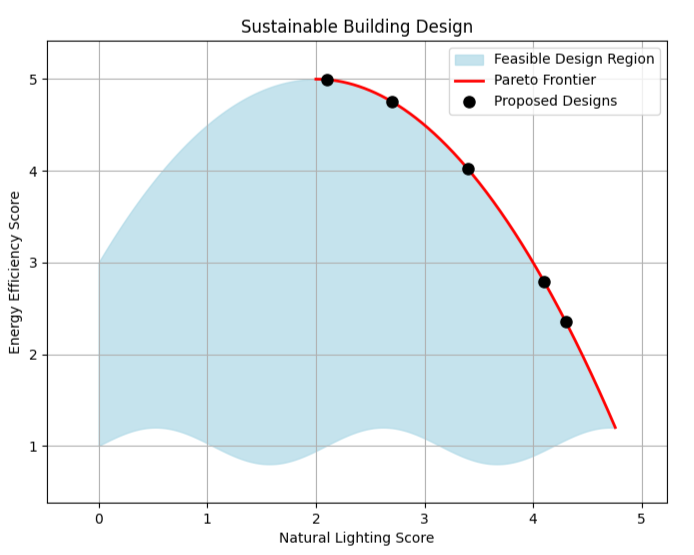
\includegraphics[width=0.6\textwidth]{ch2/figures/pareto.png}
    \caption{Pareto Frontier, feasible region and proposed designs for Sustainable Building Design}
    \label{fig:pareto_frontier}
\end{figure}

\section{Crisp MCDM Methods} \label{sec:crisp_methods}
The definitions and algorithms presented in this section are based on \cite{handbookmcdm}.\\

%Tb he leido en "lectura diagonal pag 15" sobre la clasificación en Value measurement, goal aspirations y outranking methods

\signal{From \cite{Sahoo_Goswami_2023}:}\\
\say{MCDM  methods  provide  a  systematic  and  structured framework  for  decision-making.  They  enable  decision-makers  to  break  down  complex problems  into  a  set  of  criteria,  evaluate  alternatives  against  these  criteria,  and  make informed choices based on well-defined decision rules.}
\\



% A Handbook on Multi-Attribute Decision-Making Methods, First Edition.
% Omid Bozorg-Haddad, Babak Zolghadr-Asli, and Hugo A. Loáiciga.
% © 2021 John Wiley & Sons, Inc. Published 2021 by John Wiley & Sons, Inc.

Therefore, the problem formulation usually starts by defining a decision matrix:

\begin{definition}[Decision-Matrix] 
    Let $\A =\{a_i\mid 1\leq i \leq n\} $ be the set of $n\in \N$ alternatives and $\C =\{c_j\mid 1\leq j \leq m\}$ the set of $m \in \N$ criteria. We may represent the value of the alternative $a_i$ with regard to a criterion $c_j$ as the element $d_{ij}$ of a decision-matrix $D$ as follows:
    \[D=
\setlength{\arraycolsep}{5pt} % adjust spacing if desired
\begin{array}{c@{\,}l}
  % Left block: matrix with column labels underneath
  \begin{array}{c}
    \begin{pmatrix}
      d_{11} & d_{12} & \cdots & d_{1m} \\
      d_{21} & d_{22} & \cdots & d_{2m} \\
      \vdots & \vdots & \ddots & \vdots \\
      d_{n1} & d_{n2} & \cdots & d_{nm}
    \end{pmatrix} \\[2mm] % vertical space between matrix and column labels
    \begin{array}{llll}
      \scriptstyle c_1 \hspace{1mm}& \hspace{1mm}\scriptstyle c_2 \hspace{1mm} & \hspace{1mm}\cdots  &   \hspace{1mm}\scriptstyle c_m
    \end{array}
  \end{array}
  % Right block: row labels aligned with matrix rows
  \hspace{-2.5mm}
  \begin{array}{l}
    \scriptstyle a_1 \\%[-2.5mm]
    \scriptstyle a_2 \\%[-2.5mm]
    \scriptstyle \vdots \\%[-2.5mm]
    \scriptstyle a_n\\
    \\
  \end{array}
\end{array}
\]
Where each row represents an alternative's values across all criteria, while each column shows how all alternatives perform on a single criterion.
    
\end{definition}


There is no standard classification of all the MCDM methods and there are as well mixed methods that involve ideas from a variety of them. But in order to get an approximate picture of the field, we are going to follow the classification from Belton and Stewart (2002) and see the most common methods (figure \ref{fig:MCDM_classification}):

\begin{itemize}
    \item \textbf{Value Measurement Methods:} assign each alternative a numerical value by aggregating its performance on various criteria into a single overall score, allowing for direct comparison of alternatives. They assume that all criteria can be quantified on a common scale.
    \begin{itemize}
        \item \textbf{AHP (Analytic Hierarchy Process):} Decomposes the decision problem into a hierarchical structure and uses pairwise comparisons to derive weights and scores, which are then aggregated to compute an overall value.
        \item \textbf{ANP (Analytic Network Process):} Extends AHP by accounting for interdependencies among criteria and alternatives, yet still relies on aggregating performance scores into a global value.
        \item \textbf{MAUT (Multiattribute Utility Theory):} Constructs a utility function that maps the performance of each alternative on different criteria to an overall utility value, capturing the decision maker's preferences.
    \end{itemize}
    
    \item \textbf{Goal Aspirations or Reference Level Methods:} evaluate alternatives based on their distance from pre-established ideal or reference levels. Instead of simply aggregating scores, they measure how closely each alternative meets or deviates from desired targets without requiring explicit trade-offs or weight assignments.
    \begin{itemize}
        \item \textbf{TOPSIS (Technique for Order of Preference by Similarity to Ideal Solution):} Ranks alternatives by computing their distances to both an ideal (aspiration) and an anti-ideal solution, favoring those closest to the ideal.
        \item \textbf{VIKOR (VlseKriterijumska Optimizacija I Kompromisno Resenje):}         Identifies a compromise solution by balancing the closeness of each alternative to an ideal reference point with the need to minimize regret, considering both group utility and individual dissatisfaction.
        \item \textbf{BWM (Best Worst Method):} Determines criteria weights through comparisons between the best and worst criteria against all others, thereby setting performance reference points for the evaluation.
    \end{itemize}
    
    \item \textbf{Outranking Methods:} compare alternatives pairwise to determine preference, indifference, or incomparability, leading to a ranked selection based on relative performance.
    \begin{itemize}
        \item \textbf{ELECTRE Family (Elimination and Choice Expressing Reality):}
        Uses concordance (measuring the degree of agreement) and discordance (measuring the opposition) indices in pairwise comparisons to establish if one alternative outranks another.
        \item \textbf{PROMETHEE Family (Preference Ranking Organization Method for Enrichment Evaluations):} Applies preference functions to compare alternatives pairwise, producing outranking flows that help to rank the alternatives.
    \end{itemize}
\end{itemize} 





\begin{figure}[htbp]
    \centering
    \begin{tikzpicture}[
        node distance=2cm,
        every node/.style={draw, rectangle, rounded corners, align=center, fill=blue!10, minimum width=2.5cm, minimum height=1cm},
        scale=1, transform shape
    ]
        % Root node
        \node (mcdm) {MCDM Methods};
    
        % First level: Categories arranged to the right of the root with increased vertical spacing
        \node (value) [right=3cm of mcdm, yshift=3.8cm] {Value Measurement\\Methods};
        \node (goal)  [right=3cm of mcdm] {Goal Aspirations/\\Reference Level Methods};
        \node (outrank) [right=3cm of mcdm, yshift=-3.2cm] {Outranking Methods};
    
        % Arrows from root to first-level categories
        \draw[->, thick] (mcdm) -- (value);
        \draw[->, thick] (mcdm) -- (goal);
        \draw[->, thick] (mcdm) -- (outrank);
    
        % Second level: Children of "Value Measurement Methods"
        \node (anp)  [right=2.7cm of value, yshift=1.2cm] {ANP};
        \node (ahp)  [right=2.7cm of value, yshift=0cm] {AHP};
        \node (maut) [right=2.7cm of value, yshift=-1.2cm] {MAUT};
    
        \draw[->, thick] (value) -- (anp);
        \draw[->, thick] (value) -- (ahp);
        \draw[->, thick] (value) -- (maut);
    
        % Second level: Children of "Goal Aspirations/Reference Level Methods"
        \node (topsis) [right=1.8cm of goal, yshift=1.2cm] {TOPSIS};
        \node (vikor)  [right=1.8cm of goal] {VIKOR};
        \node (bwm)    [right=1.8cm of goal, yshift=-1.2cm] {BWM};
    
        \draw[->, thick] (goal) -- (topsis);
        \draw[->, thick] (goal) -- (vikor);
        \draw[->, thick] (goal) -- (bwm);
    
        % Second level: Children of "Outranking Methods"
        \node (electre)   [right=2.5cm of outrank, yshift=0.6cm] {ELECTRE};
        \node (promethee) [right=2.5cm of outrank, yshift=-0.6cm] {PROMETHEE};
    
        \draw[->, thick] (outrank) -- (electre);
        \draw[->, thick] (outrank) -- (promethee);
    \end{tikzpicture}
    \caption{Classification of MCDM Methods following Beltan and Stewart (2002).}
    \label{fig:MCDM_classification}
    \end{figure}
    
    
    


% \subsection{Utility function methods}

% \signal{
% MAUT: ordinal utility functions and cardinal utility functions (Von Neumann-Morgenstern utility theorem)}

% \subsection{Outranking methods}
% % ===========================
% % ELECTRE I
% % ===========================
% \begin{algorithm}[H]
%     \caption{ELECTRE I Method}
%     \KwIn{Decision matrix $X=[x_{ij}]$ for $m$ alternatives and $n$ criteria, criteria weights $w_j$, concordance threshold $c^*$, discordance threshold $d^*$, and ranges $R_j$ for each criterion}
%     \KwOut{Outranking relation among alternatives and selection of the best alternatives}
%     \For{each pair of alternatives $(a,b)$}{
%         \textbf{Compute Concordance Index:}\;
%         \[
%             C(a,b) = \sum_{j \in J(a,b)} w_j, \quad \text{where } J(a,b)=\{\, j \mid x_{aj} \ge x_{bj} \,\}
%         \]\;
%         \textbf{Compute Discordance Index:}\;
%         \[
%             D(a,b) = \begin{cases}
%             \max\limits_{j \in J'(a,b)} \left( \dfrac{x_{bj}-x_{aj}}{R_j} \right), & \text{if } J'(a,b)\neq\emptyset,\\[1ex]
%             0, & \text{otherwise},
%             \end{cases}
%         \]
%         where \( J'(a,b)=\{\, j \mid x_{aj} < x_{bj} \,\}\)\;
%     }
%     \For{each pair $(a,b)$}{
%         \If{\( C(a,b) \ge c^* \) \textbf{and} \( D(a,b) \le d^* \)}{
%                 Conclude that alternative \( a \) outranks \( b \) (add an edge \( a \rightarrow b \) in the outranking graph)\;
%         }
%     }
%     Determine the kernel (set of non-dominated alternatives) or derive a ranking from the outranking graph\;
%     \Return The outranking relation and selection (or ranking) of the best alternatives\;
%     \end{algorithm}
    
% % ===========================
% % PROMETHEE II
% % ===========================
% \begin{algorithm}[H]
% \caption{PROMETHEE II Method}
% \KwIn{Decision matrix $X=[x_{ij}]$ with $m$ alternatives and $n$ criteria, criteria weights $w_j$, and parameters defining the preference functions}
% \KwOut{Complete ranking of alternatives based on net outranking flows}
% \For{each pair of alternatives $(a,b)$}{
%     \For{each criterion $j=1,\dots,n$}{
%             Compute the performance difference: 
%             \[
%             d_{j}(a,b) = x_{aj} - x_{bj}
%             \]
%             Evaluate the preference degree \( P_j(a,b) \) using the chosen preference function\;
%     }
%     Compute the aggregated preference index:
%     \[
%         \Pi(a,b) = \sum_{j=1}^{n} w_j \cdot P_j(a,b)
%     \]\;
% }
% \For{each alternative \( a \)}{
%     Compute the positive outranking flow:
%     \[
%         \phi^+(a) = \frac{1}{m-1} \sum_{b \neq a} \Pi(a,b)
%     \]\;
%     Compute the negative outranking flow:
%     \[
%         \phi^-(a) = \frac{1}{m-1} \sum_{b \neq a} \Pi(b,a)
%     \]\;
%     Compute the net flow:
%     \[
%         \phi(a) = \phi^+(a) - \phi^-(a)
%     \]\;
% }
% \Return Ranking of alternatives in descending order of \(\phi(a)\)\;
% \end{algorithm}


% \subsection{Reference point and distance-based methods}

% \begin{algorithm}[H]
%     \caption{TOPSIS Method for Multi-Criteria Decision Making}
%     \KwIn{Decision matrix $X = [x_{ij}]$ with $m$ alternatives and $n$ criteria, weights $w_j$ for each criterion}
%     \KwOut{Ranking of alternatives based on relative closeness to the ideal solution}
    
%     % Step 1: Normalize the decision matrix
%     \For{$j\leftarrow 1$ \KwTo $n$}{
%         Compute normalization factor: $d_j = \sqrt{\sum_{i=1}^{m} x_{ij}^2}$\;
%         \For{$i\leftarrow 1$ \KwTo $m$}{
%             $r_{ij} \gets \dfrac{x_{ij}}{d_j}$\;
%         }
%     }
    
%     % Step 2: Calculate the weighted normalized decision matrix
%     \For{$i\leftarrow 1$ \KwTo $m$}{
%         \For{$j\leftarrow 1$ \KwTo $n$}{
%             $v_{ij} \gets w_j \times r_{ij}$\;
%         }
%     }
    
%     % Step 3: Determine the ideal and anti-ideal solutions
%     \For{$j\leftarrow 1$ \KwTo $n$}{
%         $v_j^+ \gets \max\{v_{1j}, v_{2j}, \dots, v_{mj}\}$ \quad (if $j$ is beneficial)\;
%         $v_j^- \gets \min\{v_{1j}, v_{2j}, \dots, v_{mj}\}$ \quad (if $j$ is beneficial)\;
%         \tcp{For cost criteria, swap the definitions of $v_j^+$ and $v_j^-$}
%     }
    
%     % Step 4: Calculate separation measures for each alternative
%     \For{$i\leftarrow 1$ \KwTo $m$}{
%         $S_i^+ \gets \sqrt{\sum_{j=1}^{n} (v_{ij} - v_j^+)^2}$\;
%         $S_i^- \gets \sqrt{\sum_{j=1}^{n} (v_{ij} - v_j^-)^2}$\;
%     }
    
%     % Step 5: Calculate the relative closeness to the ideal solution
%     \For{$i\leftarrow 1$ \KwTo $m$}{
%         $C_i \gets \dfrac{S_i^-}{S_i^+ + S_i^-}$\;
%     }
    
%     % Step 6: Rank the alternatives based on $C_i$
%     \Return The alternatives ranked in descending order of $C_i$\;
%     \end{algorithm}


% % ====================================
% % 2. VIKOR Method
% % ====================================
% \begin{algorithm}[H]
%     \caption{VIKOR Method}
%     \KwIn{Decision matrix \(X = [x_{ij}]\) for \(m\) alternatives and \(n\) criteria, weights \(w_j\) for each criterion, and parameter \(v \in [0,1]\)}
%     \KwOut{Ranking of alternatives based on a compromise solution}
%     \textbf{Step 1: Determine the Best and Worst Values}\;
%     \quad \For{each criterion \(j = 1,\dots,n\)}{
%         Compute the best value: 
%         \[
%           f_j^* = \max_{i}\{x_{ij}\} \quad \text{(if maximization; use \(\min\) for minimization)}
%         \]\;
%         Compute the worst value:
%         \[
%           f_j^- = \min_{i}\{x_{ij}\} \quad \text{(if maximization; use \(\max\) for minimization)}
%         \]\;
%     }
%     \textbf{Step 2: Compute the \(S\) and \(R\) Values}\;
%     \quad \For{each alternative \(i = 1,\dots,m\)}{
%         Compute the aggregated measure:
%         \[
%            S_i = \sum_{j=1}^{n} w_j \cdot \frac{f_j^* - x_{ij}}{f_j^* - f_j^-}
%         \]\;
%         Compute the individual regret measure:
%         \[
%            R_i = \max_{j=1,\dots,n} \left[ w_j \cdot \frac{f_j^* - x_{ij}}{f_j^* - f_j^-} \right]
%         \]\;
%     }
%     \textbf{Step 3: Compute the \(Q\) Value for Each Alternative}\;
%     \quad Let 
%     \[
%     S^* = \min_{i} S_i,\quad S^- = \max_{i} S_i,\quad R^* = \min_{i} R_i,\quad R^- = \max_{i} R_i
%     \]\;
%     \quad \For{each alternative \(i = 1,\dots,m\)}{
%         Compute:
%         \[
%            Q_i = v \cdot \frac{S_i - S^*}{S^- - S^*} + (1-v) \cdot \frac{R_i - R^*}{R^- - R^*}
%         \]\;
%     }
%     \textbf{Step 4: Ranking and the Compromise Solution}\;
%     \quad Rank alternatives in ascending order of \(Q_i\)\;
%     \quad \tcp{Optionally, check for acceptable advantage and stability conditions among the top alternatives}
%     \Return Ranking of alternatives based on \(Q_i\)\;
%     \end{algorithm}



% \subsection{Pairwise comparison methods}


% % ===========================
% % ANP (Analytic Network Process)
% % ===========================
% \begin{algorithm}[H]
%     \caption{Analytic Network Process (ANP)}
%     \KwIn{A set of clusters (criteria, alternatives, etc.), pairwise comparison matrices, and information on interdependencies}
%     \KwOut{Ranking of alternatives based on final priority weights}
%     \textbf{Step 1: Network Construction}\;
%     \quad Define clusters and identify the interdependencies among them\;
%     \textbf{Step 2: Pairwise Comparisons}\;
%     \quad \For{each cluster and for each interdependency between clusters}{
%         Perform pairwise comparisons to construct local comparison matrices\;
%         Compute local priority vectors (e.g., using the eigenvector method)\;
%     }
%     \textbf{Step 3: Supermatrix Formation}\;
%     \quad Assemble all local priority vectors into the initial (unweighted) supermatrix $W$\;
%     \textbf{Step 4: Weighting the Supermatrix}\;
%     \quad Adjust $W$ by cluster weights (or inter-cluster influences) to obtain the weighted supermatrix $W'$\;
%     \textbf{Step 5: Limit Supermatrix Calculation}\;
%     \quad Raise $W'$ to a sufficiently large power until convergence, i.e., 
%     \[
%     W'^{(k)} \rightarrow W^* \quad \text{as } k \to \infty
%     \]
%     \textbf{Step 6: Derive Final Priorities}\;
%     \quad Extract the final weights for the alternatives from $W^*$\;
%     \Return Ranking of alternatives based on the final weights\;
%     \end{algorithm}


% % ====================================
% % 1. Analytic Hierarchy Process (AHP)
% % ====================================
% \begin{algorithm}[H]
%     \caption{Analytic Hierarchy Process (AHP)}
%     \KwIn{A set of criteria and alternatives, pairwise comparison matrices for criteria and for alternatives under each criterion}
%     \KwOut{Final ranking of alternatives based on global priorities}
%     \textbf{Step 1: Hierarchy Construction}\;
%     \quad Define the goal, criteria, and alternatives\;
%     \textbf{Step 2: Pairwise Comparison of Criteria}\;
%     \quad Construct the pairwise comparison matrix for the criteria\;
%     \quad Compute the eigenvector of this matrix to obtain criteria weights \(w_j\)\;
%     \quad \tcp{Optionally check the consistency ratio for reliability}
%     \textbf{Step 3: Pairwise Comparison of Alternatives}\;
%     \quad \For{each criterion \(j = 1,\dots,n\)}{
%         Construct the pairwise comparison matrix for the alternatives with respect to criterion \(j\)\;
        
%         Compute the eigenvector for this matrix to obtain local priorities \(p_{ij}\) for each alternative \(i\) under criterion \(j\)\;
        
%         \tcp{Optionally check the consistency ratio for each matrix}
%     }
%     \textbf{Step 4: Global Priority Synthesis}\;
%     \quad For each alternative \(i\), compute the global priority:
%     \[
%     P_i = \sum_{j=1}^{n} w_j \cdot p_{ij}
%     \]
%     \Return Ranking of alternatives based on the global priorities \(P_i\)\;
%     \end{algorithm}




\section{Assigning membership values (fuzzification).}
Fuzzy sets, as discussed in chapter \ref{ch:intro}, provide a way to encode data. In the case of MCDM  problems, we are particularly interested in modeling the vagueness of fuzzy attributes. And as stated in section \ref{sec:fuzzy_sets} with the set of \emph{tall people}, there is not a unique way to define the membership value of an object to a fuzzy set.\\

Information from three key sources is often considered to define membership functions, and we may exemplify them through the same case of people's height mentioned above: First, concept-driven constraints arise from the inherent nature of what is being modeled (higher heights do not correspond to ''less tall"). Second, domain knowledge or data provides empirical foundations, such as population height statistics, height requirements for particular activities (like basketball), or expert knowledge (the judgement of a basketball coach). Third, the preferences of the decision maker shape the final form, reflecting aspects such as their risk tolerance and the desired level of discrimination between alternatives.\\

The inherent variability in constructing membership functions naturally leads to a fundamental question: how critical is the exact shape of a fuzzy set to the final outcome? Fortunately, for many of the logical operations used in decision-making models, the system's output is not overly sensitive to minor perturbations in the input membership functions. This robustness implies that while the general form of the function is important, the precise membership values are often less critical than they might appear \cite{ExactFuzzySetShape}.\\

The process of defining these membership functions is known as fuzzification. Since it is a crucial first step in any fuzzy logic application, the following subsections explore membership function construction methods, which are broadly categorized according to the source of information: elicitation from domain experts, learning from empirical data, or derivation from other pre-existing fuzzy sets.

\subsection{Elicitation from Domain Experts}
An approach to construct membership functions when empirical data is scarce, or the concept being modeled is highly subjective, is to elicit information from domain experts. This process, which can be performed through direct or indirect methods, leverages human knowledge and intuition to quantify vague concepts.

\paragraph{Direct Elicitation}
The most straightforward method is direct elicitation, where an expert is asked to directly assign a numerical membership grade to a series of elements in the universe of discourse. For example, to define the fuzzy set for \emph{high temperature} in a room, the expert could be polled to provide a value between 0 and 1 for several different temperatures. These results form a set of points that define the membership function. For continuous fuzzy sets or cases with too many surveyed points, this approach becomes infeasible. A key consideration is the scale used for elicitation, which can then be mapped into the $[0,1]$ interval. A common strategy is to use $7\pm2$ categories when making absolute judgements along a single dimension. This idea originated in a psychology paper \cite{miller1956magical}, suggests that simpler scales may be more appropriate than finer ones for elicitation tasks.

\paragraph{Indirect and Compositional Elicitation}
A more interpretable and often more robust approach is indirect elicitation, which avoids requiring experts to provide precise values for each element and instead employs parametrized functional forms. This is commonly achieved through the use of linguistic variables, which provide a formal structure for handling verbal concepts.

\begin{definition}[Linguistic Variable \cite{Zadeh1975}]
A \textbf{linguistic variable} is a variable (e.g., \emph{age}) whose values are words or sentences rather than numbers. It is characterized by a set of linguistic values, or \textbf{terms} (e.g., \emph{young}), defined over an underlying numerical \textbf{base variable} (e.g. a numerical variable \texttt{x} whose values are the integers from 0 to 100). The meaning of each term is captured by a fuzzy set, whose membership function (compatibility function), specifies the degree to which any value on the base variable is compatible with the linguistic label.
\end{definition}

Instead of defining this compatibility function point-by-point, an expert can specify it by choosing a standard, parameterized shape that is easy to interpret. For instance, a triangular fuzzy number is intuitive for representing a concept centered ``around" a certain point, while a trapezoidal shape can represent a concept that is fully valid over an interval. 

Furthermore, new linguistic values can be derived compositionally from existing ones using \emph{linguistic modifiers}, or hedges. These are operations that alter a membership function, such as concentrators like \emph{very}, which makes a fuzzy set more specific, and dilators like \emph{somewhat}, which makes it less specific. These effects are often achieved by applying an exponent to the original membership function: f
or a concentrator like \emph{very}, the membership values are raised to an exponent greater than 1 (e.g. $\mu_{\text{very } A}(x) = (\mu_A(x))^2$), while for a dilator like \emph{somewhat}, an exponent between 0 and 1 is used (e.g. $\mu_{\text{somewhat } A}(x) = \sqrt{\mu_A(x)}$).

\begin{example}
    Consider the linguistic variable \emph{Price}. An expert might define the term \emph{cheap} as being fully true for prices below 30\euro$\,$ and completely false above 70\euro. Similarly, the term \emph{expensive} could be defined as false below 50\euro$\,$ and fully true above 90\euro. 
    
    This formulation creates an overlap region (between 50\euro$\,$ and 70\euro) where an item can be considered, to some degree, \emph{both} cheap and expensive, capturing the inherent ambiguity of mid-range pricing. From these base terms, modifiers like \emph{very} and \emph{somewhat} are used to derive more nuanced linguistic values, as illustrated in Figure \ref{fig:linguistic_variable_overlap}.
\end{example}

\begin{figure}[!ht]
    \centering
    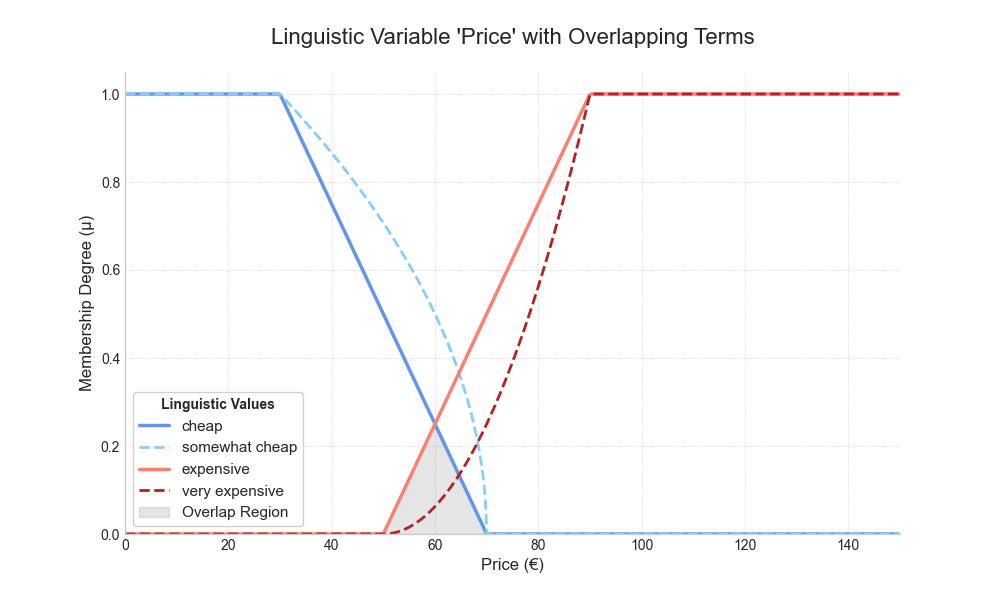
\includegraphics[width=0.8\textwidth]{ch2/figures/fuzzy_var_car_example.png}
    \caption{An illustration of the linguistic variable 'Price' with overlapping terms. The overlap between 'cheap' and 'expensive' represents the ambiguity of mid-range prices. Modifiers create more specific or general terms.}
    \label{fig:linguistic_variable_overlap}
\end{figure}


\subsection{Learning from Data}
When relevant data is available, membership functions can be constructed through learning algorithms. This approach frames the task as an optimization problem, where the goal is to find the membership function that best fit the available data.\\

In a supervised learning context, we have a dataset of input-output pairs. For example, consider a company with data regarding products (e.g. their characteristics) and customer satisfaction surveys. Each product would be an element of the universe and its membership grade is derived from the satisfaction surveys. We can then use function approximation techniques (e.g. Machine Learning models like artificial neural networks), to learn a membership function from the data and use them to generalize to new products with similar characteristics without needing to survey them.\\

In many real-world scenarios, however, we do not have such input-output pairs. For these unsupervised learning contexts, several approaches could be employed, such as fuzzy clustering (which is implemented in the next chapter). This algorithm partitions a dataset into several groups, allowing each data point to belong to multiple clusters with varying degrees of membership. These membership degrees can then be interpreted as the values of the membership function for the fuzzy set represented by each cluster. The Fuzzy C-Means (FCM) algorithm \cite{bezdek1984fcm} stands as the most widely used method in this category.

\paragraph{Fuzzy C-Means (FCM) algorithm} Given a dataset $X = \{x_1, x_2, \ldots, x_n\}$ of $n$ data points in an $r$-dimensional space, FCM aims to find a partition of $X$ into $c$ fuzzy clusters by minimizing the objective function:
\[
J_m(U, V) = \sum_{i=1}^{c} \sum_{k=1}^{n} (u_{ik})^m \|x_k - v_i\|^2
\]
where $U$ is the partition matrix with elements $u_{ik}$ representing the membership of data point $x_k$ in cluster $i$, $V = \{v_1, \ldots, v_c\}$ is the set of cluster centers, and $m > 1$ is a fuzzification parameter that controls the degree of cluster overlap. The minimization of $J_m$ is performed iteratively through the following steps:
\begin{enumerate}
    \item Initialize the partition matrix $U^{(0)}$ randomly, subject to $\sum_{i=1}^{c} u_{ik} = 1$ for each $k$.
    \item At iteration $t$, calculate the cluster centers $V^{(t)}$:
    \[
    v_i^{(t)} = \frac{\sum_{k=1}^{n} (u_{ik}^{(t-1)})^m x_k}{\sum_{k=1}^{n} (u_{ik}^{(t-1)})^m}
    \]
    \item Update the partition matrix $U^{(t)}$:
    \[
    u_{ik}^{(t)} = \left( \sum_{j=1}^{c} \left( \frac{\|x_k - v_i^{(t)}\|}{\|x_k - v_j^{(t)}\|} \right)^{\frac{2}{m-1}} \right)^{-1}
    \]
    \item Repeat steps 2 and 3 until the change in the partition matrix, $\|U^{(t)} - U^{(t-1)}\|$, is smaller than a predefined threshold.
\end{enumerate}
Once the algorithm converges, the resulting column $i$ of the matrix $U$ can be taken as the membership function for the fuzzy set represented by cluster $i$.\\

Memberships decay with the exponent ${-2/(m-1)}$, which provides key insights into the algorithm's operation. When $m$ approaches 1, the exponent approaches negative infinity, causing the nearest center to dominate and resulting in nearly crisp labels. Conversely, as $m$ approaches infinity, the exponent approaches 0, causing distances to lose influence and all memberships to converge to $1/c$. This behavior is clearly illustrated in Figure \ref{fig:fuzzy_cmeans}, which shows how different values of $m$ affect the clustering results.

\begin{figure}[!ht]
    \centering
    \begin{adjustwidth}{-1.7cm}{-1cm}
    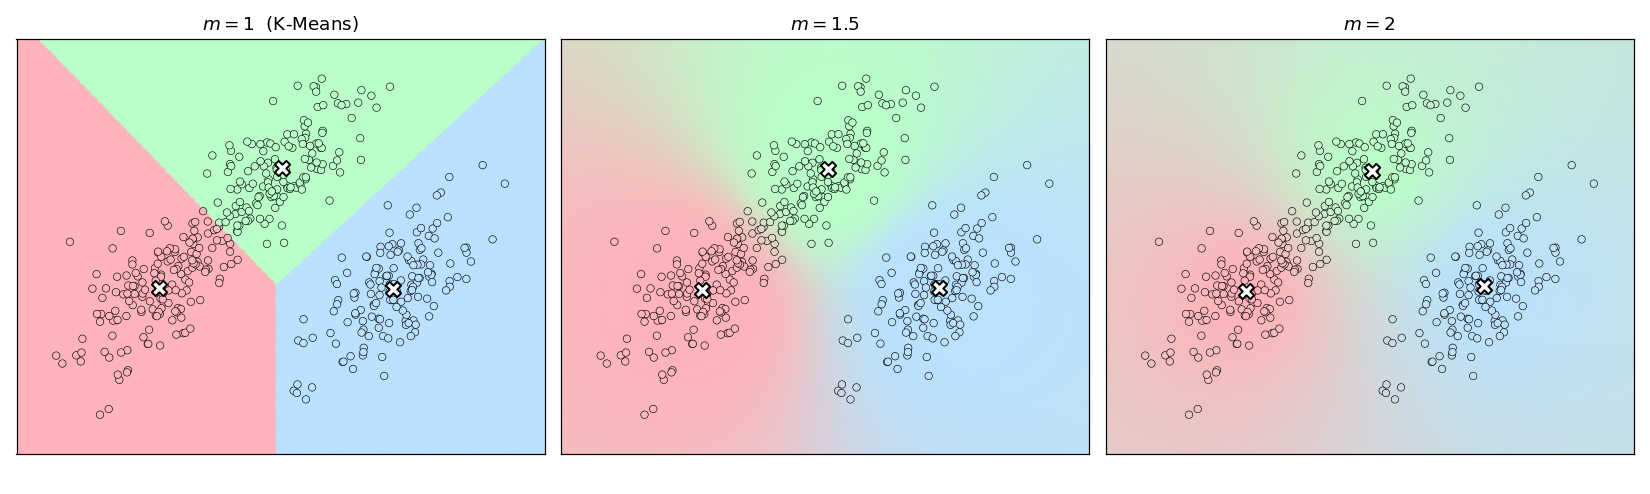
\includegraphics[width=1.15\textwidth]{ch2/figures/fuzzy_cmeans.png}
\end{adjustwidth}
    \caption{3 plots of fuzzy cmeans for 3 clusters with different m values (1, 1.5 and 2). Each color correspond to a cluster whose center is marked with the white cross. Memberships are denoted using gradients of color, where fainter tones denote lower membership values.}
    \label{fig:fuzzy_cmeans}
\end{figure}

\begin{example}
    A marketing firm could use FCM to segment customers based on their purchasing habits (e.g., purchase frequency and average transaction value). The algorithm might identify three clusters, like \emph{Low-Value}, \emph{Medium-Value}, and \emph{High-Value} customers. The membership value $u_{ik}$ would represent the degree to which customer $k$ belongs to the \emph{High-Value} fuzzy set, providing a more nuanced classification than a crisp assignment.
\end{example}

\subsection{Deriving from Other Fuzzy Sets}
New fuzzy sets can also be constructed from existing ones. The most common method is the use of fuzzy set operations (intersection, union and complement), which are particularly useful for creating complex fuzzy concepts from simpler, elementary ones. For instance, if we have already defined membership functions for the fuzzy sets \emph{cheap cars} and \emph{comfortable cars}, we can derive the membership function for \emph{cheap and comfortable cars} by applying a fuzzy AND operator (a t-norm) to the membership values of the original sets.\\

Another, more complex, method involves the use of fuzzy relational equations \cite[Sec.~3.5]{HistoryFL2017}. This approach is typically formulated as an inverse problem. A fuzzy relational equation describes a relationship between two or more fuzzy variables, often in the form $R = P \circ Q$, where $P$ and $Q$ are fuzzy relations and $\circ$ is a composition operator. If two of the three components are known, the third can be determined by solving the equation.

\begin{example}
    In medical diagnosis, let $S$ be a fuzzy relation between patients and symptoms, and $D$ be a fuzzy relation between patients and diseases. These two may be linked through a fuzzy relation $K$ representing medical knowledge, such that $D = S \circ K$. If we have observed data for patients' symptoms $S$ and their final diagnoses $D$, we could solve this equation to infer the underlying medical knowledge relation $K$ that connects symptoms to diseases.
\end{example}
\section{Fuzzy Aggregation}\label{sec:fuzzy_aggregation}
Para qué usamos en el MDCM el fuzzy? Para manejar Uncertainty y subjectivity.

Information integration (aggregation)

Distance measures

Preference relations


\signal{OWA operators, y sus generalizaciones. Orness, andness, orlike y andlike.

Entropía de un OWA, quantifiers

Fuzzy implication operators para la importancia de los OWA

Fuzzy ratings, que es como tener 2 fuzzy weights y así incorporas la linguistic variable.

Fuzzy reasoning: tienes fuzzy rules y las agregas con un OWA por ejemplo. Puedes hacer la implicación y luego agregar o agregar y luego hacer la implicación.

MICA operators es la clase más general de operators en fuzzy modeling.

3 mecanismos de MISO fuzzy system

Compositional rule of inference

Generalized method of case inference rule

Interdependencia de los criterios!}


% \section{Fuzzy Preference Relations}
% \signal{Crea fuzzy additive preference relation o fuzzy multiplicative preference relation con lo que saca una judgement matrix en lugar de la decision matrix. Esto puede implementarse en algoritmos tipo AHP.}
% \section{Fuzzy Measure}

% \signal{Entropy measures o correlation measures para hacer un fuzzy clustering. También distance/similarity based measures between fuzzy elements para un fuzzy TOPSIS}

% \section{Other Approaches}
% \signal{Y si entendemos concepts como fuzzy sets, entonces buscamos relaciones entre concepts como fuzzy subsets (equiv fuzzy implications?) con un algoritmo tipo clustering y eso nos da información sobre los criterios que tenemos y cómo evalúan para cada alternative?\\
This way, we say that “$A$ is a fuzzy subset of $B$” if and only if

$I(\mu_A(x), \mu_B(x)) = 1$ for every $x$

And we can relax that condition to approximate fuzzy subset. Esto creo que se ha hecho ya con probabilistic reasoning.\\

Esto me recuerda mucho a lo que decía en Rough Sets y lo del trabajo de dominance based rough sets approach (DRSA) igual tiene ideas que se pueden llevar aquí. También estaba por ahí lo de DRSA con fuzzy para la inducción de reglas, eso puede estar muy bien.} 
% \chapter{Case Study: A Fuzzy Multi-Criteria Decision Analysis}\label{ch4}


The problem that will be tackled in this chapter is the ROADEF/EURO Challenge 2020: Maintenance Planning Problem \cite{roadef2020}, which was jointly organized by the French Operational Research and Decision Support Society (ROADEF) and the European Operational Research Society (EURO) in collaboration with RTE (Réseau de Transport d'Électricité).\\

The ROADEF/EURO Challenge is a prestigious biennial competition that bridges the gap between academia and industry by inviting researchers to tackle complex, real-world optimization problems. The 2020 edition was motivated by operational necessity and strategic foresight in the energy sector: while preventive maintenance is essential for grid reliability, the act of taking a power line out of service temporarily weakens the network, increasing its vulnerability to unexpected contingencies like extreme weather or other equipment failures. This challenge has become significantly more complex due to the energy transition. The increasing integration of intermittent renewable energies creates new operational dynamics and constraints, making traditional planning methods insufficient. RTE had already developed a unique strategy to quantify the financial risks of every potential maintenance task across thousands of future scenarios. The core purpose of the challenge was to invite the world's top researchers to develop a powerful optimization engine for the second, most complex step of this process: using this massive, pre-calculated risk data to build a feasible and robust annual maintenance schedule.\\

The competition was organized in a systematic multi-phase structure to identify optimal solutions from an international pool of participants. A total of 74 teams from over 20 countries participated across junior (pre-PhD) and senior tracks. The competition proceeded through three main phases, with each phase utilizing different sets of 15 problem instances representing different maintenance planning scenarios. The qualification phase required teams to submit solutions for a public instance set (Set A), with the top 15 teams advancing based on a point-per-instance scoring system. In the semi-final phase, qualified teams tackled a larger instance set (Set B), resulting in 13 finalists (10 senior and 3 junior). The final phase challenged teams with both a known set (Set C) and a hidden set (Set X) of instances. Final rankings were determined through two distinct evaluation runs on the organizers' machines: a 15-minute "fast score" run and a decisive 90-minute "quality score" run. The winner was ultimately announced at the EURO 2021 conference. \\


The competition employed a progressive evaluation methodology utilizing increasingly complex instances to assess algorithm effectiveness and scalability. For our purposes, instance difficulty was quantified through objective function scores. The X dataset comprised the most challenging problems, characterized by significant risk penalties during peak demand periods. Therefore, instance \texttt{X12} was selected for detailed analysis despite having only the second-highest objective score after \texttt{X14} which achieved the highest score. The reason is that it demonstrated greater improvement between the 15-minute and 90-minute computational runs. This behavior indicates that extended computation times could generate more diverse scheduling alternatives for our multi-criteria optimization problem.


\section{ Original Problem Description}
The maintenance planning problem aims to schedule the starting times of a set of interventions (i.e., maintenance tasks) over a time horizon (typically one year, discretized into days or weeks). The goal is to minimize risk-related costs represented as a single objective function \ref{eq:objective}, while satisfying resource and exclusion constraints. 
This is formalized in table \ref{tab:variables} and as an integer programming optimization problem (following the description from \cite{ConsueloRoadef}):\\


\begin{table}[h]
  \centering
  \begin{tabular}{|c|p{13cm}|}
    \hline
    \textbf{Symbol} & \textbf{Description} \\ \hline
    $T$ & Total number of time periods in the planning horizon. \\ \hline
    $t$ & Time period index, with $t \in \{1,\ldots,T\}$. \\ \hline
    $\tau$ & Starting time period for interventions, with $\tau \in \{1,\ldots,T\}$. \\ \hline
    $I$ & Set of interventions. \\ \hline
    $x_{i,\tau}$ & Binary variable: 1 if intervention $i\in I$ starts at period $\tau$, 0 otherwise. \\ \hline
    $d_{i,\tau}$ & Duration of intervention $i$ if started at period $\tau$. \\ \hline
    $C$ & Set of resources (teams). \\ \hline
    $l_{c,t},\, u_{c,t}$ & Lower and upper bounds on the availability of resource $c\in C$ at period $t$. \\ \hline
    $r_{c,t}(i,\tau)$ & Consumption of resource $c$ in period $t$ by intervention $i$, if started at $\tau$. \\ \hline
    $\mathcal{E}$ & Set of exclusion triplets $(i_1,i_2,t)$ (interventions $i_1,i_2$ cannot overlap at $t$). \\ \hline
    $S_t$ & Set of scenarios for period $t$. \\ \hline
    $\mathrm{risk}_{s,t}^{(i,\tau)}$ & Risk cost in scenario $s\in S_t$ for intervention $i$ (if started at $\tau$) during period $t$. \\ \hline
    $\alpha$ & Weight in the objective, with $\alpha\in[0,1]$. \\ \hline
  \end{tabular}
  \caption{Main Variables and Parameters}
  \label{tab:variables}
\end{table}

\vspace{1em}


\noindent\textbf{Objective:}
\begin{equation}
\min \; \alpha\,\mathrm{obj}_1 + (1-\alpha)\,\mathrm{obj}_2(\beta) \qquad \text{ with }\alpha \in [0,1]
\label{eq:objective}
\end{equation}
where
\[
\begin{aligned}
&\mathrm{obj}_1 = \frac{1}{T}\sum_{t=1}^{T} \mathrm{risk}_t,\quad \mathrm{obj}_2(\beta) = \frac{1}{T}\sum_{t=1}^{T} \max\Big\{0,\;Q_t^\beta-\mathrm{risk}_t\Big\},\\[1ex]
&\quad\text{with: }\quad\mathrm{risk}_t = \frac{1}{|S_t|}\sum_{s\in S_t}\sum_{\substack{i\in I\\ \tau \le t < \tau+d_{i,\tau}}} \mathrm{risk}_{s,t}^{(i,\tau)}\,x_{i,\tau},\quad Q_t^\beta=\beta\text{-quantile of } \Big\{\mathrm{risk}_{s,t} : s\in S_t\Big\}.
\end{aligned}
\]
\noindent Here, $\mathrm{obj}_1$ is the mean cumulative planning risk and $\mathrm{obj}_2(\beta)$ quantifies the extremely high-risk scenarios and periods we want to avoid.

\vspace{1em}
\noindent\textbf{Subject to:}

\noindent Each intervention is scheduled exactly once:
\[
\sum_{\tau=1}^{T-d_{i,\tau}+1} x_{i,\tau} = 1,\quad \forall\, i\in I
\]

\noindent Intervention finishes within the horizon:
\[
t + d_{i,\tau} \le T+1,\quad \forall\, i\in I \text{ and } t \text{ with } x_{i,\tau}=1
\]

\noindent Resource capacity limits:
\[
l_{c,t} \le \sum_{i\in I}\sum_{\tau \le t < \tau+d_{i,\tau}} r_{c,t}(i,\tau)\,x_{i,\tau} \le u_{c,t},\quad \forall\, c\in C,\; \forall\, t
\]

\noindent Exclusion constraints:
\[
\sum_{\tau:\, t\in [\tau,\,\tau+d_{i_1,\tau}-1]} x_{i_1,\tau} + \sum_{\tau:\, t\in [\tau,\,\tau+d_{i_2,\tau}-1]} x_{i_2,\tau} \le 1,\quad \forall\,(i_1,i_2,t)\in \mathcal{E}
\]

\noindent Binary variables:
\[
x_{i,\tau} \in \{0,1\},\quad \forall\, i\in I,\; \tau=1,\ldots,T-d_{i,\tau}+1
\]



\section{Building the Decision Matrix}
The presented optimization problem employs binary decision variables and a single aggregated objective function with crisp parameter values to provide a clear, tractable, and straightforward formulation. Such a representation is very practical due to its computational efficiency, interpretability, and ease of implementation using standard optimization solvers. However, this framework neglects the uncertainty, imprecision, and conflicting nature of  real-world criteria, such as varied stakeholder preferences, uncertain resource availability, or imprecise risk estimations. Some of these aspects are precisely what we aim to model in this chapter to help a single decision maker select a specific schedule from a pool of feasible solutions. \\

The following section provides a detailed explanation of how the decision matrix (see table \ref{tab:dm_matrix}) is obtained by defining their attributes and explaining how different schedules (solutions) were computed using 3 of the top performing algorithms from the competition.

\subsection{Alternative Generation}

The analysis evaluates a pool of alternative schedules obtained from three leading algorithms submitted to the Roadef2020 challenge. These algorithms were selected from among the 13 finalists as they were the only ones that had their compiled solution code publicly available. These top performing solutions include the overall winning algorithm by Buljubašić and Vasquez\cite{top1} (Team S34) which secured first place, the matheuristic by Parreño et~al.\cite{ConsueloRoadef} (Team S56) which ranked third overall, and the algorithm by Marco Langiu\cite{top5} (Team J73) which won the junior category and ranked fifth overall.\\



The winning algorithm (S34) employs a scenario-penalisation matheuristic, which begins by solving a relaxed version of the problem with low penalties for constraint violations. It then iteratively increases these penalties, gradually guiding the search from initially cheap but infeasible solutions towards high-quality, feasible ones. The third-place solution (S56) follows a structured three-phase pipeline: it first generates multiple diverse schedules using a randomized greedy construction, refines them with a systematic local search, and finally uses an exact solver to optimally re-plan only the most critical activities. In contrast, the junior-winning algorithm (J73) relies almost entirely on a single mathematical model (Mixed-Integer Linear Programming), with its competitiveness stemming from a very effective greedy heuristic used to generate a high-quality initial solution to dramatically accelerate the exact solver.\\

Each algorithm was ran on the instance \texttt{X12} with different maximum computation times (180s, 300s, 500s, 700s, and 900s) and three different random seeds (42, 33, 73) on a GIGABYTE AORUS 15 BSF laptop with a 13th Gen Intel Core i7-13700H CPU and 16GB of DDR5-4800 RAM. This amounts to a total of 45 solutions (15 solutions per algorithm). However, the algorithm from Langiu failed to find feasible solutions in 4 of the setups, leaving a total of 41 solutions. The heat map (figure \ref{fig:dif_sol}) reveals that solutions 30-41 contain identical intervention schedules. Since these represent repeated solutions, only one representative (solution 30) will be kept, leaving us with 29 distinct solutions for analysis.

\begin{figure}[ht]
    \centering
    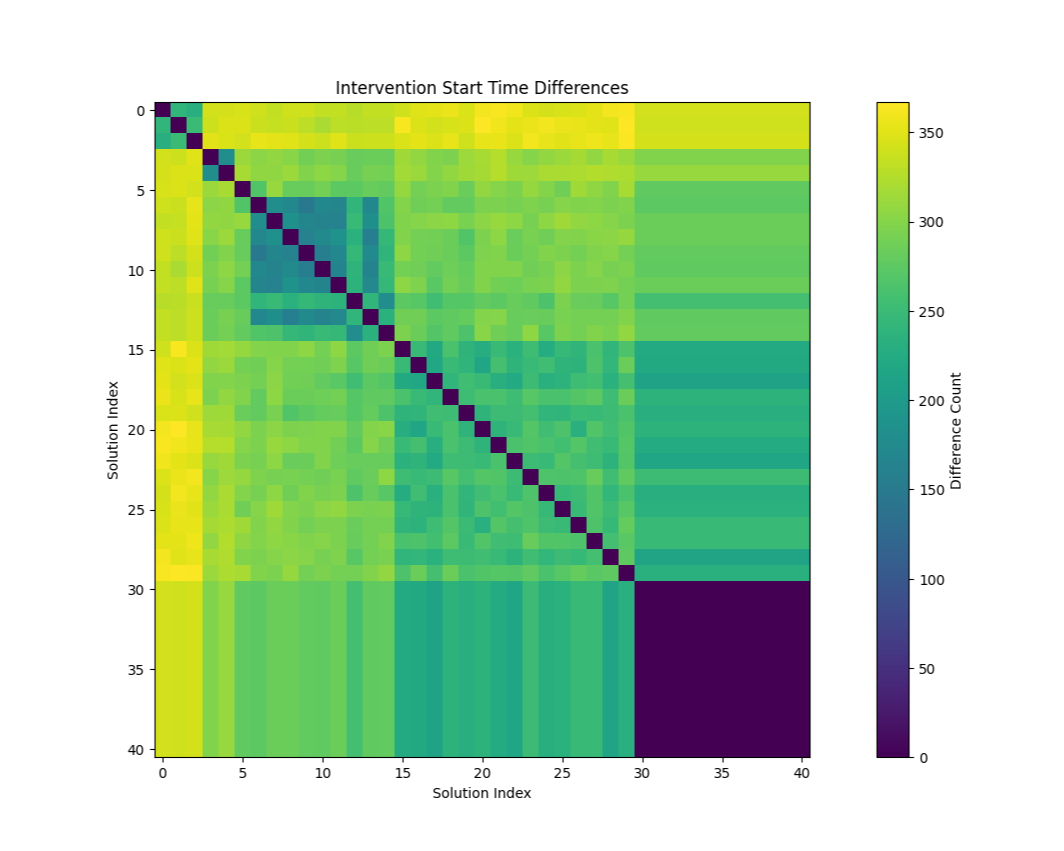
\includegraphics[width=0.8\textwidth]{ch3/figures/diff_sol.png}
    \caption{Heat map showing the count of different scheduled interventions between each pair of solutions. Solutions 30-41 are identical and correspond to the algorithm from Langiu.}
    \label{fig:dif_sol}
\end{figure}




\subsection{Retriving the physical location of the interventions}
One of the assumptions that will be made is that there is a component of the risk that comes from the location of an intervention. This is intuitive since interventions in densely populated areas or near critical infrastructure likely carry higher risks than those in remote locations. However, location is not the only factor, the risk also depends on other variables like the type of maintenance work. \\

Therefore, we will attempt to infer the approximate location of the interventions stating the following:
\begin{notation}{Assumption 1:}
    Two interventions \(i\) and \(j\) are close, for all time periods, their overall mean risks (averaged accross all possible start times and scenarios)
    \[
    \overline{r}_t^{(i)} = \frac{1}{\left|\mathcal{T}_i\right|}\sum_{\mathcal{T}_i}\mu_t^{(i,\tau)}, 
    \qquad \text{where }\mu_t^{(i,\tau)} \coleq \frac{1}{|S|}\sum_{s\in S} \mathrm{risk}_{s,t}^{(i,\tau)}, \quad
    \mathcal{T}_i\coleq \{\tau\in \N:\,1\leq \tau \leq T-d_{i,\tau}\}
    \]
    vary in the same direction, i.e.,
    \[
    \operatorname{sgn}\Big(\overline{r}_{t+1}^{(i)}-\overline{r}_t^{(i)}\Big)=\operatorname{sgn}\Big(\overline{r}_{t+1}^{(j)}-\overline{r}_t^{(j)}\Big)\quad\forall t\in\{1,\dots , T\}
    \]
    This affirms that the risk variation of an intervention over time is strongly correlated with its location.
    \end{notation}


In practice, this crisp equivalence relation will rarely hold for all time periods $t$. However, we can use it to define a similarity measure between interventions by counting how often their risk variations align. Specifically, for each pair of interventions $(i,j)$, we compute a similarity score by adding 1 when their risk variations match in sign and subtracting 1 when they differ. Then it is normalized to the interval $[-1,1]$. This yields a symmetric similarity matrix that captures the degree of correlation between intervention risks over time.

\begin{remark}
    By definition, an intervention has a correlation of 1 with itself.
\end{remark}

Notice that not all correlation values provide information about the closeness between interventions. Only positively correlated interventions can be considered "close" to some extent. However, we cannot determine how far apart negatively correlated interventions should be. Therefore, these negative correlations will be set to \texttt{NaN} and treated as missing values.\\

There is not enough information to assign a specific distance value between 2 close points, but following assumption 1: the higher the correlation between two interventions, the stronger the indication that they are close to each other. Therefore, the algorithm proposed to recover a map from a distance matrix is: non-metric weighted Multi-Dimensional Scaling (MDS):

\begin{itemize}
    \item \textbf{MDS:} Given a distance matrix (or dissimilarity matrix), it minimizes a stress function (\ref{eq:stress}) to find an embedding in a specified number of dimensions (in our case, 2 dimensions).
    \item \textbf{Non-metric:} Instead of using the magnitude of the distances, it only considers the ordinal information induced by those values. Higher correlations indicate closer distances, but the size of the difference between correlations is not necessarily proportional to the actual distances between interventions.
    \item \textbf{Weighted:} Each distance's contribution to the stress function is weighted by its correlation value, reflecting higher confidence in our assumption when correlations are stronger.
\end{itemize}

\begin{remark}
    The dissimilarity/distance matrix is obtained through a linear transformation of the previously defined similarity matrix:
    \begin{align*}
        \text{NaN} &\rightarrow \text{NaN} \\
        \text{cor}_{ij} &\rightarrow \text{dist}_{ij} = 1-\text{cor}_{ij}, \quad \text{where } \text{cor}_{ij} \in [0,1]
    \end{align*}
\end{remark}


\subsubsection*{Non-metric Weighted MDS with SMACOF:}
\paragraph{Problem Formulation .} Let us assume we have $n$ objects, and an $n\times n$ matrix of observed dissimilarities 
\[
\Delta = \bigl[\delta_{ij}\bigr],
\]
where $\delta_{ij} \ge 0$ and each pair of objects $(i,j)$ is assigned a weight $w_{ij}\ge 0$. The goal of \emph{non-metric} weighted MDS is to find an embedding of these objects as points $\mathbf{x}_1,\dots,\mathbf{x}_n$ in $\mathbb{R}^p$ (collectively denoted by $X \in \mathbb{R}^{n\times p}$), such that the pairwise distances $d_{ij}(X) = \|\mathbf{x}_i - \mathbf{x}_j\|$ (usually Euclidean) respect the \emph{rank ordering} of $\delta_{ij}$.

Formally, non-metric MDS replaces $\delta_{ij}$ with a \emph{monotonic transformation} $f(\cdot)$, yielding
\[
\hat{\delta}_{ij} = f(\delta_{ij}),
\]
subject to the isotonic constraint:
\[
\delta_{ij} < \delta_{kl} 
\quad \Longrightarrow \quad 
f(\delta_{ij}) \;\le\; f(\delta_{kl}).
\]
In case of a tie $(\delta_{ij} = \delta_{kl} )$, disparities are allowed as long as they maintain the correct ordering with respect to non-tied values.

We then define the \emph{weighted STRESS} function:
\begin{equation}
\mathrm{STRESS}(X,\hat{\Delta}) 
\;=\;
\sum_{i<j} w_{ij}\,\bigl(\hat{\delta}_{ij} \;-\; d_{ij}(X)\bigr)^2,
\label{eq:stress}
\end{equation}
where $\hat{\Delta}$ denotes the matrix $\bigl[\hat{\delta}_{ij}\bigr]$.  
The goal is to minimize this STRESS with respect to both $X$ and the (monotonic) mapping $f$. Missing values are simply not taken into account in the sum (which is equivalent to setting their weight to 0).

\paragraph{Solution via SMACOF \cite{smacof}}\label{sec:smacof-solution}
\emph{Scaling by MAjorizing a COmplicated Function} is an iterative algorithm that provides a stable, monotone-convergent framework for MDS. Unlike Kruskal's classic method, which uses gradient-based updates to move the configuration $X$, SMACOF replaces the gradient step with a \emph{majorization step} that guarantees non-increasing STRESS accross iterations. This is typically more numerically stable and better at handling large amounts of missing data.

The algorithm alternates between two main steps:

\begin{enumerate}
  \item \textbf{Initialization}
    \begin{enumerate}[(a)]
      \item Collect all non-missing dissimilarities $\{\delta_{ij}\}$ and set the corresponding weights $w_{ij}$ (with $w_{ij}=0$ for missing values).
      \item Choose an initial configuration $X^{(0)} \in \mathbb{R}^{n \times p}$ (e.g., via random placement or classical MDS).
    \end{enumerate}

  \item \textbf{Iterative Steps}
    \begin{enumerate}[(a)]
      \item \textbf{Optimal Scaling (Isotonic Regression):} \\
      Given the current configuration $X^{(t)}$, compute the Euclidean distances
      \[
        d_{ij}\bigl(X^{(t)}\bigr)=\|x_i^{(t)} - x_j^{(t)}\|,
      \]
      and determine the disparities by solving
      \[
        \min_{f\,:\, \text{non-decreasing}} \sum_{i<j} w_{ij}\,\Bigl(f(\delta_{ij}) - d_{ij}\bigl(X^{(t)}\bigr)\Bigr)^2.
      \]
      In practice, weighted isotonic regression (e.g., via the Up-and-Down-Blocks Algorithm \ref{algo:Up-and-Down-Blocks}) is applied to obtain $\hat{\delta}_{ij}=f(\delta_{ij})$, ensuring that the transformed dissimilarities preserve the original rank order.
      
      \item \textbf{Majorization Update (Guttman Transform):} \\
      With the disparities $\hat{\Delta}=\{\hat{\delta}_{ij}\}$ fixed, 
      SMACOF constructs a quadratic majorizing function $Q\bigl(X, X^{(t)}\bigr)$ satisfying
      \[
        \mathrm{STRESS}(X,\hat{\Delta}) \le Q\bigl(X, X^{(t)}\bigr), \quad \text{with equality when } X = X^{(t)}.
      \]
      Minimizing $Q$ leads to a closed-form update via the Guttman transform:
      \[
        X^{(t+1)} = V^{+}B\bigl(X^{(t)}\bigr)X^{(t)},
      \]
      where the matrix $B\bigl(X^{(t)}\bigr)$ is defined element-wise by
      \[
        B_{ij}\bigl(X^{(t)}\bigr)=
          \begin{cases}
            -\dfrac{w_{ij}\,\hat{\delta}_{ij}}{d_{ij}\bigl(X^{(t)}\bigr)} & \text{if } i\neq j, \\[1mm]
            -\displaystyle\sum_{k\neq i} B_{ik}\bigl(X^{(t)}\bigr) & \text{if } i = j,
          \end{cases}
      \]
      and $V$ is a constant matrix determined by the weights (its Moore-Penrose inverse is denoted $V^{+}$). By construction, the update satisfies
      \[
        \mathrm{STRESS}\bigl(X^{(t+1)},\hat{\Delta}\bigr) \le \mathrm{STRESS}\bigl(X^{(t)},\hat{\Delta}\bigr),
      \]
      ensuring a monotone decrease in stress.
    \end{enumerate}

  \item \textbf{Convergence Check}
    \begin{enumerate}[(a)]
      \item After updating $X^{(t+1)}$, recompute the stress. If the reduction in stress is below a predetermined tolerance (or no further improvement is observed), terminate the algorithm; otherwise, set $t\leftarrow t+1$ and return to the Optimal Scaling step.
    \end{enumerate}
\end{enumerate}


For details about the global linear convergence to a stationary point conditions of SMACOF see \cite{smacof}.

\begin{algorithm}[ht]
    \caption{Up-and-Down-Blocks Algorithm for Isotonic Regression \cite{modernMDS}}
    \label{algo:Up-and-Down-Blocks}
    \KwIn{A distance matrix $D=\{d_{ij}(X)\}$ from the current configuration $X$, and corresponding rank-ordered proximities $\{\delta_{ij}\}$ (with possible ties).}
    \KwOut{Disparities $\{\hat{d}_{ij}\}$ that are monotonic (non-decreasing) with respect to $\delta_{ij}$.}
    
    \tcp{Step 1: Initialization}
    \For{each pair $(i,j)$}{
        Set $\hat{d}_{ij} \gets d_{ij}(X)$\;
    }
    
    \tcp{Step 2: Iterative Pooling to Enforce Monotonicity}
    \While{there exists an index $k$ such that $\hat{d}_k > \hat{d}_{k+1}$}{
        \tcp{(a) Identify the first (leftmost) violation and initialize block $B$.}
        Let $k$ be the smallest index with $\hat{d}_k > \hat{d}_{k+1}$\;
        Set $B \gets \{k, k+1\}$\;
        Compute the block average:
        \[
        \bar{d} \gets \frac{\hat{d}_k + \hat{d}_{k+1}}{2}\,.
        \]
        and for each $i \in B$, set $\hat{d}_i \gets \bar{d}$\;
        
        \tcp{(b) Extend the block to the left.}
        \While{there exists an index $j = \min(B)-1$ such that $\hat{d}_j > \bar{d}$}{
            Update $B \gets B \cup \{j\}$\;
            Recompute 
            \[
            \bar{d} \gets \frac{1}{|B|}\sum_{i \in B} \hat{d}_i\,,
            \]
            and for each $i \in B$, set $\hat{d}_i \gets \bar{d}$\;
        }
        
        \tcp{(c) Extend the block to the right.}
        \While{there exists an index $l = \max(B)+1$ such that $\bar{d} > \hat{d}_l$}{
            Update $B \gets B \cup \{l\}$\;
            Recompute 
            \[
            \bar{d} \gets \frac{1}{|B|}\sum_{i \in B} \hat{d}_i\,,
            \]
            and for each $i \in B$, set $\hat{d}_i \gets \bar{d}$\;
        }
    }
    
    \tcp{Step 3: Handling Ties}
    For tied proximities (i.e., when $\delta_{ij} = \delta_{kl}$), the algorithm enforces overall monotonicity; that is, it does not explicitly force $\hat{d}_{ij} = \hat{d}_{kl}$. (If needed, a reordering step can ensure that disparities for tied proximities remain in non-decreasing order.)
    
    \tcp{Step 4: Normalization (for SMACOF/MDS)}
    Scale the final disparities so that
    \[
    \sum_{i<j} \hat{d}_{ij}^2 = \frac{n(n-1)}{2}\,.
    \]
    
    \Return $\{\hat{d}_{ij}\}$\;
\end{algorithm}

\signal{Add an image of the resulting map}




\subsection{Crisp Attributes}
\paragraph{Highest Concurrency:} In figure \ref{fig:concurrency} we can see the concurrency (i.e., the number of active interventions at a given time) of an example solution. The highest concurrency represents the maximum number of interventions being executed simultaneously at any time.

\begin{figure}[ht]
    \centering
    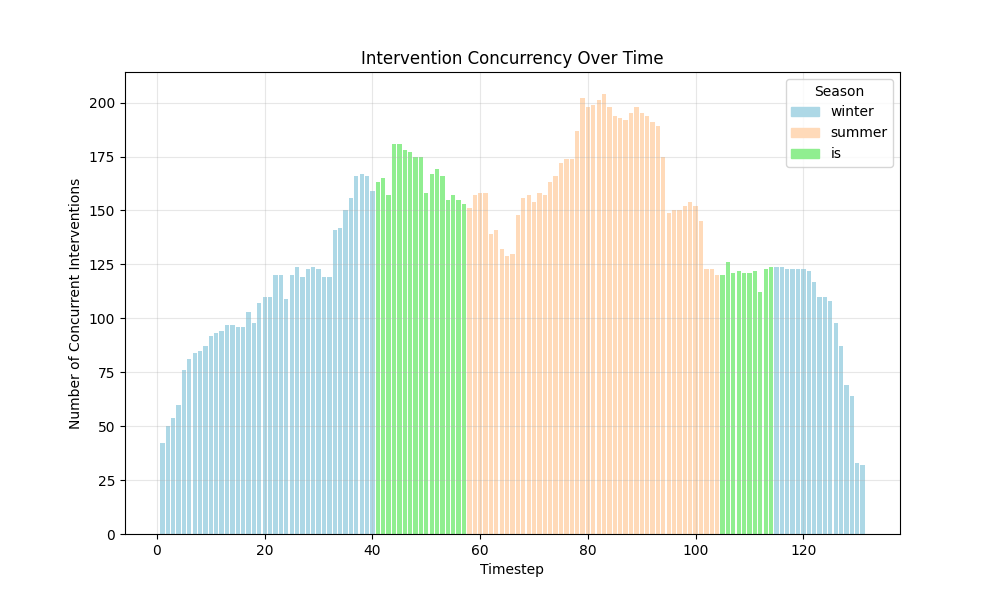
\includegraphics[width=\textwidth]{ch3/figures/Concurrency.png}
    \caption{Concurrent interventions over time for an example solution, showing the number of interventions being executed simultaneously at each time period. Colors are used to differentiate seasons.}
    \label{fig:concurrency}
\end{figure}



% \paragraph{Highest Risk:} This attribute measures the average worst-case risk across all interventions, where for each intervention we consider its maximum risk over all time periods and scenarios. Formally, we have:

% \[\operatorname{worst}^{(i,\tau)} \coleq \max_{t=1,\dots,d_{i,\tau}} \max_{s\in S} \mathrm{risk}_{s,t}^{(i,\tau)} \quad \text{where} \quad \text{highest\_risk} \coleq \frac{1}{|\mathcal{I}|}\sum_{i\in\mathcal{I}} \operatorname{worst}^{(i,\tau_i)}\]



\paragraph{Seasonality:} These are 3 attributes that indicate the proportion of total interventions active in each season (Winter, Summer, or Interseason). Note that the proportions sum to more than 1 since interventions can span multiple seasons.

\subsection{Fuzzy Attributes}
In this section, 4 categories of attributes are defined using two concepts from fuzzy logic. Our approach will be to define these properties for each intervention.

First we define a fuzzy linguistic variable for each attribute. In the case of distances (between interventions and between parks and interventions), we will assign its values using fuzzy numbers, in specific trapezoidal and triangular fuzzy numbers (see figure \ref{fig:fuzzy_distance}). On the other hand, memberships to degrees of size and degrees of risk will be assigned via fuzzy cmeans, where each intervention may have multiple non-zero membership degrees to different clusters, their centroids can be seen in table \ref{tab:fuzzy_centroids}.

\begin{table}[!ht]
    \centering
    \begin{tabular}{lcc}
    \hline
    \textbf{Cluster Type} & \textbf{Size Centroids} & \textbf{Risk Centroids} \\
    \hline
    Small/Low & 389.36 & 972.16 \\
    Mid-small/Mid-low & 4,616.21 & 987.10 \\
    Medium/Mid & 8,304.83 & 997.60 \\
    Mid-large/Mid-high & 12,653.61 & 1,009.31 \\
    Large/High & 23,279.25 & 1,024.11 \\
    \hline
    \end{tabular}
    \caption{Fuzzy cluster centroids for intervention size and risk levels.}
    \label{tab:fuzzy_centroids}
    \end{table}
    
    
    \begin{figure}[!ht]
    \centering
    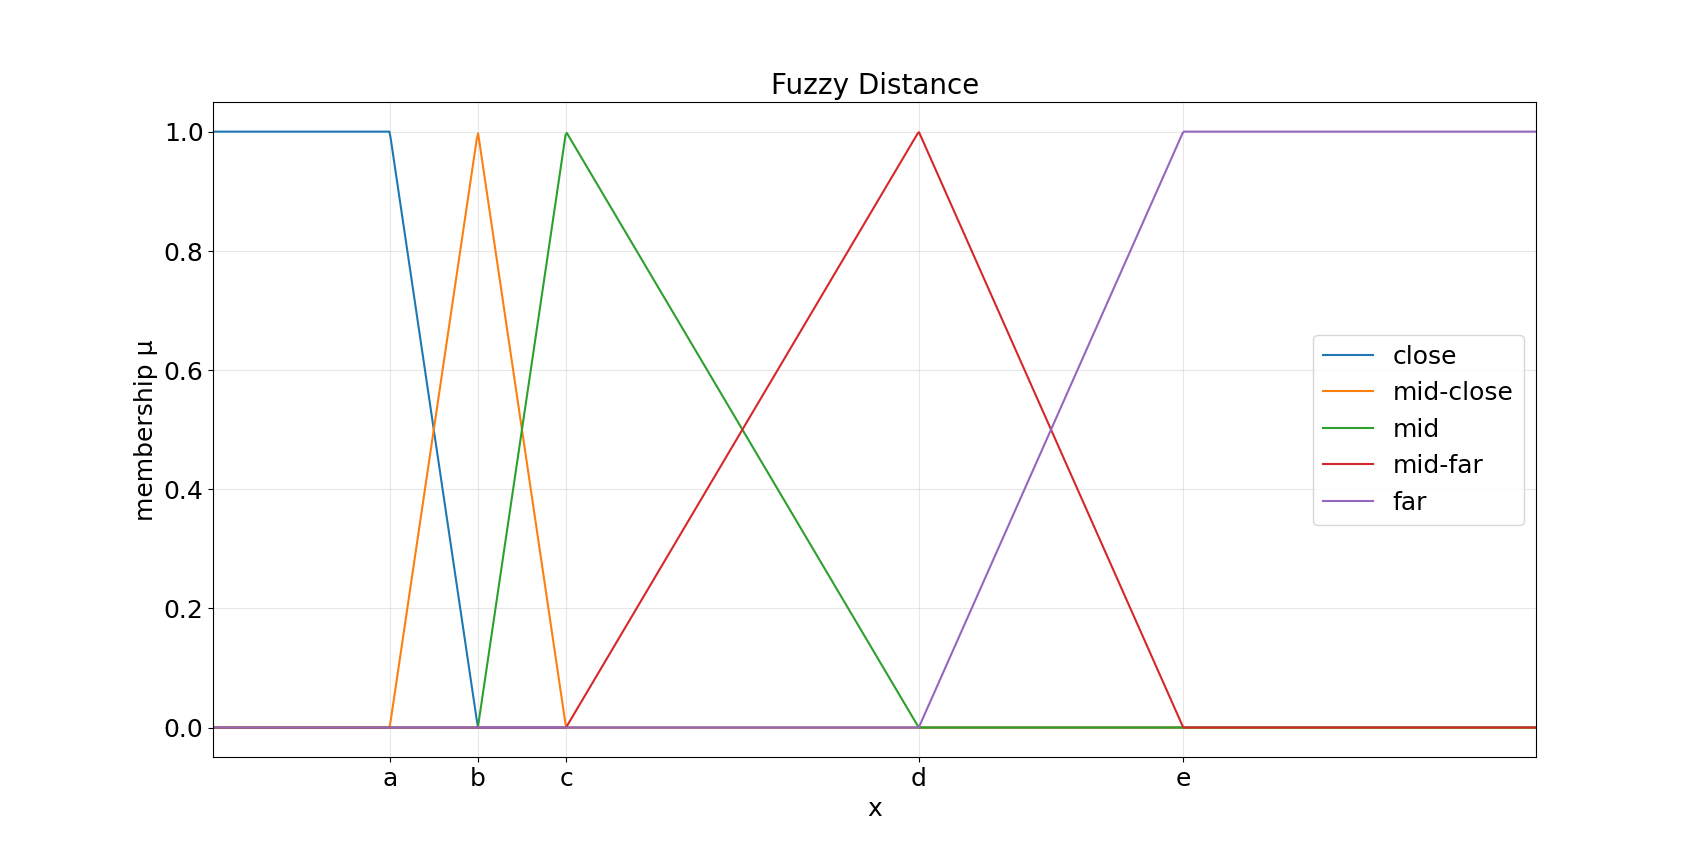
\includegraphics[width=\linewidth]{ch3/figures/Fuzzy distance.png}
    \caption{Fuzzy distance linguistic variable with close, mid-close, mid, mid-far and far membership functions.}
    \label{fig:fuzzy_distance}
    \end{figure}

In order to go from the membership values of interventions to membership values of a particular solution, we will leverage the distribution of daily masses of memberships over the planning horizon.

The idea is the following:

In the case of the distance matrix of distances intervention to intervention. We start by applying the fuzzy variable to the crisp distance matrix. This is a mapping from a real valued distance to 5 membership values, which can be represented with 5 matrices, one for each fuzzy distance (intervention to intervention) set. This are 5 fuzzy sets over the pairs of interventions. Afterwards, to compute the daily mass of each of those 5 fuzzy sets, we are going to take the cardinality of the each of those 5 fuzzy sets restricted to the unique pairs of active interventions in a day. Do this for each day in the time horizon. After that, we have a unique mass value for each day (see figure \ref{fig:fuzzy_att_concurrency}). 

In the case of the distance matrix from interventions (rows) to parks (colums). The approach is similar, we apply a different fuzzy distance variable and get 5 matrices. But in this case, since columns represent parks instead of interventions, we aggregate row wise each matrix using a t-conorm which converts each of the five matrices into a vector which corresponds to a five closeness to park value per intervention. Which are 5 closeness to park membership vectors (a fuzzy set over the set of interventions). Then the approach to generate the daily masses is analogous to the previous case. We take the fuzzy subset corresponding to the active interventions in any given day and add their memberships (cardinal of that fuzzy subset).

Regarding the risk and size, we have a mean size and a mean risk for each intervention (a vector). This is then fuzzy clustered into 5 clusters, therefore converting each vector of mean values into 5 vectors of memberships. Then the daily masses are computed analogously to the vectors from the distances to parks.

 

\begin{figure}[!ht]
    \begin{adjustwidth}{-1.6cm}{-1.6cm}
    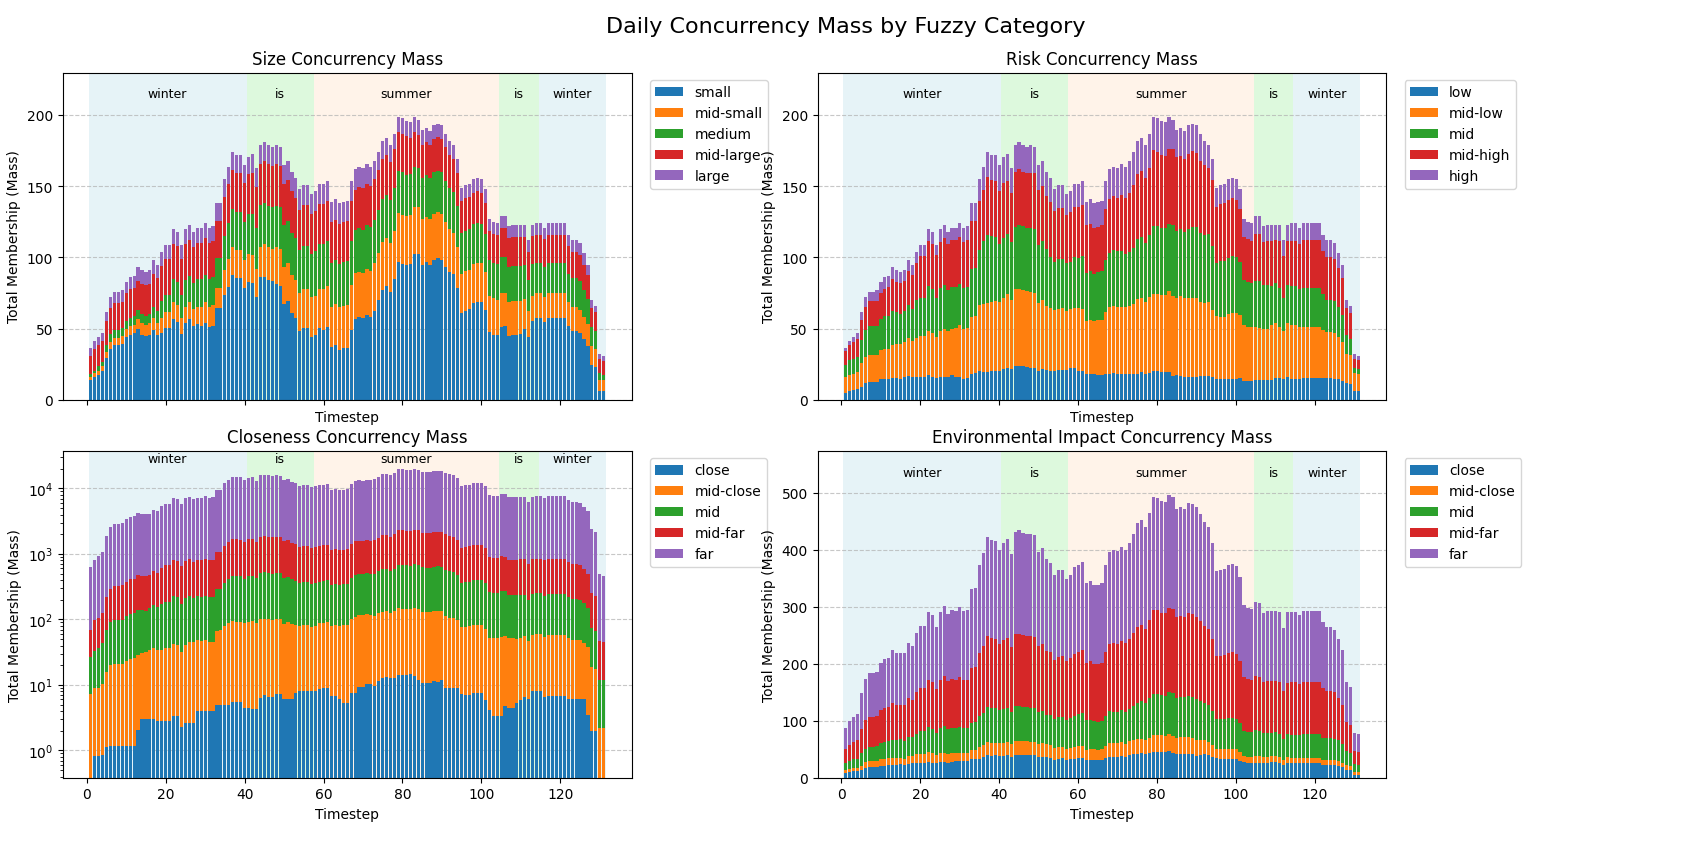
\includegraphics[width=1.07\linewidth]{ch3/figures/Fuzzy_att_concurrency.png}
    \end{adjustwidth}
    \caption{Distribution of daily masses of membership for an example solution throughout the planning horizon.}
    \label{fig:fuzzy_att_concurrency}
\end{figure}



\paragraph{Closeness Concurrency:} This attribute quantifies the degree to which interventions that are spatially "close" occur simultaneously. At each timestep \(t\), let \(\mathcal{I}(t)\) be the set of interventions active. For every unique pair \(\{i,j\}\) in \(\mathcal{I}(t)\), we...


\paragraph{Environmental Impact Concurrency:} This score quantifies the level of simultaneous interventions with different degrees of environmental impact over the planning horizon. At each timestep \(t\), let \(\mathcal{I}(t)\) denote the set of active interventions. 

\paragraph{Size Concurrency:} This attribute quantifies the degree of overlap among interventions with significant workload sizes. 

First, we compute the \textbf{mean intervention size}: For each intervention \(i\), we consider all possible start times \(\tau\). For each start time \(\tau\), the total workload is used to compute the mean intervention size for intervention \(i\):

\[
    \text{mean\_size}_i \coleq \frac{1}{|\mathcal{T}_i|} \sum_{\tau\in \mathcal{T}_i} \text{size}_{i,\tau},
    \qquad \text{with }\,
    \text{size}_{i,\tau} \coleq \left(\sum_{c \in C} \sum_{t=1}^{T} r_{c,t}(i,\tau)\right) \times d_{i,\tau}, \,\, \mathcal{T}_i = \{ \tau \mid \text{size}_{i,\tau} > 0 \}
\]

where \(C\) is the set of resources, \(r_{c,t}(i,\tau)\) is the consumption of resource \(c\) at time \(t\) when intervention \(i\) starts at \(\tau\), and \(d_{i,\tau}\) is the duration. Only start times with non-zero \(\text{size}_{i,\tau}\) are considered. 


Then, interventions are clustered into \texttt{small}, \texttt{mid-small},\texttt{mid}, \texttt{mid-large} and \texttt{large} groups using fuzzy cmeans on their mean intervention sizes. At each timestep \(t\), let \(\mathcal{I}(t)\) denote the set of active interventions. 

\paragraph{Risk Concurrency:} Analogous to size concurrency, risk concurrency quantifies the degree of overlap among interventions with elevated risk levels. In this case, each intervention \(i\in I\) has a risk value which is the average of its nonzero risk values $r_t^{(i)}$ (see Assumption 1) across all start times. Then, interventions are clustered via fuzzy cmeans into... The score is completely identical to the one from size concurrency.




Finally, each daily mass distribution (we have 5 linguistic values $\times$ 4 linguistic variables = 20 mass distributions). 

Since the total mass is the same for all the solutions (they all have to schedule the exact same interventions) and what varies is how that mass is distributed across the time horizon. We are going to consider that what would be best is to have those masses uniformly distributed and what would be worse is to have a peak day where all the dangerous, risky, huge and concentered in one place interventions, take place. With this intention we are going to normalize each distribution by their total mass (the shape of the distribution remains the same) and then take the minus entropy of that distribution.

Notice that here, we do not have any probabilities and entropy only serves as a measure of how uniformity. No information or probabilistic interpretation would make sense in this case.

In their foundational work, Cover and Thomas define the entropy $H(X)$ of a discrete random variable $X$ as a measure of uncertainty or randomness associated with the possible outcomes \cite[Section 2.1]{Entropy}. The entropy is calculated by the following formula:
\[
H(X) = - \sum_x p(x)\, \log p(x)
\]
where $p(x)$ denotes the probability of outcome $x$.

According to Cover and Thomas \cite[p.~14]{Entropy}, entropy is minimized when the distribution is deterministic, meaning that a single outcome has probability one and all others have probability zero. In this case, $H(X)=0$, reflecting the absence of uncertainty. Conversely, entropy is maximized by the uniform distribution. Specifically, for a variable $X$ with $|X|$ possible outcomes, the entropy satisfies the inequality
\[
H(X) \leq \log |X| 
\]
with equality if and only if $X$ is uniformly distributed \cite[Theorem 2.6.4, p.~27]{Entropy}. Therefore, a uniform distribution corresponds to maximum entropy, while a deterministic distribution yields the minimum possible entropy.




\clearpage
\newgeometry{bottom=0.6cm}
\begin{sidewaystable}[!ht]
\thispagestyle{empty}
\centering
\scriptsize
\setlength\tabcolsep{3pt}
\renewcommand{\arraystretch}{1.5}
\resizebox{1.12\textheight}{!}{

\begin{tabular}{|l|c|ccccc|ccccc|ccccc|ccccc|ccc|}
\hline

\multirow{2}{*}{\rule{0pt}{2.3ex}\textbf{Solutions}} &
\multirow{2}{*}{\rule{0pt}{2.3ex}\shortstack{\textbf{Highest}\\\textbf{Concurrency}}} &
\multicolumn{5}{c|}{\textbf{Size Concurrency}} &
\multicolumn{5}{c|}{\textbf{Risk Concurrency}} &
\multicolumn{5}{c|}{\textbf{Closeness Concurrency}} &
\multicolumn{5}{c|}{\textbf{Environmental-Impact Concurrency}} &
\multicolumn{3}{c|}{\textbf{Seasonality}} \\[2pt]
& & \cellcolor{SizeBase!10}small & \cellcolor{SizeBase!20}mid-small & \cellcolor{SizeBase!30}mid & \cellcolor{SizeBase!40}mid-large & \cellcolor{SizeBase!50}large & \cellcolor{RiskBase!10}low & \cellcolor{RiskBase!20}mid-low & \cellcolor{RiskBase!30}mid & \cellcolor{RiskBase!40}mid-high & \cellcolor{RiskBase!50}high & \cellcolor{CloseBase!10}close & \cellcolor{CloseBase!20}mid-close & \cellcolor{CloseBase!30}mid & \cellcolor{CloseBase!40}mid-far & \cellcolor{CloseBase!50}far & \cellcolor{EnvBase!10}low & \cellcolor{EnvBase!20}mid-low & \cellcolor{EnvBase!30}mid & \cellcolor{EnvBase!40}mid-high & \cellcolor{EnvBase!50}high & \cellcolor{Winter}Winter & \cellcolor{Summer}Summer & \cellcolor{Inter}Inter-season \\
\hline
T1\_D180\_S33 & 0.392 & \cellcolor{SizeBase!10}0.987 & \cellcolor{SizeBase!20}0.982 & \cellcolor{SizeBase!30}0.982 & \cellcolor{SizeBase!40}0.996 & \cellcolor{SizeBase!50}0.993 & \cellcolor{RiskBase!10}0.994 & \cellcolor{RiskBase!20}0.990 & \cellcolor{RiskBase!30}0.990 & \cellcolor{RiskBase!40}0.990 & \cellcolor{RiskBase!50}0.984 & \cellcolor{CloseBase!10}0.971 & \cellcolor{CloseBase!20}0.972 & \cellcolor{CloseBase!30}0.970 & \cellcolor{CloseBase!40}0.972 & \cellcolor{CloseBase!50}0.972 & \cellcolor{EnvBase!10}0.990 & \cellcolor{EnvBase!20}0.986 & \cellcolor{EnvBase!30}0.990 & \cellcolor{EnvBase!40}0.991 & \cellcolor{EnvBase!50}0.991 & \cellcolor{Winter}0.618 & \cellcolor{Summer}0.622 & \cellcolor{Inter}0.607 \\
T1\_D180\_S42 & 0.390 & \cellcolor{SizeBase!10}0.987 & \cellcolor{SizeBase!20}0.983 & \cellcolor{SizeBase!30}0.984 & \cellcolor{SizeBase!40}0.996 & \cellcolor{SizeBase!50}0.993 & \cellcolor{RiskBase!10}0.995 & \cellcolor{RiskBase!20}0.991 & \cellcolor{RiskBase!30}0.990 & \cellcolor{RiskBase!40}0.989 & \cellcolor{RiskBase!50}0.983 & \cellcolor{CloseBase!10}0.967 & \cellcolor{CloseBase!20}0.973 & \cellcolor{CloseBase!30}0.971 & \cellcolor{CloseBase!40}0.972 & \cellcolor{CloseBase!50}0.972 & \cellcolor{EnvBase!10}0.990 & \cellcolor{EnvBase!20}0.985 & \cellcolor{EnvBase!30}0.990 & \cellcolor{EnvBase!40}0.991 & \cellcolor{EnvBase!50}0.991 & \cellcolor{Winter}0.624 & \cellcolor{Summer}0.622 & \cellcolor{Inter}0.601 \\
T1\_D180\_S73 & 0.386 & \cellcolor{SizeBase!10}0.986 & \cellcolor{SizeBase!20}0.982 & \cellcolor{SizeBase!30}0.985 & \cellcolor{SizeBase!40}0.996 & \cellcolor{SizeBase!50}0.992 & \cellcolor{RiskBase!10}0.993 & \cellcolor{RiskBase!20}0.990 & \cellcolor{RiskBase!30}0.990 & \cellcolor{RiskBase!40}0.990 & \cellcolor{RiskBase!50}0.983 & \cellcolor{CloseBase!10}0.975 & \cellcolor{CloseBase!20}0.973 & \cellcolor{CloseBase!30}0.970 & \cellcolor{CloseBase!40}0.971 & \cellcolor{CloseBase!50}0.972 & \cellcolor{EnvBase!10}0.988 & \cellcolor{EnvBase!20}0.985 & \cellcolor{EnvBase!30}0.989 & \cellcolor{EnvBase!40}0.990 & \cellcolor{EnvBase!50}0.991 & \cellcolor{Winter}0.610 & \cellcolor{Summer}0.628 & \cellcolor{Inter}0.597 \\
T1\_D300\_S33 & 0.378 & \cellcolor{SizeBase!10}0.986 & \cellcolor{SizeBase!20}0.976 & \cellcolor{SizeBase!30}0.980 & \cellcolor{SizeBase!40}0.996 & \cellcolor{SizeBase!50}0.993 & \cellcolor{RiskBase!10}0.994 & \cellcolor{RiskBase!20}0.990 & \cellcolor{RiskBase!30}0.988 & \cellcolor{RiskBase!40}0.989 & \cellcolor{RiskBase!50}0.983 & \cellcolor{CloseBase!10}0.970 & \cellcolor{CloseBase!20}0.972 & \cellcolor{CloseBase!30}0.969 & \cellcolor{CloseBase!40}0.969 & \cellcolor{CloseBase!50}0.970 & \cellcolor{EnvBase!10}0.990 & \cellcolor{EnvBase!20}0.982 & \cellcolor{EnvBase!30}0.989 & \cellcolor{EnvBase!40}0.989 & \cellcolor{EnvBase!50}0.990 & \cellcolor{Winter}0.620 & \cellcolor{Summer}0.622 & \cellcolor{Inter}0.622 \\
T1\_D300\_S42 & 0.382 & \cellcolor{SizeBase!10}0.986 & \cellcolor{SizeBase!20}0.977 & \cellcolor{SizeBase!30}0.980 & \cellcolor{SizeBase!40}0.996 & \cellcolor{SizeBase!50}0.993 & \cellcolor{RiskBase!10}0.994 & \cellcolor{RiskBase!20}0.989 & \cellcolor{RiskBase!30}0.988 & \cellcolor{RiskBase!40}0.990 & \cellcolor{RiskBase!50}0.983 & \cellcolor{CloseBase!10}0.968 & \cellcolor{CloseBase!20}0.970 & \cellcolor{CloseBase!30}0.969 & \cellcolor{CloseBase!40}0.969 & \cellcolor{CloseBase!50}0.971 & \cellcolor{EnvBase!10}0.990 & \cellcolor{EnvBase!20}0.983 & \cellcolor{EnvBase!30}0.990 & \cellcolor{EnvBase!40}0.989 & \cellcolor{EnvBase!50}0.990 & \cellcolor{Winter}0.614 & \cellcolor{Summer}0.626 & \cellcolor{Inter}0.616 \\
T1\_D300\_S73 & 0.384 & \cellcolor{SizeBase!10}0.985 & \cellcolor{SizeBase!20}0.977 & \cellcolor{SizeBase!30}0.987 & \cellcolor{SizeBase!40}0.996 & \cellcolor{SizeBase!50}0.993 & \cellcolor{RiskBase!10}0.993 & \cellcolor{RiskBase!20}0.991 & \cellcolor{RiskBase!30}0.988 & \cellcolor{RiskBase!40}0.991 & \cellcolor{RiskBase!50}0.980 & \cellcolor{CloseBase!10}0.965 & \cellcolor{CloseBase!20}0.975 & \cellcolor{CloseBase!30}0.969 & \cellcolor{CloseBase!40}0.970 & \cellcolor{CloseBase!50}0.970 & \cellcolor{EnvBase!10}0.989 & \cellcolor{EnvBase!20}0.986 & \cellcolor{EnvBase!30}0.990 & \cellcolor{EnvBase!40}0.990 & \cellcolor{EnvBase!50}0.990 & \cellcolor{Winter}0.610 & \cellcolor{Summer}0.630 & \cellcolor{Inter}0.597 \\
T1\_D500\_S33 & 0.401 & \cellcolor{SizeBase!10}0.985 & \cellcolor{SizeBase!20}0.973 & \cellcolor{SizeBase!30}0.983 & \cellcolor{SizeBase!40}0.996 & \cellcolor{SizeBase!50}0.993 & \cellcolor{RiskBase!10}0.996 & \cellcolor{RiskBase!20}0.986 & \cellcolor{RiskBase!30}0.989 & \cellcolor{RiskBase!40}0.989 & \cellcolor{RiskBase!50}0.984 & \cellcolor{CloseBase!10}0.968 & \cellcolor{CloseBase!20}0.971 & \cellcolor{CloseBase!30}0.966 & \cellcolor{CloseBase!40}0.968 & \cellcolor{CloseBase!50}0.969 & \cellcolor{EnvBase!10}0.990 & \cellcolor{EnvBase!20}0.982 & \cellcolor{EnvBase!30}0.990 & \cellcolor{EnvBase!40}0.989 & \cellcolor{EnvBase!50}0.990 & \cellcolor{Winter}0.610 & \cellcolor{Summer}0.633 & \cellcolor{Inter}0.597 \\
T1\_D500\_S42 & 0.399 & \cellcolor{SizeBase!10}0.985 & \cellcolor{SizeBase!20}0.972 & \cellcolor{SizeBase!30}0.983 & \cellcolor{SizeBase!40}0.996 & \cellcolor{SizeBase!50}0.993 & \cellcolor{RiskBase!10}0.995 & \cellcolor{RiskBase!20}0.987 & \cellcolor{RiskBase!30}0.988 & \cellcolor{RiskBase!40}0.989 & \cellcolor{RiskBase!50}0.984 & \cellcolor{CloseBase!10}0.968 & \cellcolor{CloseBase!20}0.972 & \cellcolor{CloseBase!30}0.967 & \cellcolor{CloseBase!40}0.967 & \cellcolor{CloseBase!50}0.968 & \cellcolor{EnvBase!10}0.989 & \cellcolor{EnvBase!20}0.984 & \cellcolor{EnvBase!30}0.991 & \cellcolor{EnvBase!40}0.989 & \cellcolor{EnvBase!50}0.989 & \cellcolor{Winter}0.608 & \cellcolor{Summer}0.633 & \cellcolor{Inter}0.597 \\
T1\_D500\_S73 & 0.395 & \cellcolor{SizeBase!10}0.986 & \cellcolor{SizeBase!20}0.972 & \cellcolor{SizeBase!30}0.983 & \cellcolor{SizeBase!40}0.996 & \cellcolor{SizeBase!50}0.993 & \cellcolor{RiskBase!10}0.994 & \cellcolor{RiskBase!20}0.987 & \cellcolor{RiskBase!30}0.988 & \cellcolor{RiskBase!40}0.989 & \cellcolor{RiskBase!50}0.983 & \cellcolor{CloseBase!10}0.965 & \cellcolor{CloseBase!20}0.971 & \cellcolor{CloseBase!30}0.966 & \cellcolor{CloseBase!40}0.968 & \cellcolor{CloseBase!50}0.969 & \cellcolor{EnvBase!10}0.990 & \cellcolor{EnvBase!20}0.984 & \cellcolor{EnvBase!30}0.991 & \cellcolor{EnvBase!40}0.989 & \cellcolor{EnvBase!50}0.990 & \cellcolor{Winter}0.608 & \cellcolor{Summer}0.633 & \cellcolor{Inter}0.603 \\
T1\_D700\_S33 & 0.403 & \cellcolor{SizeBase!10}0.985 & \cellcolor{SizeBase!20}0.974 & \cellcolor{SizeBase!30}0.984 & \cellcolor{SizeBase!40}0.996 & \cellcolor{SizeBase!50}0.992 & \cellcolor{RiskBase!10}0.996 & \cellcolor{RiskBase!20}0.987 & \cellcolor{RiskBase!30}0.989 & \cellcolor{RiskBase!40}0.989 & \cellcolor{RiskBase!50}0.983 & \cellcolor{CloseBase!10}0.968 & \cellcolor{CloseBase!20}0.971 & \cellcolor{CloseBase!30}0.966 & \cellcolor{CloseBase!40}0.968 & \cellcolor{CloseBase!50}0.969 & \cellcolor{EnvBase!10}0.990 & \cellcolor{EnvBase!20}0.985 & \cellcolor{EnvBase!30}0.990 & \cellcolor{EnvBase!40}0.989 & \cellcolor{EnvBase!50}0.990 & \cellcolor{Winter}0.610 & \cellcolor{Summer}0.630 & \cellcolor{Inter}0.607 \\
T1\_D700\_S42 & 0.393 & \cellcolor{SizeBase!10}0.985 & \cellcolor{SizeBase!20}0.974 & \cellcolor{SizeBase!30}0.984 & \cellcolor{SizeBase!40}0.996 & \cellcolor{SizeBase!50}0.992 & \cellcolor{RiskBase!10}0.996 & \cellcolor{RiskBase!20}0.987 & \cellcolor{RiskBase!30}0.988 & \cellcolor{RiskBase!40}0.989 & \cellcolor{RiskBase!50}0.983 & \cellcolor{CloseBase!10}0.971 & \cellcolor{CloseBase!20}0.972 & \cellcolor{CloseBase!30}0.967 & \cellcolor{CloseBase!40}0.968 & \cellcolor{CloseBase!50}0.969 & \cellcolor{EnvBase!10}0.989 & \cellcolor{EnvBase!20}0.984 & \cellcolor{EnvBase!30}0.991 & \cellcolor{EnvBase!40}0.989 & \cellcolor{EnvBase!50}0.990 & \cellcolor{Winter}0.610 & \cellcolor{Summer}0.631 & \cellcolor{Inter}0.595 \\
T1\_D700\_S73 & 0.390 & \cellcolor{SizeBase!10}0.985 & \cellcolor{SizeBase!20}0.973 & \cellcolor{SizeBase!30}0.984 & \cellcolor{SizeBase!40}0.996 & \cellcolor{SizeBase!50}0.992 & \cellcolor{RiskBase!10}0.995 & \cellcolor{RiskBase!20}0.987 & \cellcolor{RiskBase!30}0.989 & \cellcolor{RiskBase!40}0.989 & \cellcolor{RiskBase!50}0.985 & \cellcolor{CloseBase!10}0.969 & \cellcolor{CloseBase!20}0.971 & \cellcolor{CloseBase!30}0.967 & \cellcolor{CloseBase!40}0.968 & \cellcolor{CloseBase!50}0.969 & \cellcolor{EnvBase!10}0.990 & \cellcolor{EnvBase!20}0.985 & \cellcolor{EnvBase!30}0.991 & \cellcolor{EnvBase!40}0.989 & \cellcolor{EnvBase!50}0.990 & \cellcolor{Winter}0.610 & \cellcolor{Summer}0.630 & \cellcolor{Inter}0.608 \\
T1\_D900\_S33 & 0.388 & \cellcolor{SizeBase!10}0.983 & \cellcolor{SizeBase!20}0.976 & \cellcolor{SizeBase!30}0.984 & \cellcolor{SizeBase!40}0.996 & \cellcolor{SizeBase!50}0.993 & \cellcolor{RiskBase!10}0.995 & \cellcolor{RiskBase!20}0.986 & \cellcolor{RiskBase!30}0.987 & \cellcolor{RiskBase!40}0.989 & \cellcolor{RiskBase!50}0.986 & \cellcolor{CloseBase!10}0.965 & \cellcolor{CloseBase!20}0.971 & \cellcolor{CloseBase!30}0.966 & \cellcolor{CloseBase!40}0.967 & \cellcolor{CloseBase!50}0.968 & \cellcolor{EnvBase!10}0.989 & \cellcolor{EnvBase!20}0.982 & \cellcolor{EnvBase!30}0.990 & \cellcolor{EnvBase!40}0.988 & \cellcolor{EnvBase!50}0.989 & \cellcolor{Winter}0.601 & \cellcolor{Summer}0.641 & \cellcolor{Inter}0.605 \\
T1\_D900\_S42 & 0.395 & \cellcolor{SizeBase!10}0.985 & \cellcolor{SizeBase!20}0.973 & \cellcolor{SizeBase!30}0.985 & \cellcolor{SizeBase!40}0.996 & \cellcolor{SizeBase!50}0.992 & \cellcolor{RiskBase!10}0.996 & \cellcolor{RiskBase!20}0.986 & \cellcolor{RiskBase!30}0.988 & \cellcolor{RiskBase!40}0.989 & \cellcolor{RiskBase!50}0.984 & \cellcolor{CloseBase!10}0.961 & \cellcolor{CloseBase!20}0.971 & \cellcolor{CloseBase!30}0.966 & \cellcolor{CloseBase!40}0.967 & \cellcolor{CloseBase!50}0.968 & \cellcolor{EnvBase!10}0.990 & \cellcolor{EnvBase!20}0.983 & \cellcolor{EnvBase!30}0.990 & \cellcolor{EnvBase!40}0.989 & \cellcolor{EnvBase!50}0.990 & \cellcolor{Winter}0.607 & \cellcolor{Summer}0.633 & \cellcolor{Inter}0.608 \\
T1\_D900\_S73 & 0.395 & \cellcolor{SizeBase!10}0.985 & \cellcolor{SizeBase!20}0.975 & \cellcolor{SizeBase!30}0.984 & \cellcolor{SizeBase!40}0.996 & \cellcolor{SizeBase!50}0.993 & \cellcolor{RiskBase!10}0.995 & \cellcolor{RiskBase!20}0.986 & \cellcolor{RiskBase!30}0.990 & \cellcolor{RiskBase!40}0.990 & \cellcolor{RiskBase!50}0.985 & \cellcolor{CloseBase!10}0.969 & \cellcolor{CloseBase!20}0.973 & \cellcolor{CloseBase!30}0.967 & \cellcolor{CloseBase!40}0.968 & \cellcolor{CloseBase!50}0.969 & \cellcolor{EnvBase!10}0.989 & \cellcolor{EnvBase!20}0.985 & \cellcolor{EnvBase!30}0.991 & \cellcolor{EnvBase!40}0.989 & \cellcolor{EnvBase!50}0.990 & \cellcolor{Winter}0.603 & \cellcolor{Summer}0.635 & \cellcolor{Inter}0.595 \\
T3\_D180\_S33 & 0.401 & \cellcolor{SizeBase!10}0.985 & \cellcolor{SizeBase!20}0.972 & \cellcolor{SizeBase!30}0.985 & \cellcolor{SizeBase!40}0.996 & \cellcolor{SizeBase!50}0.991 & \cellcolor{RiskBase!10}0.994 & \cellcolor{RiskBase!20}0.985 & \cellcolor{RiskBase!30}0.989 & \cellcolor{RiskBase!40}0.990 & \cellcolor{RiskBase!50}0.983 & \cellcolor{CloseBase!10}0.962 & \cellcolor{CloseBase!20}0.971 & \cellcolor{CloseBase!30}0.967 & \cellcolor{CloseBase!40}0.967 & \cellcolor{CloseBase!50}0.969 & \cellcolor{EnvBase!10}0.990 & \cellcolor{EnvBase!20}0.983 & \cellcolor{EnvBase!30}0.989 & \cellcolor{EnvBase!40}0.989 & \cellcolor{EnvBase!50}0.990 & \cellcolor{Winter}0.605 & \cellcolor{Summer}0.637 & \cellcolor{Inter}0.605 \\
T3\_D180\_S42 & 0.393 & \cellcolor{SizeBase!10}0.985 & \cellcolor{SizeBase!20}0.976 & \cellcolor{SizeBase!30}0.984 & \cellcolor{SizeBase!40}0.996 & \cellcolor{SizeBase!50}0.993 & \cellcolor{RiskBase!10}0.994 & \cellcolor{RiskBase!20}0.987 & \cellcolor{RiskBase!30}0.989 & \cellcolor{RiskBase!40}0.991 & \cellcolor{RiskBase!50}0.983 & \cellcolor{CloseBase!10}0.963 & \cellcolor{CloseBase!20}0.970 & \cellcolor{CloseBase!30}0.968 & \cellcolor{CloseBase!40}0.969 & \cellcolor{CloseBase!50}0.970 & \cellcolor{EnvBase!10}0.991 & \cellcolor{EnvBase!20}0.982 & \cellcolor{EnvBase!30}0.990 & \cellcolor{EnvBase!40}0.989 & \cellcolor{EnvBase!50}0.990 & \cellcolor{Winter}0.608 & \cellcolor{Summer}0.631 & \cellcolor{Inter}0.595 \\
T3\_D180\_S73 & 0.405 & \cellcolor{SizeBase!10}0.984 & \cellcolor{SizeBase!20}0.976 & \cellcolor{SizeBase!30}0.985 & \cellcolor{SizeBase!40}0.996 & \cellcolor{SizeBase!50}0.993 & \cellcolor{RiskBase!10}0.994 & \cellcolor{RiskBase!20}0.987 & \cellcolor{RiskBase!30}0.989 & \cellcolor{RiskBase!40}0.990 & \cellcolor{RiskBase!50}0.982 & \cellcolor{CloseBase!10}0.963 & \cellcolor{CloseBase!20}0.972 & \cellcolor{CloseBase!30}0.967 & \cellcolor{CloseBase!40}0.968 & \cellcolor{CloseBase!50}0.969 & \cellcolor{EnvBase!10}0.990 & \cellcolor{EnvBase!20}0.984 & \cellcolor{EnvBase!30}0.990 & \cellcolor{EnvBase!40}0.989 & \cellcolor{EnvBase!50}0.990 & \cellcolor{Winter}0.599 & \cellcolor{Summer}0.635 & \cellcolor{Inter}0.597 \\
T3\_D300\_S33 & 0.392 & \cellcolor{SizeBase!10}0.984 & \cellcolor{SizeBase!20}0.976 & \cellcolor{SizeBase!30}0.985 & \cellcolor{SizeBase!40}0.996 & \cellcolor{SizeBase!50}0.993 & \cellcolor{RiskBase!10}0.995 & \cellcolor{RiskBase!20}0.986 & \cellcolor{RiskBase!30}0.988 & \cellcolor{RiskBase!40}0.989 & \cellcolor{RiskBase!50}0.986 & \cellcolor{CloseBase!10}0.968 & \cellcolor{CloseBase!20}0.972 & \cellcolor{CloseBase!30}0.968 & \cellcolor{CloseBase!40}0.968 & \cellcolor{CloseBase!50}0.969 & \cellcolor{EnvBase!10}0.991 & \cellcolor{EnvBase!20}0.981 & \cellcolor{EnvBase!30}0.989 & \cellcolor{EnvBase!40}0.989 & \cellcolor{EnvBase!50}0.990 & \cellcolor{Winter}0.624 & \cellcolor{Summer}0.618 & \cellcolor{Inter}0.616 \\
T3\_D300\_S42 & 0.395 & \cellcolor{SizeBase!10}0.985 & \cellcolor{SizeBase!20}0.975 & \cellcolor{SizeBase!30}0.986 & \cellcolor{SizeBase!40}0.996 & \cellcolor{SizeBase!50}0.993 & \cellcolor{RiskBase!10}0.993 & \cellcolor{RiskBase!20}0.988 & \cellcolor{RiskBase!30}0.990 & \cellcolor{RiskBase!40}0.990 & \cellcolor{RiskBase!50}0.983 & \cellcolor{CloseBase!10}0.966 & \cellcolor{CloseBase!20}0.973 & \cellcolor{CloseBase!30}0.968 & \cellcolor{CloseBase!40}0.968 & \cellcolor{CloseBase!50}0.970 & \cellcolor{EnvBase!10}0.990 & \cellcolor{EnvBase!20}0.983 & \cellcolor{EnvBase!30}0.990 & \cellcolor{EnvBase!40}0.989 & \cellcolor{EnvBase!50}0.990 & \cellcolor{Winter}0.597 & \cellcolor{Summer}0.639 & \cellcolor{Inter}0.610 \\
T3\_D300\_S73 & 0.401 & \cellcolor{SizeBase!10}0.985 & \cellcolor{SizeBase!20}0.972 & \cellcolor{SizeBase!30}0.985 & \cellcolor{SizeBase!40}0.996 & \cellcolor{SizeBase!50}0.993 & \cellcolor{RiskBase!10}0.993 & \cellcolor{RiskBase!20}0.987 & \cellcolor{RiskBase!30}0.989 & \cellcolor{RiskBase!40}0.990 & \cellcolor{RiskBase!50}0.983 & \cellcolor{CloseBase!10}0.959 & \cellcolor{CloseBase!20}0.970 & \cellcolor{CloseBase!30}0.969 & \cellcolor{CloseBase!40}0.969 & \cellcolor{CloseBase!50}0.969 & \cellcolor{EnvBase!10}0.989 & \cellcolor{EnvBase!20}0.983 & \cellcolor{EnvBase!30}0.990 & \cellcolor{EnvBase!40}0.989 & \cellcolor{EnvBase!50}0.990 & \cellcolor{Winter}0.608 & \cellcolor{Summer}0.628 & \cellcolor{Inter}0.599 \\
T3\_D500\_S33 & 0.399 & \cellcolor{SizeBase!10}0.984 & \cellcolor{SizeBase!20}0.977 & \cellcolor{SizeBase!30}0.986 & \cellcolor{SizeBase!40}0.996 & \cellcolor{SizeBase!50}0.994 & \cellcolor{RiskBase!10}0.995 & \cellcolor{RiskBase!20}0.988 & \cellcolor{RiskBase!30}0.989 & \cellcolor{RiskBase!40}0.990 & \cellcolor{RiskBase!50}0.982 & \cellcolor{CloseBase!10}0.965 & \cellcolor{CloseBase!20}0.974 & \cellcolor{CloseBase!30}0.967 & \cellcolor{CloseBase!40}0.968 & \cellcolor{CloseBase!50}0.970 & \cellcolor{EnvBase!10}0.992 & \cellcolor{EnvBase!20}0.982 & \cellcolor{EnvBase!30}0.989 & \cellcolor{EnvBase!40}0.989 & \cellcolor{EnvBase!50}0.990 & \cellcolor{Winter}0.605 & \cellcolor{Summer}0.639 & \cellcolor{Inter}0.601 \\
T3\_D500\_S42 & 0.395 & \cellcolor{SizeBase!10}0.985 & \cellcolor{SizeBase!20}0.974 & \cellcolor{SizeBase!30}0.986 & \cellcolor{SizeBase!40}0.996 & \cellcolor{SizeBase!50}0.994 & \cellcolor{RiskBase!10}0.994 & \cellcolor{RiskBase!20}0.987 & \cellcolor{RiskBase!30}0.989 & \cellcolor{RiskBase!40}0.991 & \cellcolor{RiskBase!50}0.983 & \cellcolor{CloseBase!10}0.961 & \cellcolor{CloseBase!20}0.973 & \cellcolor{CloseBase!30}0.969 & \cellcolor{CloseBase!40}0.969 & \cellcolor{CloseBase!50}0.970 & \cellcolor{EnvBase!10}0.992 & \cellcolor{EnvBase!20}0.982 & \cellcolor{EnvBase!30}0.989 & \cellcolor{EnvBase!40}0.989 & \cellcolor{EnvBase!50}0.990 & \cellcolor{Winter}0.603 & \cellcolor{Summer}0.639 & \cellcolor{Inter}0.612 \\
T3\_D500\_S73 & 0.405 & \cellcolor{SizeBase!10}0.985 & \cellcolor{SizeBase!20}0.974 & \cellcolor{SizeBase!30}0.984 & \cellcolor{SizeBase!40}0.996 & \cellcolor{SizeBase!50}0.993 & \cellcolor{RiskBase!10}0.993 & \cellcolor{RiskBase!20}0.987 & \cellcolor{RiskBase!30}0.989 & \cellcolor{RiskBase!40}0.989 & \cellcolor{RiskBase!50}0.984 & \cellcolor{CloseBase!10}0.963 & \cellcolor{CloseBase!20}0.972 & \cellcolor{CloseBase!30}0.967 & \cellcolor{CloseBase!40}0.968 & \cellcolor{CloseBase!50}0.969 & \cellcolor{EnvBase!10}0.990 & \cellcolor{EnvBase!20}0.983 & \cellcolor{EnvBase!30}0.990 & \cellcolor{EnvBase!40}0.988 & \cellcolor{EnvBase!50}0.990 & \cellcolor{Winter}0.607 & \cellcolor{Summer}0.633 & \cellcolor{Inter}0.599 \\
T3\_D700\_S33 & 0.415 & \cellcolor{SizeBase!10}0.984 & \cellcolor{SizeBase!20}0.971 & \cellcolor{SizeBase!30}0.984 & \cellcolor{SizeBase!40}0.996 & \cellcolor{SizeBase!50}0.993 & \cellcolor{RiskBase!10}0.994 & \cellcolor{RiskBase!20}0.986 & \cellcolor{RiskBase!30}0.990 & \cellcolor{RiskBase!40}0.990 & \cellcolor{RiskBase!50}0.983 & \cellcolor{CloseBase!10}0.966 & \cellcolor{CloseBase!20}0.968 & \cellcolor{CloseBase!30}0.965 & \cellcolor{CloseBase!40}0.966 & \cellcolor{CloseBase!50}0.968 & \cellcolor{EnvBase!10}0.990 & \cellcolor{EnvBase!20}0.980 & \cellcolor{EnvBase!30}0.989 & \cellcolor{EnvBase!40}0.989 & \cellcolor{EnvBase!50}0.990 & \cellcolor{Winter}0.605 & \cellcolor{Summer}0.637 & \cellcolor{Inter}0.583 \\
T3\_D700\_S42 & 0.395 & \cellcolor{SizeBase!10}0.986 & \cellcolor{SizeBase!20}0.976 & \cellcolor{SizeBase!30}0.986 & \cellcolor{SizeBase!40}0.996 & \cellcolor{SizeBase!50}0.994 & \cellcolor{RiskBase!10}0.993 & \cellcolor{RiskBase!20}0.987 & \cellcolor{RiskBase!30}0.990 & \cellcolor{RiskBase!40}0.991 & \cellcolor{RiskBase!50}0.984 & \cellcolor{CloseBase!10}0.966 & \cellcolor{CloseBase!20}0.973 & \cellcolor{CloseBase!30}0.968 & \cellcolor{CloseBase!40}0.968 & \cellcolor{CloseBase!50}0.970 & \cellcolor{EnvBase!10}0.992 & \cellcolor{EnvBase!20}0.982 & \cellcolor{EnvBase!30}0.990 & \cellcolor{EnvBase!40}0.989 & \cellcolor{EnvBase!50}0.990 & \cellcolor{Winter}0.605 & \cellcolor{Summer}0.633 & \cellcolor{Inter}0.607 \\
T3\_D700\_S73 & 0.401 & \cellcolor{SizeBase!10}0.986 & \cellcolor{SizeBase!20}0.972 & \cellcolor{SizeBase!30}0.983 & \cellcolor{SizeBase!40}0.996 & \cellcolor{SizeBase!50}0.994 & \cellcolor{RiskBase!10}0.996 & \cellcolor{RiskBase!20}0.985 & \cellcolor{RiskBase!30}0.989 & \cellcolor{RiskBase!40}0.990 & \cellcolor{RiskBase!50}0.983 & \cellcolor{CloseBase!10}0.963 & \cellcolor{CloseBase!20}0.970 & \cellcolor{CloseBase!30}0.967 & \cellcolor{CloseBase!40}0.968 & \cellcolor{CloseBase!50}0.969 & \cellcolor{EnvBase!10}0.991 & \cellcolor{EnvBase!20}0.979 & \cellcolor{EnvBase!30}0.989 & \cellcolor{EnvBase!40}0.989 & \cellcolor{EnvBase!50}0.990 & \cellcolor{Winter}0.608 & \cellcolor{Summer}0.630 & \cellcolor{Inter}0.612 \\
T3\_D900\_S33 & 0.403 & \cellcolor{SizeBase!10}0.985 & \cellcolor{SizeBase!20}0.971 & \cellcolor{SizeBase!30}0.984 & \cellcolor{SizeBase!40}0.996 & \cellcolor{SizeBase!50}0.993 & \cellcolor{RiskBase!10}0.995 & \cellcolor{RiskBase!20}0.986 & \cellcolor{RiskBase!30}0.988 & \cellcolor{RiskBase!40}0.992 & \cellcolor{RiskBase!50}0.984 & \cellcolor{CloseBase!10}0.959 & \cellcolor{CloseBase!20}0.973 & \cellcolor{CloseBase!30}0.968 & \cellcolor{CloseBase!40}0.968 & \cellcolor{CloseBase!50}0.970 & \cellcolor{EnvBase!10}0.991 & \cellcolor{EnvBase!20}0.982 & \cellcolor{EnvBase!30}0.989 & \cellcolor{EnvBase!40}0.989 & \cellcolor{EnvBase!50}0.990 & \cellcolor{Winter}0.603 & \cellcolor{Summer}0.641 & \cellcolor{Inter}0.595 \\
T3\_D900\_S42 & 0.393 & \cellcolor{SizeBase!10}0.985 & \cellcolor{SizeBase!20}0.976 & \cellcolor{SizeBase!30}0.986 & \cellcolor{SizeBase!40}0.996 & \cellcolor{SizeBase!50}0.993 & \cellcolor{RiskBase!10}0.993 & \cellcolor{RiskBase!20}0.987 & \cellcolor{RiskBase!30}0.990 & \cellcolor{RiskBase!40}0.990 & \cellcolor{RiskBase!50}0.984 & \cellcolor{CloseBase!10}0.965 & \cellcolor{CloseBase!20}0.973 & \cellcolor{CloseBase!30}0.968 & \cellcolor{CloseBase!40}0.969 & \cellcolor{CloseBase!50}0.970 & \cellcolor{EnvBase!10}0.990 & \cellcolor{EnvBase!20}0.983 & \cellcolor{EnvBase!30}0.990 & \cellcolor{EnvBase!40}0.989 & \cellcolor{EnvBase!50}0.990 & \cellcolor{Winter}0.605 & \cellcolor{Summer}0.633 & \cellcolor{Inter}0.608 \\
T3\_D900\_S73 & 0.405 & \cellcolor{SizeBase!10}0.984 & \cellcolor{SizeBase!20}0.974 & \cellcolor{SizeBase!30}0.984 & \cellcolor{SizeBase!40}0.996 & \cellcolor{SizeBase!50}0.993 & \cellcolor{RiskBase!10}0.995 & \cellcolor{RiskBase!20}0.987 & \cellcolor{RiskBase!30}0.988 & \cellcolor{RiskBase!40}0.988 & \cellcolor{RiskBase!50}0.986 & \cellcolor{CloseBase!10}0.968 & \cellcolor{CloseBase!20}0.971 & \cellcolor{CloseBase!30}0.966 & \cellcolor{CloseBase!40}0.967 & \cellcolor{CloseBase!50}0.968 & \cellcolor{EnvBase!10}0.990 & \cellcolor{EnvBase!20}0.981 & \cellcolor{EnvBase!30}0.989 & \cellcolor{EnvBase!40}0.989 & \cellcolor{EnvBase!50}0.990 & \cellcolor{Winter}0.601 & \cellcolor{Summer}0.641 & \cellcolor{Inter}0.591 \\
T5\_D300\_S33 & 0.401 & \cellcolor{SizeBase!10}0.984 & \cellcolor{SizeBase!20}0.977 & \cellcolor{SizeBase!30}0.985 & \cellcolor{SizeBase!40}0.996 & \cellcolor{SizeBase!50}0.993 & \cellcolor{RiskBase!10}0.994 & \cellcolor{RiskBase!20}0.987 & \cellcolor{RiskBase!30}0.989 & \cellcolor{RiskBase!40}0.990 & \cellcolor{RiskBase!50}0.982 & \cellcolor{CloseBase!10}0.965 & \cellcolor{CloseBase!20}0.973 & \cellcolor{CloseBase!30}0.967 & \cellcolor{CloseBase!40}0.967 & \cellcolor{CloseBase!50}0.969 & \cellcolor{EnvBase!10}0.991 & \cellcolor{EnvBase!20}0.979 & \cellcolor{EnvBase!30}0.989 & \cellcolor{EnvBase!40}0.989 & \cellcolor{EnvBase!50}0.990 & \cellcolor{Winter}0.608 & \cellcolor{Summer}0.631 & \cellcolor{Inter}0.601 \\
\hline
\end{tabular}
}
\label{tab:dm_matrix}
\begin{adjustwidth}{2cm}{1.9cm}
\caption{Decision-making matrix containing broad categories of Size, Risk, Closure, and Environment. Each broad category is subdivided into 5 fuzzy attributes. Highest concurrency and seasonality (divided into Winter, Summer and Interseason) are crisp attributes. Teams are labeled as T1, T3 and T5 denoting the first, third and fifth ranked teams in the competition. For example, solution T1\_D180\_S33 represents Team 1 (competition winner), whose algorithm ran for 180 seconds with random seed 33.}
\end{adjustwidth}
\end{sidewaystable}
\restoregeometry
\section{Aggregation}
Given the decision matrix constructed in the previous section, the subsequent challenge is to aggregate this information into a single, comprehensive score to rank the alternatives. A flat aggregation, where a single operator like OWA is applied to all criteria simultaneously, would fail to capture the inherent hierarchical relationships and non-compensatory nature of the criteria. 
For instance, low risk concurrency should not compensate for high risk one. 
To address this, we adopt a two-level aggregation strategy, with a lexicographic model operating within distinct conceptual blocks and a separate fusion model operating across them, inspired by the framework proposed by Yager \cite{LOOWA}.\\

The first level of aggregation addresses the four blocks of fuzzy attributes: Size, Risk, Closeness, and Environmental Impact. Due to the problem's logic, the criteria within each block are organized according to a strict lexicographic ordering. For example, for the "Size" concept, the preference is for larger maintenance tasks to be spreaded uniformly, leading to the priority order: \texttt{Size\_large} $>$ \texttt{Size\_mid-large} $>$ \texttt{Size\_medium}, and so on. 
To model this, we employ the Lexicographic Ordinal OWA (LOOWA) operator. 
The intuition behind LOOWA is that a lower priority criterion can never compensate for a higher priority one. It can only confirm or decrease the score established by its superiors, making the block score effectively the highest performance level that can be guaranteed without violating any higher priority requirements.

Following the formulation from Yager's paper, for each alternative $x$, we first define $C_j(x)$ as the satisfaction (score from the matrix) of the $j$-th priority criterion ($j=1$ being most important). We then construct an adaptive importance gate $T_j(x)$ for each criterion:
\begin{equation}
T_1(x) = 1.0, \quad T_j(x) = \min_{k<j} C_k(x) \quad \text{for } j>1
\end{equation}

The final aggregated score for the block, $S(x)$, is calculated by taking the maximum of the satisfaction scores after each is capped by its corresponding gate:
\begin{equation}
S(x) = \max_{j=1...5} \left\{ \min \left( C_j(x), T_j(x) \right) \right\}
\end{equation}

Since $T_j(x) \leq C_1(x)$ for all $j>1$, the score $S(x)$ reduces to $C_1(x)$ whenever any lower priority criterion matches or exceeds the highest priority score. This ensures that lower priority attributes cannot raise the score. They only affect it when they fall below their predecessors, thereby lowering $S(x)$. While Yager originally developed LOOWA for ordinal evaluations, our implementation applies it to $[0,1]$ fuzzy membership degrees, where the join/meet operations naturally become max/min operations on real numbers.
This process is repeated for each of the four fuzzy blocks and for every alternative, transforming the 20 fuzzy attributes into four robust concept scores. The crisp attributes are handled separately: ``Highest Concurrency'' is a single value passed directly to the next stage, while the ``Seasonality'' attributes, which represent a trade-off rather than a hierarchy, are combined. Our implementation offers flexibility here, allowing for either a conventional weighted average or an OWA aggregation, depending on the decision-maker's preference. %<-- Change: Added detail about seasonality flexibility.
\\

The second level of aggregation fuses the resulting vector of six scores: (Concurrency, Size, Risk, Environmental Impact, Closeness, and Seasonality). At this stage, a key consideration is that providing precise, justifiable importance weights between these high-level concepts (e.g., is risk 1.5 times more important than environmental impact?) is often difficult and subjective. Therefore, an approach that is driven by the decision-maker's general attitude is more appropriate. We use the standard Ordered Weighted Averaging (OWA) operator for this purpose. OWA aggregates the concept scores based purely on their sorted values (in descending order), allowing the model to reflect optimism or pessimism. This behavior is controlled by the \textit{orness} parameter, $\alpha \in [0, 1]$. An orness of $\alpha=1$ (the maximum operator) reflects an optimistic attitude that judges a schedule by its strongest aspect, while $\alpha=0$ (the minimum operator) reflects a pessimistic, risk-averse stance that focuses on the weakest link. A neutral attitude (arithmetic mean) is achieved with $\alpha=0.5$.\\

%<-- Change: This entire paragraph is new, explaining the weight generation.
Therefore, OWA weights are generated systematically from the chosen $\alpha$ value using Yager's power-quantifier method instead of setting them manually. This method defines a basic unit monotone increasing quantifier $Q(r) = r^a$, where the exponent $a$ is derived from the desired orness:
\begin{equation}
a = \frac{2}{\alpha} - 2, \quad \text{for } \alpha \in (0, 1)
\end{equation}
The individual weights $w_i$ for an aggregation of $n$ items are then calculated as $w_i = Q(i/n) - Q((i-1)/n)$. This ensures that the set of weights is properly normalized and precisely reflects the decision-maker's specified attitude without requiring them to define each weight individually.
\\

In summary, our two-level model approach rests on two ideas: first, the predefined lexicographic ordering within each fuzzy block, and second, the attitudinal aggregation of the six main concepts. The practical implementation of this model in our analysis script requires the decision-maker to specify: %<-- Change: Minor rephrasing for flow.
\begin{romanenum}
    \item The \textbf{Seasonality preference}, specified either as a vector of weights (for a weighted average) or as an orness value (for an OWA aggregation).
    \item The outer-level \textbf{orness} $\alpha$, which defines their overall attitude, from pessimistic to optimistic, when balancing the performance across the six main concepts.
\end{romanenum}

\section{Results}
\label{sec:results}

The final stage of our analysis involves applying the two-level aggregation model to the decision matrix to rank the 29 alternative schedules. The model's flexibility allows a decision-maker to articulate their preferences through two sets of parameters: a preference for seasonality (3 weights) and an overall attitude towards risk, defined by the orness value $\alpha$. To showcase the model's behavior, we present the results across a spectrum of these parameters. Figure \ref{fig:results_plot} visualizes the outcomes for four distinct seasonal scenarios: a singular focus on each of the three seasons, and an equal weighting for all. 

The weight vectors for (Winter, Summer, Inter-season) used in these scenarios are (1.0, 0.0, 0.0) for "Winter focus", (0.0, 1.0, 0.0) for "Summer focus", (0.0, 0.0, 1.0) for "Inter-season", and (1/3, 1/3, 1/3) for "Equal weights"

\begin{figure}[h!]
    \centering
    \begin{adjustwidth}{-1.2cm}{-1.8cm}
    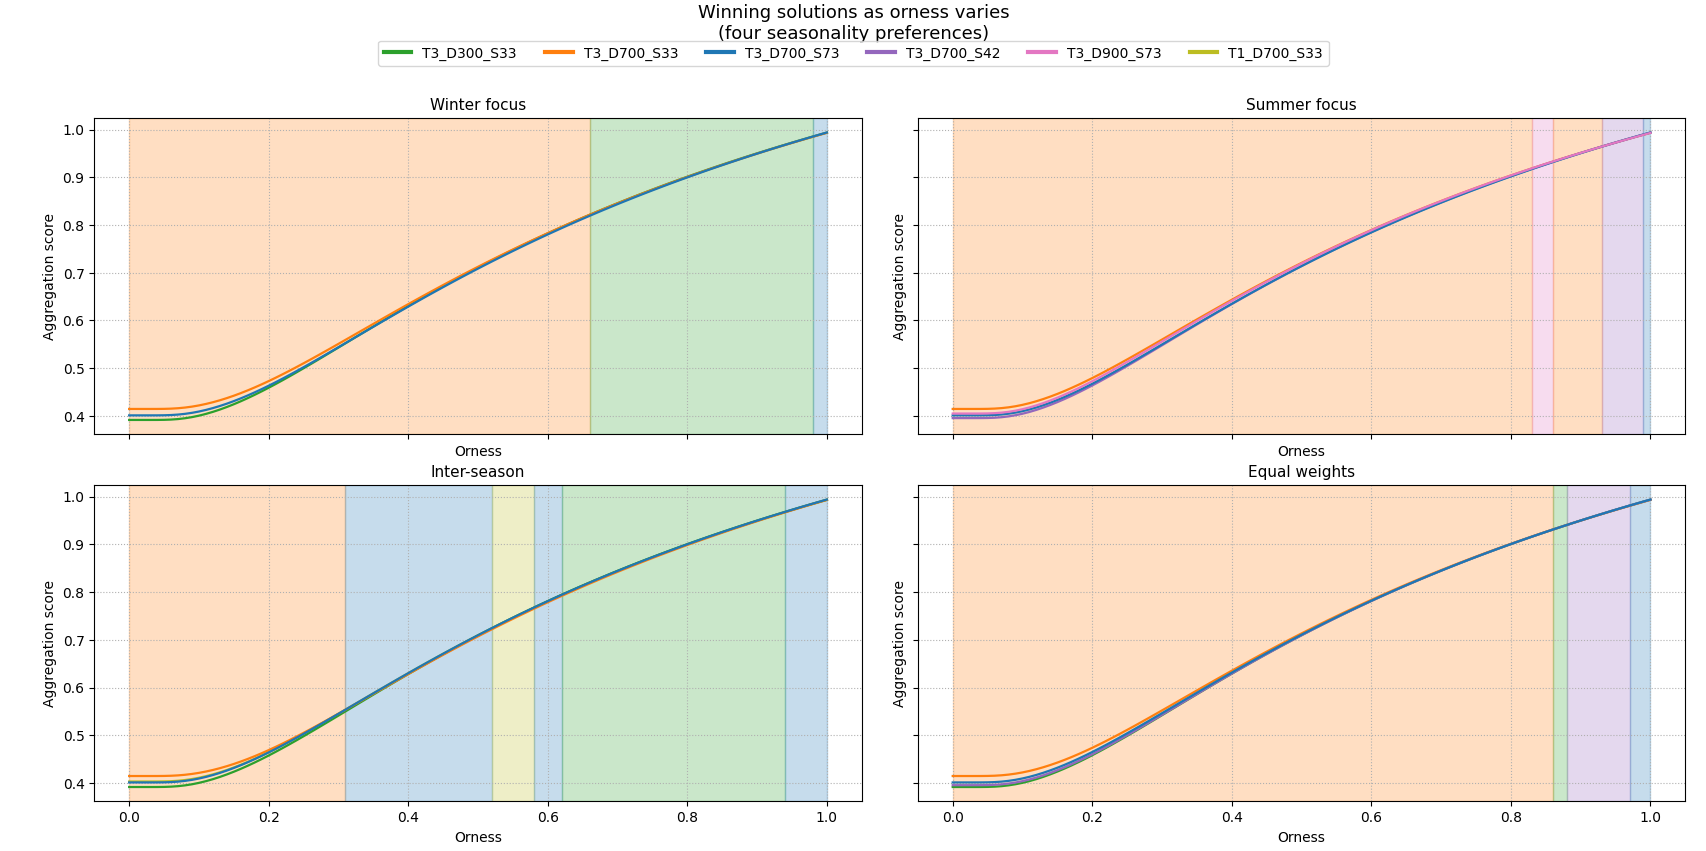
\includegraphics[width=1.08\textwidth]{ch3/figures/ResultsOrness.png}
    \end{adjustwidth}
    \caption{Final aggregation scores for the top-performing solutions across the full range of orness values ($\alpha$). Each subplot corresponds to a different seasonal preference. The colored vertical bands highlight the range of orness values for which a particular solution (identified in the legend) is optimal.}
    \label{fig:results_plot}
\end{figure}

The orness parameter, $\alpha$, critically shapes the final ranking by controlling the OWA operator's behavior. As $\alpha$ approaches 0, the aggregation mirrors a \textit{min} operator, reflecting a pessimistic or risk-averse attitude. In this regime, the decision is driven by the worst-performing attribute for each alternative. Given that the `Highest Concurrency` scores (around 0.4) are numerically much lower than the fuzzy attribute scores (all above 0.9) or seasonality (around 0.6), it becomes the dominant criterion. Consequently, for low orness values, the model consistently selects solution \texttt{T3\_D700\_S33}, as it features the most favorable (i.e., lowest) highest concurrency.\\

Conversely, as $\alpha$ approaches 1, the OWA operator emulates a \textit{max} operator, reflecting an optimistic stance that judges an alternative by its strongest attribute. In this scenario, the model favors solutions that excel in at least one key area. The results show that for high orness values, solution \texttt{T3\_D700\_S73} is predominantly chosen because it achieves the highest score in "Risk Concurrency", which represents the most uniform distribution of high-risk interventions.\\

Across the four seasonal scenarios and the entire orness spectrum, a total of seven distinct solutions emerged as optimal at some point. It is noteworthy that six of these seven top-performing solutions were generated by the algorithm from Team 3, signaling its ability to produce robust and high-quality schedules. The exception, solution \texttt{T1\_D900\_S33} from Team 1, becomes the preferred choice under the "Inter-season focus" scenario for orness values slightly above 0.5, corresponding to a moderately optimistic viewpoint. Furthermore, our epsilon-lexicographic method for handling intra-block aggregation proved effective: across 23 instances where ties occurred based on the primary criterion, the rankings were successfully resolved through consideration of the second most relevant attribute in the hierarchical structure.\\

Another relevant aspect shown in Figure \ref{fig:results_plot} is the tiny differences in the aggregated score of different solutions. This observation is further supported by the decision matrix (table \ref{tab:dm_matrix}), which reveals remarkably small variance within each column. While the heatmap (Figure \ref{fig:dif_sol}) shows that schedules can differ by hundreds of intervention start times, the attribute scores remain highly similar across solutions. This apparent contradiction is explained by how the criteria are defined and the problem's inherent constraints. The attributes are primarily dependent on the overall (shape) distribution of interventions, as all solutions must organize the exact same interventions. The highly constraints of the original problem led algorithms to naturally converge towards solutions that share a common strategy for overall workload distribution, even if they differ in specific intervention timings. Therefore, our attributes are too general and lack discriminative power, and more specific criteria focused on particular days or interventions might provide better differentiation. However, such approaches would require more detailed information than what is publicly available. The decision matrix thus captures only subtle variation of the alternatives on a common optimized approach rather than fundamentally different scheduling paradigms. \\

Due to these limitations, several avenues for future research can be suggested. A more powerful analysis could be conducted by incorporating more granular, non-public data. For instance, information on the specific economic impact of delaying certain power lines, the criticality of interventions in different geographical zones, or scenario-specific risk profiles could be used to develop more targeted criteria. Future work could also focus on designing attributes that move beyond general uniformity, such as criteria that explicitly penalize interventions during historically critical periods (e.g., Christmas days) or measure the temporal clustering of specific intervention types. Nevertheless, even with its current limitations, the proposed framework successfully provides a transparent and intuitive method for navigating these complex decisions, offering a justifiable basis for selecting a final schedule from a pool of highly competitive options. 


% Appendix
% \newpage
\appendix
% \chapter{Results from Analysis for T-norms}

\section{Continuity of T-norms}
\label{app:cont_tnorms}
T-norms are real-valued functions of two variables defined over the compact domain $[0,1]^2$ with values in $[0,1]$, and they satisfy the monotonicity property (that is, $T(x,y) \le T(x',y')$ if $x \le x'$ and $y \le y'$). These properties greatly simplify the study of their continuity. This appendix presents key results from analysis concerning the continuity and semi-continuity of t-norms\footnote{These results also apply to t-conorms, as they do not depend on one or zero identity properties.}.

\begin{notation}{Equivalence of Norms on $\R^n$}
    On a finite-dimensional vector space (like $\mathbb{R}^n$), all norms are equivalent. This is, given any two norms $\|\cdot\|_a$ and $\|\cdot\|_b$ on $\mathbb{R}^n$ satisfy

 $$
 \exists c, C > 0 \text{ such that } \forall x \in \mathbb{R}^n, \quad c\|x\|_a \leq \|x\|_b \leq C\|x\|_a.
 $$
 Since we are working on $\R^2$, the statements are equal for any given norm and we will denote it by \say{$\|\cdot\|$}.
\end{notation}

\begin{definition}[Continuity]
A t-norm $T$ is \emph{continuous at a point} $(x_0, y_0) \in [0,1]^2$ if:
\[
\forall \epsilon > 0, \exists \delta > 0 : \forall (x,y) \in [0,1]^2, \|(x,y) - (x_0,y_0)\| < \delta \implies |T(x,y) - T(x_0,y_0)| < \epsilon
\]
\end{definition}

Intuitively, this means that the value $T(x,y)$ can be made arbitrarily close to $T(x_0,y_0)$ by choosing $(x,y)$ sufficiently close to $(x_0,y_0)$. A t-norm $T$ is \emph{continuous} if it is continuous at every point in its domain $[0,1]^2$.

\begin{definition}[Uniform Continuity]
A t-norm $T$ is \emph{uniformly continuous} if:
\[
\forall \epsilon > 0, \exists \delta > 0 : \forall (x,y),(x',y') \in [0,1]^2, \|(x,y) - (x',y')\| < \delta \implies |T(x,y) - T(x',y')| < \epsilon
\]
\end{definition}
The key difference from pointwise continuity is that $\delta$ depends only on $\epsilon$, not on the specific location in the domain.
\begin{remark}
    Since the domain $[0,1]^2$ of a t-norm is a compact set, a t-norm $T$ is continuous if and only if it is uniformly continuous \cite[p.~30]{Klement2000}.
\end{remark}

Due to monotonicity, a t-norm's continuity over its 2D domain can be verified by checking continuity along its one-dimensional sections:
\begin{proposition}[Continuity via Components for Monotone Functions {\cite[Prop.~1.19]{Klement2000}}]
A t-norm $T$ (or any non-decreasing function on $[0,1]^2$) is continuous if and only if it is continuous in each variable separately. That is, for all fixed $x_0, y_0 \in [0,1]$, the functions $T(x_0, \cdot)$ and $T(\cdot, y_0)$ are continuous.
\end{proposition}

\begin{remark}
Because of the commutativity, for a t-norm
its continuity is equivalent to its continuity in the first component.\cite[p.~16]{Klement2000}
\end{remark}

\section{Semi-continuity of T-norms}
\label{app:semicont-tnorms}

Many theoretical contexts such as fuzzy logic require only less restrictive properties than continuity, such as left-continuity or upper semi-continuity. The following sections present these definitions and derive their relationships using the properties of t-norms.


\begin{definition}[Semi-continuity for T-norms {\cite[Def.~1.20]{Klement2000}}]
    A t-norm $T$ is:
    \begin{itemize}
        \item \emph{Lower semi-continuous (LSC) at $(x_0,y_0)$} if:
        \[
        \forall \epsilon > 0, \exists \delta > 0 :\, T(x,y) > T(x_0,y_0) - \epsilon \quad \forall (x,y) \in \left(]x_0 - \delta, x_0] \times ]y_0 - \delta, y_0]\right) \cap [0,1]^2
        \]
        \item \emph{Upper semi-continuous (USC) at $(x_0,y_0)$} if:
        \[
        \forall \epsilon > 0, \exists \delta > 0 :\, T(x,y) < T(x_0,y_0) + \epsilon \quad \forall (x,y) \in \left([x_0, x_0 + \delta[ \times [y_0, y_0 + \delta[\right) \cap [0,1]^2
        \]
    \end{itemize}
    A t-norm is LSC (USC) if it is LSC (USC) at every point in $[0,1]^2$.
    \end{definition}
    \begin{notation}{Topological semi-continuity}
        The definition above is only valid in metric spaces such as $\R^2$. The topological definitions are: $$T(x_0, y_0) \le \liminf_{(x,y) \to (x_0,y_0)} T(x,y) \text{ for LSC}$$   $$\text{and } T(x_0, y_0) \ge \limsup_{(x,y) \to (x_0,y_0)} T(x,y)\text{ for USC}$$
    \end{notation}
  
    Intuitively, lower semi-continuity means that the function's value does not have an isolated peak relative to its surroundings. More precisely, values $T(x,y)$ approaching from the \emph{bottom-left quadrant} are not significantly lower than $T(x_0,y_0)$. If there's a discontinuity, $T(x_0,
    y_0)$ is at the \emph{bottom} of an upward jump. Conversely, upper 
    semi-continuity means $T(x_0,y_0)$ is at the \emph{top} of a downward 
    jump.

\begin{definition}[One-Sided Continuity]
A t-norm $T$ is:
\begin{itemize}
    \item \emph{Left-continuous in its first component at $(x_0,y_0)$} if:
    \[
    \forall \epsilon > 0, \exists \delta > 0 : \, |T(x,y_0) - T(x_0,y_0)| < \epsilon \quad \forall x \in ]x_0-\delta, x_0]
    \]
    \item \emph{Right-continuous in its first component at $(x_0,y_0)$} if:
    \[
    \forall \epsilon > 0, \exists \delta > 0 :\, |T(x,y_0) - T(x_0,y_0)| < \epsilon \quad \forall x \in [x_0, x_0+\delta[, |T(x,y_0) - T(x_0,y_0)| < \epsilon
    \]
\end{itemize}
For the second component the definition is completely analogous.
$T$ is \emph{left-continuous} (or \emph{right-continuous}) if it is left-continuous (or right-continuous) in both components.
\end{definition}

\begin{remark}
    Let $T$ be a t-norm:
      \begin{align*}
        T \text{ continuous } &\Leftrightarrow T \text{ lower semi-continuous and upper semi-continuous} \\
        T \text{ continuous } &\Leftrightarrow T \text{ left-continuous and right-continuous}
      \end{align*}
\end{remark}


For general functions, semi-continuity and one-sided continuity are unrelated concepts, as semi-continuity is related to the function's range while one-sided continuity deals with domain limits. However, for monotone functions like t-norms, these properties are equivalent. This is particularly useful because one-sided continuity is often easier to establish or analyze from the construction of a t-norm.\\
\begin{proposition}[{\cite[Prop.~1.22]{Klement2000}}]
For a t-norm $T$:
\begin{itemize}
    \item $T$ is lower semi-continuous if and only if $T$ is left-continuous.
    \item $T$ is upper semi-continuous if and only if $T$ is right-continuous.
\end{itemize}
\end{proposition}

For Archimedean t-norms (those for which $T(x,x) < x$ for all $x \in ]0,1[$), an even stronger relationship between one-sided continuity and full continuity exists. This class of t-norms is fundamental in many applications.
\begin{proposition}[{\cite[Prop.~2.16]{Klement2000}}]
  For an Archimedean t-norm $T$, the following are equivalent:
  \begin{enumerate}
      \item[(i)] $T$ is left-continuous.
      \item[(ii)] $T$ is continuous.
  \end{enumerate}
\end{proposition}
This result significantly simplifies the verification of continuity for Archimedean t-norms. If such a t-norm is known to be left-continuous (e.g., due to properties of its additive or multiplicative generator, which are often easier to analyze for one-sided continuity), it is automatically fully continuous. This is a non-trivial property that does not hold for general monotone functions.

\subsection{Non-continuous T-norms}

While continuous t-norms are well-classified (section \ref{sec:class_tnorms}), not all t-norms are continuous, they can exhibit quite irregular continuity behavior:\\

The \textbf{drastic product $T_D$} is a key example of a non-continuous t-norm. It is Archimedean. It is upper semicontinuous, implying right-continuity in each variable. However, it is not left-continuous (e.g., at $(1,y)$ for $y<1$).\\

The \textbf{nilpotent minimum $T^{nM}$} is lower semicontinuous (left-continuous in each variable) but it is not right-continuous at points on the line $x+y=1$ when approached from $x+y>1$ \cite[Rem.~1.21(i)]{Klement2000}. It is defined as:
  \[
  T^{nM}(x,y) =
  \begin{cases}
    0 & \text{if } x+y \leq 1 \\
    \min(x,y) & \text{otherwise.}
  \end{cases}
  \]


The \textbf{Krause t-norm $T^K$} (\cite[App.~B.1]{Klement2000}) is a more complex example. It is constructed using the Cantor set and Farey series. It is neither left- nor right-continuous, but has a continuous diagonal section.

% \signal{
% \begin{remark}[Importance of Left-Continuity]
% For non-continuous t-norms, the property of \emph{left-continuity} (in each variable) is often a desirable, or even required, condition in certain applications, particularly in fuzzy logic. For instance, in residuum-based logics, if a t-norm $T$ is left-continuous, its corresponding residuated implication $I(x,y) = \sup\{z \in [0,1] \mid T(x,z) \le y\}$ exhibits well-behaved properties. Specifically, a commutative, integral lattice-ordered monoid based on $T$ is residuated if and only if $T$ is left-continuous (\cite[Prop.~2.47, p.~63]{Klement2000}). This ensures that the implication adequately captures deductive reasoning. While the intuitive notion that ``a microscopic decrease of the truth degree of a conjunct should not macroscopically decrease the truth degree of the conjunction" points towards continuity, left-continuity is a weaker but often sufficient condition for preserving logical coherence in such frameworks.
% \end{remark}}

\section{Generators and continuous Archimedean T-norms}
\label{app:generators_tnorms}
Continuous archimedean t-norms can be elegantly characterized and constructed through the concept of generators. 
These representations emerged from studying functional equations, particularly the associativity equation
 $T(x, T(y,z)) = T(T(x,y),z)$. The study of this equation began with N. H. Abel's work in the 19th century. J. Aczél later advanced the theory through his research on functional equations. Important insights also came from P. S. Mostert, A. L. Shields, and C. H. Ling's work on topological semigroups \cite[Sec.~5.1]{Klement2000}. Though the theory behind functional equations and topological semigroups is beyond the scope of this work, these fields were essential in developing the theory of t-norm generators.\\

The core idea of a generator is to transform the t-norm operation on $[0,1]$ into a simpler arithmetic operation on a different domain, via a strictly monotonic function. For continuous Archimedean t-norms, the additive generator provides such a framework.

An \textbf{additive generator} \cite[Def.~3.25]{Klement2000} of a t-norm $T$ is a strictly decreasing function $t: [0,1] \to [0, \infty]$ such that:
\begin{enumerate}
    \item $t(1) = 0$.
    \item $t$ is right-continuous at $0$.
\end{enumerate}
The t-norm $T$ is then constructed from its additive generator $t$ using the formula:
\begin{equation} \label{eq:additive_generator_t_norm}
    T(x,y) = t^{(-1)}( \min(t(0), t(x) + t(y)) )
\end{equation}
where $t^{(-1)}: [0, t(0)] \to [0,1]$ is the pseudo-inverse of $t$, defined as $t^{(-1)}(u) = \sup \{z \in [0,1] \mid t(z) \ge u \}$. The sum operation in equation \ref{eq:additive_generator_t_norm} is the reason why these generators are called \emph{additive}.

\begin{notation}{Multiplicative Generators}
    Parallel to additive generators, continuous Archimedean t-norms can also be represented using multiplicative generators \cite[Def.~3.36]{Klement2000}. The key differences are:
    \begin{itemize}
        \item A multiplicative generator $\theta$ is strictly \emph{increasing} (rather than decreasing)
        \item $\theta(1)=1$ (rather than $t(1)=0$)
        \item The formula analogous to Equation \ref{eq:additive_generator_t_norm} uses maximum and multiplication instead of minimum and addition:
        \[T(x,y) = \theta^{(-1)}(\max(\theta(0), \theta(x) \cdot \theta(y)))\]
        \item For strict t-norms, $\theta(0)=0$ (rather than $t(0)=\infty$)
        \item For nilpotent t-norms, $\theta(0) \in ]0,1[$ (rather than $t(0)$ finite)
    \end{itemize}
    The relationship between both types of generators is given by: \[\theta(x) = e^{-t(x)}\text{ and }t(x) = -\log(\theta(x))\]
    \end{notation}

    \begin{theorem}[Representation of Continuous Archimedean T-norms {\cite[Thm.~5.1]{Klement2000}}]
        A t-norm $T$ is a continuous Archimedean t-norm if and only if it possesses a continuous additive generator $t: [0,1] \to [0,\infty]$. This generator is unique up to a positive multiplicative constant.
      \end{theorem}
    
    This theorem is crucial because it guarantees that the entire class of continuous Archimedean t-norms can be characterized and constructed using these generator functions. Consequently, through the equivalence, they can also be represented by multiplicative generators \cite[Cor.~5.4]{Klement2000}.

The value $t(0)$ is particularly significant as it determines the nature of the continuous Archimedean t-norm \cite[Cor.~3.30]{Klement2000}:
\begin{itemize}
    \item If $t(0) = \infty$, then $\min(t(0), t(x) + t(y)) = t(x) + t(y)$, and the resulting t-norm $T$ is \textbf{strict} (e.g., for $t(x) = -\log(x)$, $T(x,y) = xy$, the product t-norm).
    \item If $t(0)$ is finite (i.e., $t(0) < \infty$), the resulting t-norm $T$ is \textbf{nilpotent} (e.g., for $t(x) = 1-x$, $T(x,y) = \max(0, x+y-1)$, the Łukasiewicz t-norm).
\end{itemize}
This representation via additive generators not only simplifies the study of continuous Archimedean t-norms but also provides a mechanism for constructing them, which is the idea behind the families of t-norms. The general approach involves:
\begin{enumerate}
    \item Starting with a known generator function. For example:
    \begin{itemize}
        \item $t_L(x) = 1-x$, the additive generator for the Łukasiewicz t-norm ($T_L$).
        \item $t_P(x) = -\log x$, the additive generator for the Product t-norm ($T_P$).
    \end{itemize}
    \item Introducing one or more parameters (often denoted by $\lambda, p, \dots$) into the structure of this generator function to create a parameterized generator $t_\lambda(x)$.
    \item Applying the construction formula (Equation~\eqref{eq:additive_generator_t_norm}) with $t_\lambda(x)$ to obtain a parametric family of t-norms $T_\lambda(x,y)$.
\end{enumerate}
The properties of the resulting t-norm family (e.g., whether its members are strict or nilpotent, their continuity with respect to the parameter) depend on how the parameter affects $t_\lambda(0)$ and the overall shape of $t_\lambda$. Many well-known t-norm families are derived in this manner.


\begin{example}[Examples of T-norm Families]\label{ex:families_tnorms}
    Below are some families of continuous Archimedean t-norms, along with their definitions and key generator properties. These are extracted from \cite[App.~A]{Klement2000}.

    \textbf{1. Schweizer-Sklar T-norms} ($T_\lambda^{SS}$) for $\lambda \in [-\infty, \infty]$ 
\begin{itemize}
    \item $T_\lambda^{SS}(x,y) = \begin{cases} T_M(x,y) & \text{if } \lambda = -\infty \\ T_P(x,y) & \text{if } \lambda = 0 \\ T_D(x,y) & \text{if } \lambda = \infty \\ (\max(x^\lambda + y^\lambda - 1, 0))^{1/\lambda} & \text{if } \lambda \in ]-\infty, 0[ \cup ]0, \infty[ \end{cases}$
    \item Additive generator (for $\lambda \in ]-\infty, 0[ \cup ]0, \infty[$): $t_\lambda^{SS}(x) = \frac{1-x^\lambda}{\lambda}$ (if $\lambda=0$, $t_0^{SS}(x) = -\log x$).
    \item $t_\lambda^{SS}(0) = \infty$ for $\lambda \in ]-\infty, 0]$, hence $T_\lambda^{SS}$ is strict.
    \item $t_\lambda^{SS}(0) = \frac{1}{\lambda} < \infty$ for $\lambda \in ]0, \infty[$, hence $T_\lambda^{SS}$ is nilpotent. ($T_\infty^{SS} = T_D$ is not Archimedean).
\end{itemize}

\textbf{2. Hamacher T-norms} ($T_\lambda^H$) for $\lambda \in [0, \infty]$ 
\begin{itemize}
    \item $T_\lambda^H(x,y) = \begin{cases} T_D(x,y) & \text{if } \lambda = \infty \text{ and } (x,y) \neq (0,0) \\ 0 & \text{if } \lambda = \infty \text{ and } x=y=0 \\ \frac{xy}{\lambda + (1-\lambda)(x+y-xy)} & \text{if } \lambda \in [0, \infty[ \end{cases}$
    (Note: $T_0^H = T_P$)
    \item Additive generator (for $\lambda \in [0, \infty[$): $t_\lambda^H(x) = \log\left(\frac{\lambda + (1-\lambda)x}{x}\right)$ (if $\lambda=0$, $t_0^H(x)=\frac{1-x}{x}$).
    \item $t_\lambda^H(0) = \infty$ for all $\lambda \in [0, \infty[$, hence $T_\lambda^H$ is strict.
\end{itemize}

\textbf{3. Frank T-norms} ($T_\lambda^F$) for $\lambda \in [0, \infty]$ 
\begin{itemize}
    \item $T_\lambda^F(x,y) = \begin{cases} T_M(x,y) & \text{if } \lambda = 0 \\ T_P(x,y) & \text{if } \lambda = 1 \\ T_L(x,y) & \text{if } \lambda = \infty \\ \log_\lambda \left(1 + \frac{(\lambda^x-1)(\lambda^y-1)}{\lambda-1}\right) & \text{if } \lambda \in ]0, 1[ \cup ]1, \infty[ \end{cases}$
    \item Additive generator (for $\lambda \in ]0, 1[ \cup ]1, \infty[$): $t_\lambda^F(x) = \log_\lambda \left(\frac{\lambda^x-1}{\lambda-1}\right)$. (For $\lambda=1$, $t_1^F(x) = -\log x$; for $\lambda=\infty$, $t_\infty^F(x) = 1-x$).
    \item $t_\lambda^F(0) = \infty$ for $\lambda \in [0, \infty[$, hence $T_\lambda^F$ is strict.
    \item $t_\infty^F(0) = 1 < \infty$, hence $T_\infty^F = T_L$ is nilpotent.
\end{itemize}

\textbf{4. Yager T-norms} ($T_\lambda^Y$) for $\lambda \in [0, \infty]$
\begin{itemize}
    \item $T_\lambda^Y(x,y) = \begin{cases} T_D(x,y) & \text{if } \lambda = 0 \\ T_M(x,y) & \text{if } \lambda = \infty \\ \max\left(1 - ((1-x)^\lambda + (1-y)^\lambda)^{1/\lambda}, 0\right) & \text{if } \lambda \in ]0, \infty[ \end{cases}$
    (Note: $T_1^Y = T_L$)
    \item Additive generator (for $\lambda \in ]0, \infty[$): $t_\lambda^Y(x) = (1-x)^\lambda$.
    \item $t_\lambda^Y(0) = 1 < \infty$ for all $\lambda \in ]0, \infty[$, hence $T_\lambda^Y$ is nilpotent.
\end{itemize}

\textbf{5. Dombi T-norms} ($T_\lambda^D$) for $\lambda \in [0, \infty]$ 
\begin{itemize}
    \item $T_\lambda^D(x,y) = \begin{cases} T_D(x,y) & \text{if } \lambda = 0 \\ T_M(x,y) & \text{if } \lambda = \infty \\ \frac{1}{1 + \left(\left(\frac{1}{x}-1\right)^\lambda + \left(\frac{1}{y}-1\right)^\lambda\right)^{1/\lambda}} & \text{if } \lambda \in ]0, \infty[ \text{ (for } x,y > 0) \end{cases}$
    ($T(x,0)=T(0,x)=0$ for $x \in$). (Note: $T_1^D = T_H$ with parameter $\gamma=1$, the Hamacher product)
    \item Additive generator (for $\lambda \in ]0, \infty[$): $t_\lambda^D(x) = \left(\frac{1-x}{x}\right)^\lambda$.
    \item $t_\lambda^D(0) = \infty$ for all $\lambda \in ]0, \infty[$, hence $T_\lambda^D$ is strict.
\end{itemize}

\textbf{6. Sugeno-Weber T-norms} ($T_\lambda^{SW}$) for $\lambda \in [-1, \infty]$
\begin{itemize}
    \item $T_\lambda^{SW}(x,y) = \begin{cases} T_D(x,y) & \text{if } \lambda = -1 \\ T_P(x,y) & \text{if } \lambda = \infty \\ \max\left(\frac{x+y-1+\lambda xy}{1+\lambda}, 0\right) & \text{if } \lambda \in ]-1, \infty[ \end{cases}$
    (Note: $T_0^{SW} = T_L$)
    \item Additive generator (for $\lambda \in ]-1, \infty[$): $t_\lambda^{SW}(x) = 1 - \frac{\log(1+\lambda x)}{\log(1+\lambda)}$. (For $\lambda=0$, $t_0^{SW}(x)=1-x$; for $\lambda \to \infty$, $t_\infty^{SW}(x)=-\log x$).
    \item $t_\lambda^{SW}(0) = 1 < \infty$ for $\lambda \in ]-1, \infty[$, hence $T_\lambda^{SW}$ is nilpotent.
    \item $t_\infty^{SW}(0) = \infty$, hence $T_\infty^{SW} = T_P$ is strict.
\end{itemize}

\textbf{7. Aczél-Alsina T-norms} ($T_\lambda^{AA}$) for $\lambda \in [0, \infty]$
\begin{itemize}
    \item $T_\lambda^{AA}(x,y) = \begin{cases} T_D(x,y) & \text{if } \lambda = 0 \\ T_M(x,y) & \text{if } \lambda = \infty \\ e^{-\left((-\log x)^\lambda + (-\log y)^\lambda\right)^{1/\lambda}} & \text{if } \lambda \in ]0, \infty[ \end{cases}$
    (Note: $T_1^{AA} = T_P$)
    \item Additive generator (for $\lambda \in ]0, \infty[$): $t_\lambda^{AA}(x) = (-\log x)^\lambda$.
    \item $t_\lambda^{AA}(0) = \infty$ for all $\lambda \in ]0, \infty[$, hence $T_\lambda^{AA}$ is strict.
\end{itemize}
\end{example}


\chapter{Propositional logic and algebraic logic.}

This appendix provides essential context and key concepts for understanding the connection between logic and algebra. While comprehensive coverage of all details is beyond scope, the focus remains on building intuition about what formal logic is and what it means for a logic to possess algebraic structure. 

\subsection*{Brief History}

The study of understanding and formalizing reasoning\footnote{This subsection is based on \cite[p.~5-8]{ConciseLogicBook} with some additional comments regarding Peano, Hilbert and Tarski from \cite{MathLogicBook}.} began in ancient Greece with Aristotle's work on syllogisms, which provided the foundation for deductive reasoning for nearly two millennia. The Stoic philosophers also made significant early contributions to what we now recognize as propositional logic, though much of their work was lost to time. While Leibniz later envisioned a universal formal language for reasoning, it wasn't until the 19th century that modern mathematical logic truly emerged.\\

The field saw major developments through Boole's algebra of logic, De Morgan's work on relations, and most crucially, Frege's introduction of predicate logic with quantification in his Begriffsschrift (1879). This period was driven by a need for greater mathematical rigor, especially in analysis and geometry. Peano further contributed by developing formal axioms for arithmetic and emphasizing logical symbolism in proofs.\\

The early 20th century brought both ambitious hopes and fundamental limitations. While Russell and Whitehead attempted to derive all mathematics from logic in Principia Mathematica and Hilbert proposed his program for securing mathematical foundations, Gödel's incompleteness theorems (1931) revealed inherent limitations to formal systems. Tarski's work on semantics and truth later provided crucial tools for understanding formal languages and their models.\\

\section{Formal Logic}
\label{app:form_log}

As Hájek states: \say{Logic studies the notion(s) of consequence. [...] The task of formal logic is to represent all this by means of well-defined
logical calculi admitting exact investigation}\cite[p.1]{Hajek1998}. A formal logic provides a precise framework for reasoning. Examples of formal logics are:

\begin{itemize}
    \item Propositional logic (PL, also called Sentential logic)\cite[Ch.~6]{ConciseLogicBook}: it deals with statements (propositions) and combinations of them through connectives ($ \lor, \land, \neg, \rightarrow, \leftrightarrow$).
    \item First Order Logic (also called Predicate logic)\cite[Ch.~8]{ConciseLogicBook}: extends propositional logic by introducing predicates, terms (names and variables over individual domains), and quantifiers ($\forall$, $\exists$) to make general statements about these individuals. As stated in \cite[p.~67]{MathLogicBook}, when the ''working mathematician" finds a proof, it is almost invariably meant to be one that can be formalized in First Order Logic.
    \item Other families of formal logics often build upon, extend, or modify the principles of propositional or predicate logic. Some examples include: modal logics, temporal logics, intuitionistic logic and many-valued logics.
\end{itemize}

Continuing with the cites from Hájek \cite[p.1]{Hajek1998}: \say{Often a logical calculus has two notions of consequence: syntactical (based on a notion of proof) and semantical (based on a notion of truth); then the natural questions of soundness (does provability imply truth?) and completeness (does truth imply provability?) pose themselves.} A formal logic is typically characterized by its syntax, semantics, and a proof system.

\paragraph{Syntax} defines the formal language: its vocabulary of basic symbols (like propositional variables $P, Q$ and connectives $\neg, \rightarrow$) and formation rules for constructing well-formed formulas (WFFs)\footnote{This can be understood as grammar. It is just to exclude formulas that are incorrect. Some examples that don't make sense and wouldn't be considered WFF are: "$))P\Rightarrow \neg\Rightarrow $" or "$P \land \Leftarrow \lor Q$".\cite[Sec.~2.3.3]{Agler2013SymbolicLogic}} (e.g., $(P \rightarrow Q)$ in PL \cite[Sec.~2.3.3]{Agler2013SymbolicLogic}).

\begin{figure}[!ht]
    \centering
    \resizebox{\textwidth}{!}{%
    \begin{tikzpicture}[node distance=1cm and 2.5cm]
        
        \node[title] (title_syntax) {Syntax: Propositional to Predicate Logic}; 
    
        \node[block, below=0.5cm of title_syntax, xshift=-1cm] (prop_syntax) {
            \textbf{Propositional Logic Syntax}
            \begin{itemize}
                \setlength\itemsep{0em}
                \item Propositional Variables ($P, Q$)
                \item Truth Constants (e.g., $\bar{0}, \bar{1}$)
                \item Logical Connectives ($\Rightarrow$, $\land$, $\lor$, $\neg$)
                \item Formation Rules for WFFs
            \end{itemize}
        };
    
        \node[block_ext, right=of prop_syntax] (pred_syntax) {
            \textbf{FOL Syntax (Extends Propositional)}

            \textcolor{pastelred!70!black}{\textit{All Propositional Syntax Elements plus:}}
            \begin{itemize}
                \setlength\itemsep{0em}
                \item Object Symbols: Variables ($x$), Constants ($c$)
                \item Structure Symbols: Predicates ($P(\cdot)$), Functions ($f(\cdot)$)
                \item Quantifiers ($\oldforall, \exists$)
                \item Terms (functions on objects)
                \item Atomic Formulas (predicates on terms)
                \item Extended Formation Rules for WFFs
            \end{itemize}
        };
        \path [line] (prop_syntax.east) -- (pred_syntax.west) node [midway, above, font=\footnotesize] {Extends with};
    \end{tikzpicture}}
    \caption{Syntax elements for propositional logic and their extension in first-order logic. Based on \cite[Ch.~2,5]{Hajek1998}.}
    \label{fig:syntax_diagram}
    \end{figure}

\paragraph{Semantics} assigns meaning to these WFFs, primarily by defining how truth is determined. For classical propositional logic, this involves assigning truth values (True or False) to atomic propositions and the meaning of the logical connectives, often illustrated using truth tables \cite[Sec.~3.1-3.2]{Agler2013SymbolicLogic}. Each distinct assignment of truth values to atomic propositions constitutes a model \cite[Sec.~3.1]{Agler2013SymbolicLogic}. A WFF is semantically valid (e.g., a tautology in PL \cite[Sec.~3.3.1]{Agler2013SymbolicLogic}) if it is true in all possible models. For predicate logic, semantics include as well interpretations over a domain of discourse, assigning objects to names and sets of objects (or n-tuples) to predicates \cite[Ch.~6.4]{Agler2013SymbolicLogic}.

\begin{figure}[!ht]
    \centering
    \resizebox{\textwidth}{!}{%
    \begin{tikzpicture}[node distance=1cm and 2.5cm]
        \node[title] (title_sem) {Semantics: Propositional to Predicate Logic};
        \node[block, below=0.5cm of title_sem, xshift=-1cm] (prop_sem) {
            \textbf{Propositional Logic Semantics}
            \begin{itemize}
                \setlength\itemsep{0em}
                \item Truth Value Algebra $\mathbf{L}$ (e.g., $[0,1]$ with t-norm, residuum)
                \item Evaluation $e$: assigns truth values to propositional variables
                \item Truth functions for connectives
            \end{itemize}
        };
        \node[block_ext, right=of prop_sem] (pred_sem) {
            \textbf{FOL Semantics (Extends Propositional)}

            \textcolor{pastelred!70!black}{\textit{Same Truth Value Algebra plus:}}
            \begin{itemize}
                \setlength\itemsep{0em}
                \item Domain of Discourse $U$
                \item Interpretation (Model) $\mathcal{M}$ maps:
                    \begin{itemize}
                    \setlength\itemsep{0em}
                        \item Constants $\rightarrow$ elements in $U$
                        \item Function symbols $\rightarrow$ functions on $U$
                        \item Predicate symbols $\rightarrow$ fuzzy relations on $U$ ($r_P: U^n \to \mathbf{L}$)
                    \end{itemize}
                \item Variable Assignment $v: \text{ObjVars} \to U$
                \item Truth for atomic formulas via fuzzy relations
                \item Truth for connectives (as propositional)
                \item Truth for quantifiers (inf/sup over domain)
            \end{itemize}
        };
        \path [line] (prop_sem.east) -- (pred_sem.west) node [midway, above, font=\footnotesize] {Extends with};
    \end{tikzpicture}}
    \caption{Diagram summarizing the extension of semantics from fuzzy propositional logic to fuzzy predicate logic. Based on the ideas from \cite[Ch.~2,5]{Hajek1998}.}
    \label{fig:semantics_diagram}
    \end{figure} 

\paragraph{Proof System (or Deductive System)} provides a way to derive WFFs from other WFFs. It consists of axioms (if any) and rules of inference (like Modus Ponens\footnote{Some formal logics such as Hilbert Systems, rely on having a sufficiently expressive set of axioms and Modus Ponens as their only rule of inference then other rules can be deduced\cite[Sec.~1.2, Def.~1.2.6]{Hajek1998}. Hilbert Systems can be used to define Classical Propositional Logics satisfying completeness. In general, more rules may be defined as well, such as the substitution rule in Gentzen Calculus for intuitionistic logic. \cite[p.~39]{ResiduatedLattices2007}}) \cite[Sec.~5.1, 5.3]{Agler2013SymbolicLogic}. A proof is a finite sequence of WFFs where each WFF is an axiom, a premise (an assumption for the specific argument), or follows from preceding WFFs in the sequence by a rule of inference \cite[Sec.~5.1]{Agler2013SymbolicLogic}. A formula $\phi$ is provable from a set of premises $\Gamma$ (written $\Gamma \vdash \phi$) if such a proof exists. If $\phi$ is provable from no premises ($\vdash \phi$), i.e. using only the axioms without specific assumptions, it is called a theorem of the logic.\\

The fundamental goal of a logical system is to align its syntactic derivations with semantic truth. This is represented by two properties of a formal logic: soundness ensures that only valid formulas are provable ($\vdash \phi \implies \models \phi$), while completeness ensures that all valid formulas are provable ($\models \phi \implies \vdash \phi$) \cite[Lemmas~1.2.7, 1.2.9]{Hajek1998}. When a logic is both sound and complete, provability and validity become equivalent concepts. Semantic truth is achievable through syntactic manipulation.\cite[Thm.~1.2.11]{Hajek1998}




\section{Algebraic Logic}
\label{app:alg_log}
Algebraic logic investigates the connections between logical systems and algebraic structures, a field advanced by Tarski's work on propositional formulas \cite[p.~1]{BlokPigozzi1989}. \signal{The key insight is that provable statements and logical equivalences within a deductive system correspond to properties of operations in algebraic structures.} For example, classical propositional logic maps directly to Boolean algebras. This relationship can be understood through both the syntax (proof theory) and semantics (model theory) of a logic.

\paragraph{From the Syntactic Side} For propositional logics, we can construct a canonical algebraic structure called the \textbf{Lindenbaum-Tarski algebra}. The process begins by grouping formulas into equivalence classes. Two formulas, $\phi$ and $\psi$, are considered equivalent (and belong to the same class, denoted $[\phi]$) if they are provably interchangeable within the logic, i.e., $\vdash (\phi \leftrightarrow \psi)$. This notion of equivalence must be compatible with the logical connectives, meaning $\leftrightarrow$ behaves as a congruence relation \cite[p.~1-2]{BlokPigozzi1989}. The logical connectives (e.g., $\wedge, \lor, \rightarrow$) then naturally induce operations on these equivalence classes (for example, $[\phi] \bar{\wedge} [\psi] = [\phi \wedge \psi]$).

The specific type of algebraic structure that results (e.g., a Boolean algebra for classical propositional logic, or a Heyting algebra for intuitionistic logic \cite[Ch.~1]{ResiduatedLattices2007}) is entirely determined by the axioms and inference rules of the logic itself. In this algebra, a formula $\phi$ is a theorem of the logic ($\vdash \phi$) if and only if its equivalence class $[\phi]$ is the ''top" element (often denoted $1$ or $\top$), representing provable truth. The Lindenbaum-Tarski algebra is, in a specific sense, the ''most general" algebraic model for the logic, as it satisfies precisely those algebraic laws corresponding to the logic's theorems and no others.

\paragraph{From the Semantic Side} We can define the meaning or interpretation of a logic by choosing a class of algebraic structures, $\mathcal{K}$, to serve as its models.\footnote{A class $\mathcal{K}$ is typically a collection of algebraic structures that share the same signature (sets of operations with same ary) and satisfy common defining properties. Often, $\mathcal{K}$ forms a \textit{variety} (defined by equations) or a \textit{quasivariety} (defined by quasi-equations) \cite[Def.~2.2]{BlokPigozzi1989}.}

The elements of an algebra $A \in \mathcal{K}$ are the truth values. For classical propositional logic, this is typically the two-element Boolean algebra $\mathbf{2} = (\{0,1\}, \land, \lor, \neg, 0, 1)$. For many fuzzy logics, the truth values come from the real unit interval $[0,1]$, equipped with suitable operations like t-norms and their residua \cite[Ch.~2]{Hajek1998}.

A \textit{valuation} (or interpretation) $v$ is a homomorphism from the algebra of formulas into an algebra $A \in \mathcal{K}$. This means $v$ maps propositional variables to elements of $A$ and preserves operations corresponding to connectives. A formula $\phi$ is a $\mathcal{K}$\textbf{-tautology} if $v(\phi)$ evaluates to a designated ''true" value (typically $1$) for all valuations $v$ into every algebra $A \in \mathcal{K}$. For fuzzy logics, these are often called $1$-tautologies \cite[Ch.~2]{Hajek1998}.

\paragraph{Bridging Syntax and Semantics} The crucial link between both approaches is established through soundness and completeness theorems. A logic is \textbf{sound} with respect to a class of algebras $\mathcal{K}$ if every provable formula is a $\mathcal{K}$-tautology. It is \textbf{complete} if every $\mathcal{K}$-tautology is a theorem.

When a logic is sound and complete with respect to $\mathcal{K}$, its Lindenbaum-Tarski algebra is characteristically embedded within $\mathcal{K}$. This means that logical consequence can be effectively translated into equational consequence within $\mathcal{K}$ \cite[Abstract]{BlokPigozzi1989}. Logics with particularly strong and well-defined translations between logical deduction and algebraic reasoning are termed \textbf{algebraizable} \cite[Def.~2.10]{BlokPigozzi1989}.\\

For example, Hájek's Basic Logic (BL) \cite[Ch.~2]{Hajek1998} is complete with respect to the class of all linearly ordered BL-algebras \cite[Thm.~2.3.15]{Hajek1998}. However, BL is \textit{not} complete with respect to the \textit{single} standard Łukasiewicz algebra on $[0,1]$. The formula $\neg \neg \phi \leftrightarrow \phi$ (double negation elimination) is a tautology in this particular algebra but not provable in BL. Thus, the Lindenbaum-Tarski algebra of BL does not satisfy $\neg \neg x = x$, while the standard Łukasiewicz algebra does. This illustrates that the Lindenbaum-Tarski algebra of BL is more general, validating only what is provable in BL, and that completeness often requires a broader class of algebraic models.\\

For semantic purposes (defining truth, checking validity), it's often simpler to work with concrete algebras of truth values rather than directly with the (often infinite and complex) Lindenbaum-Tarski algebra of equivalence classes. Soundness and completeness theorems allow us to do so by showing that provability (tied to the Lindenbaum-Tarski algebra) corresponds to validity in these (often simpler) algebraic models.\\

\signal{It is essentially what you get if you ''quotient" the $L_T$ algebra by its relationship with truth.}\\

\signal{I think that $\mathcal{K}$ contains $L_T$ when we have soundness and completeness.}

\signal{De aquí para adelante en el apéndice tengo que repasarlo bien y resumir y demás, solo he puesto cosas de libros sin redactar del todo bien.}

This algebraic perspective is particularly fruitful for fuzzy logics, where the truth values are typically ordered and often continuous\footnote{\signal{For non-continuous see perfect MV-algebras.}}. The algebraic study of fuzzy logics has identified several important classes of ordered algebraic structures, many of which are based on the real unit interval $[0,1]$ as the set of truth values:
\begin{itemize}
    \item \textbf{Residuated Lattices}: These form a very general algebraic foundation for a wide range of fuzzy and substructural logics. They combine a lattice structure (for conjunction $\wedge$ and disjunction $\vee$) with a monoid operation $\otimes$ (modeling a strong, typically conjunctive, connective, often a t-norm) and its residuum $\rightarrow$ (modeling implication). These operations are linked by the adjointness property: $x \otimes y \leq z \iff x \leq y \rightarrow z$, which captures a fundamental deductive relationship.
    \item \textbf{MTL-algebras (Monoidal t-norm based Logic algebras)}: These are residuated lattices that are also prelinear (i.e., they satisfy the condition $(x \rightarrow y) \vee (y \rightarrow x) = 1$, reflecting a total order of truth values or a linear framework for comparing implications). They serve as the algebraic counterparts of Monoidal t-norm Logic (MTL), which axiomatizes the tautologies common to all logics based on left-continuous t-norms and their residua.
    \item \textbf{BL-algebras (Basic Logic algebras)}: These are MTL-algebras that additionally satisfy the divisibility condition: $x \wedge y = x \otimes (x \rightarrow y)$. They are the algebraic semantics for Basic Logic (BL), which is the logic of all continuous t-norms and their residua.
    \item \textbf{MV-algebras (Łukasiewicz Logic algebras)}: These are BL-algebras that are also involutive, meaning they satisfy $\neg \neg x = x$ (where the negation is defined as $\neg x = x \rightarrow 0$, with $0$ being the bottom element). They are the algebraic semantics for Łukasiewicz logic, which is based on the Łukasiewicz t-norm.
    \item \textbf{Gödel algebras (G-algebras)}: These are BL-algebras where the monoidal operation $\otimes$ is idempotent ($x \otimes x = x$), which implies that $\otimes$ coincides with the lattice meet operation $\wedge$. They correspond to Gödel logic, based on the minimum t-norm. Gödel algebras are a subclass of Heyting algebras (the algebraic semantics for intuitionistic logic).
    \item \textbf{Product algebras ($\Pi$-algebras)}: These are BL-algebras satisfying specific additional axioms that characterize product logic, which is based on the algebraic product t-norm.
\end{itemize}
















\subsection{Substructural Logics and Residuated Lattices}

Many logics, including classical and intuitionistic logic, satisfy certain ''structural rules" in their Gentzen-style formulations, such as:
\begin{itemize}
    \item \textbf{Weakening:} Allows adding arbitrary formulas to antecedents or succedents.
    \item \textbf{Contraction:} Allows replacing multiple occurrences of a formula with a single one.
    \item \textbf{Exchange:} Allows reordering formulas.
\end{itemize}
\textbf{Substructural logics} are logics where one or more of these structural rules are restricted or absent. Examples include relevance logics (lack weakening), linear logic (lacks weakening and contraction), and fuzzy logics.

The algebraic study of substructural logics reveals that their algebraic counterparts are often \textbf{residuated lattices} (or related structures).
A residuated lattice is, at its core, a lattice $(L, \land, \lor)$ equipped with a monoid operation $\cdot$ (fusion) and two binary operations $\backslash$ (left residual) and $/$ (right residual) satisfying the residuation property:
\[ x \cdot y \le z \iff y \le x \backslash z \iff x \le z / y \]
This is a generalization of the relationship in Heyting algebras ($x \land y \le z \iff y \le x \to z$) where fusion is meet, and the implication $\to$ is the residual. In Boolean algebras, $x \cdot y = x \land y$ and $x \to y = \neg x \lor y$. The implication $\to$ in logics often corresponds to a residual operation.
The absence or presence of structural rules in the logic corresponds to specific algebraic properties of the residuated lattices (e.g., commutativity of $\cdot$ for exchange, integrality for weakening, idempotence of $\cdot$ for contraction).



\subsection{Characteristics and Intuitions of Foundational Fuzzy Logics}

The foundational logics—MTL, BL, $\L$, G, and $\Pi$—form a hierarchy: MTL is most general, based on all left-continuous t-norms and their residua; BL restricts to continuous t-norms; and each of $\L$, G, $\Pi$ is a further axiomatic specialization of BL connected to a distinguished continuous t-norm.

\begin{itemize}
    \item \textbf{Generality}: MTL omits the divisibility property ($x*(x \Rightarrow y)=\min(x,y)$), so min-conjunction is not definable from strong conjunction and implication; BL recovers it for continuous t-norms.
    \item \textbf{Negation}: $\L$ has involutive (double) negation, G and $\Pi$ use a Gödel-type negation, while MTL and BL only ensure weaker forms (involutive negation may be added as an axiom for special subclasses like IMTL~\cite{GodoMonoidal}).
    \item \textbf{Nature of conjunction (t-norm)}:
        \begin{itemize}
            \item $\L$: Additive-like, compensatory.
            \item G: Minimum, conservative (weakest link/idempotent).
            \item $\Pi$: Product, multiplicative.
        \end{itemize}
    \item \textbf{Deduction theorem}: G has a stronger deduction theorem than the others; in $\L$, $\Pi$, BL, and MTL, only a weaker, ''n-fold" deduction theorem holds.
    \item \textbf{Completeness}: BL, $\L$, G, and $\Pi$ are complete with respect to their standard [0,1] semantics as based on continuous t-norms. MTL is complete w.r.t.\ linearly ordered MTL-algebras and, non-trivially, for the left-continuous t-norms~\cite{Jenei2001MTLCompl}. G has full (not only 1-tautology) completeness for arbitrary theories~\cite[Thm. 4.2.17]{Hajek1998}; completeness of BL and $\L$ is for 1-tautologies, and extensions vary.
    \item \textbf{Relationship to classical logic}: Pairwise combinations of $\L$, G, and $\Pi$ generate classical logic~\cite[Thm. 4.3.9]{Hajek1998}.
\end{itemize}
Each logic is therefore tailored for different reasoning needs. MTL, as the most general, accommodates any left-continuous t-norm and provides the universal backbone for fuzzy deduction systems.

% \rule{\textwidth}{0.4mm}


% A formal logic is typically characterized by its syntax, semantics, and a proof system.

% \paragraph{Syntax} defines the formal language: its vocabulary of basic symbols and rules for constructing well-formed formulas (WFFs)\footnote{This can be understood as grammar. It is just to exclude formulas that are incorrect. Some examples that don't make sense and wouldn't be considered WFF are: "$))P\Rightarrow \neg\Rightarrow $" or "$P \land \Leftarrow \lor Q$".\cite[Sec.~2.3.3]{Agler2013SymbolicLogic}}. Figure~\ref{fig:syntax_diagram} illustrates these components. Propositional logic (PL) syntax (left in Fig.~\ref{fig:syntax_diagram}) includes propositional variables (e.g., $P, Q$) and logical connectives (e.g., $\neg, \rightarrow$) used to form WFFs like $(P \rightarrow Q)$ \cite[Sec.~2.3.3]{Agler2013SymbolicLogic}. First-order logic (FOL) syntax (right in Fig.~\ref{fig:syntax_diagram}) extends PL by adding new vocabulary such as object variables (e.g., $x,y$), object constants (e.g., $c,d$), predicate symbols (e.g., $P(-)$), function symbols (e.g., $f(-)$), and quantifiers ($\forall, \exists$). From variables, constants, and function applications, a syntactic category called \textit{terms} is formed; these generally refer to objects. \textit{Atomic formulas} are then constructed by applying predicate symbols to terms. These, along with the propositional connectives and quantifiers, are used in the extended formation rules to build complex WFFs.

% \begin{figure}[!ht]
%     \centering
%     \resizebox{\textwidth}{!}{%
%     \begin{tikzpicture}[node distance=1cm and 2.5cm]
        
%         \node[title] (title_syntax) {Syntax: Propositional to Predicate Logic}; 
    
%         \node[block, below=0.5cm of title_syntax, xshift=-1cm] (prop_syntax) {
%             \textbf{Propositional Logic Syntax}
%             \begin{itemize}
%                 \setlength\itemsep{0em}
%                 \item Propositional Variables ($P, Q$)
%                 \item Truth Constants (e.g., $\bar{0}, \bar{1}$)
%                 \item Logical Connectives (\&, $\rightarrow$, $\land$, $\lor$, $\neg$)
%                 \item Formation Rules for WFFs
%             \end{itemize}
%         };
    
%         \node[block_ext, right=of prop_syntax] (pred_syntax) {
%             \textbf{First-Order Logic Syntax (Extends Propositional)}
%             \begin{itemize}
%                 \setlength\itemsep{0em}
%                 \item \textcolor{pastelred!70!black}{\textit{All Propositional Syntax Elements plus:}}
%                 \item Object Symbols: Variables ($x$), Constants ($c$)
%                 \item Structure Symbols: Predicates ($P(\cdot)$), Functions ($f(\cdot)$)
%                 \item Quantifiers ($\oldforall, \exists$)
%                 \item Terms (functions on objects)
%                 \item Atomic Formulas (predicates on terms)
%                 \item Extended Formation Rules for WFFs
%             \end{itemize}
%         };
%         \path [line] (prop_syntax.east) -- (pred_syntax.west) node [midway, above, font=\footnotesize] {Extends with};
%     \end{tikzpicture}}
%     \caption{Syntax elements for propositional logic and their extension in first-order logic. Based on \cite[Ch.~2,5]{Hajek1998}.}
%     \label{fig:syntax_diagram}
%     \end{figure}

% \paragraph{Semantics} assigns meaning to WFFs, primarily by defining how their truth is determined. Key semantic components are outlined in Figure~\ref{fig:semantics_diagram}. For propositional logic (left in Fig.~\ref{fig:semantics_diagram}), this involves a truth-value algebra (e.g., classical \{True, False\}, or a continuous range like $[0,1]$ for many-valued logics), an evaluation function $e$ assigning truth values from this algebra to propositional variables, and truth functions defining how connectives operate on these values (often given by truth tables in classical PL \cite[Sec.~3.1-3.2]{Agler2013SymbolicLogic}). A specific assignment of truth values to atomic propositions constitutes a model (or valuation \cite[Sec.~3.1]{Agler2013SymbolicLogic}). A WFF is semantically valid (a tautology in PL \cite[Sec.~3.3.1]{Agler2013SymbolicLogic}) if true in all models. As Figure~\ref{fig:semantics_diagram} (right) shows, first-order logic semantics extends this framework. It introduces a domain of discourse $U$ and an interpretation $\mathcal{M}$ that maps constants to elements in $U$, function symbols to functions on $U$, and predicate symbols to relations on $U$ \cite[Ch.~6.4]{Agler2013SymbolicLogic}. A variable assignment $v$ maps object variables to elements in $U$. The truth of quantified formulas is typically defined using infima/suprema over the domain elements.


% \begin{figure}[h!]
%     \centering
%     \resizebox{\textwidth}{!}{%
%     \begin{tikzpicture}[node distance=1cm and 2.5cm]
%         \node[title] (title_sem) {Semantics: Propositional to Predicate Logic};
%         \node[block, below=0.5cm of title_sem, xshift=-1cm] (prop_sem) {
%             \textbf{Propositional Logic Semantics}
%             \begin{itemize}
%                 \setlength\itemsep{0em}
%                 \item Truth Value Algebra (e.g., $[0,1]$ with t-norm, residuum)
%                 \item Evaluation $e$: assigns truth values to propositional variables
%                 \item Truth functions for connectives
%                 \item Tautology: True for all evaluations
%             \end{itemize}
%         };
%         \node[block_ext, right=of prop_sem] (pred_sem) {
%             \textbf{First-Order Logic Semantics (Extends Propositional)}
%             \begin{itemize}
%                 \setlength\itemsep{0em}
%                 \item \textcolor{pastelred!70!black}{\textit{Same Truth Value Algebra}}
%                 \item \textbf{Plus:}
%                 \item Domain of Discourse $U$
%                 \item Interpretation $(\cdot)^\mathcal{M}$:
%                     \begin{itemize}
%                     \setlength\itemsep{0em}
%                         \item Constants $\rightarrow$ elements in $U$
%                         \item Function symbols $\rightarrow$ crisp functions on $U$
%                         \item Predicate symbols $\rightarrow$ fuzzy relations on $U$
%                     \end{itemize}
%                 \item Variable assignment $v$: object variables $\rightarrow$ elements in $U$
%                 \item Truth for atomic formulas via fuzzy relations
%                 \item Truth for connectives (as propositional)
%                 \item Truth for quantifiers (inf/sup over domain)
%                 \item Tautology: True in all structures $\mathcal{M}$ for all $v$
%             \end{itemize}
%         };
%         \path [line] (prop_sem.east) -- (pred_sem.west) node [midway, above, font=\footnotesize] {Extends with};
%     \end{tikzpicture}}
%     \caption{Semantic components for propositional logic and their extension in first-order logic. Based on \cite[Ch.~2,5]{Hajek1998}.}
%     \label{fig:semantics_diagram}
%     \end{figure} 

% \paragraph{Proof System (or Deductive System)} provides formal rules to derive WFFs. It typically consists of axioms (initial WFFs assumed true) and rules of inference (like Modus Ponens\footnote{Some formal logics such as Hilbert Systems, rely on having a sufficiently expressive set of axioms and Modus Ponens as their only rule of inference then other rules can be deduced\cite[Sec.~1.2, Def.~1.2.6]{Hajek1998}. Hilbert Systems can be used to define Classical Propositional Logics satisfying completeness. In general, more rules may be defined as well, such as the substitution rule in Gentzen Calculus for intuitionistic logic. \cite[p.~39,64]{ResiduatedLattices2007}}) for deriving new WFFs from existing ones \cite[Sec.~5.1, 5.3]{Agler2013SymbolicLogic}. A proof is a finite sequence of WFFs where each WFF is an axiom, a premise (an assumption for the specific argument), or follows from preceding WFFs in the sequence by a rule of inference \cite[Sec.~5.1]{Agler2013SymbolicLogic}. A formula $\phi$ is provable from a set of premises $\Gamma$ (written $\Gamma \vdash \phi$) if such a proof exists. If $\phi$ is provable from no premises ($\vdash \phi$), it is called a theorem of the logic.

% The fundamental goal of a logical system is to ensure its proof system correctly captures semantic truth. This relationship is characterized by two key meta-logical properties:
% \begin{itemize}
%     \item \textbf{Soundness}: If a formula $\phi$ is provable from a set of premises $\Gamma$ ($\Gamma \vdash \phi$), then $\phi$ is a semantic consequence of $\Gamma$ ($\Gamma \models \phi$). For theorems, if $\vdash \phi$, then $\models \phi$ (i.e., only valid formulas are provable).\cite[Lemma~1.2.7]{Hajek1998}
%     \item \textbf{Completeness}: If a formula $\phi$ is a semantic consequence of $\Gamma$ ($\Gamma \models \phi$), then $\phi$ is provable from $\Gamma$ ($\Gamma \vdash \phi$). For theorems, if $\models \phi$, then $\vdash \phi$ (i.e., all valid formulas are provable).\cite[Lemma~1.2.9]{Hajek1998}
% \end{itemize}
% When a logic is both sound and complete, provability and validity become equivalent concepts. Semantic truth is achievable through syntactic manipulation.\cite[Thm.~1.2.11]{Hajek1998}




% \rule{\textwidth}{0.4mm}
% A formal logic provides a precise framework for reasoning, consisting of a syntax and a semantics. Examples of formal logics are:

% \begin{itemize}
%     \item Propositional logic (also called Sentential logic)\cite[Ch.~6]{ConciseLogicBook}: it deals with statements and combinations of them through connectives.
%     \item Predicate logic (also called First Order Logic)\cite[Ch.~8]{ConciseLogicBook}: extends propositional logic by introducing predicates, terms, variables over individual domains, and quantifiers ($\oldforall$, $\exists$) to make general statements about these individuals. 
%     \item Other families of formal logics often build upon, extend, or modify the principles of propositional or predicate logic. Some examples include: modal logics, temporal logics, intuitionistic logic, many-valued logics and others are all different kinds of formal logics, each with their own distinct syntax and/or semantics.

% \end{itemize}

% As stated in \cite[p.~67]{MathLogicBook}, when the ''working mathematician" finds a proof, it is almost invariably meant to be one that can be formalized in First Order Logic.


% \paragraph{Syntax} defines the language: its symbols (like propositional variables $P, Q$ and connectives $\neg, \rightarrow$) and formation rules for constructing well-formed formulas\footnote{This can be understood as grammar. It is just to exclude formulas that are incorrect. Some examples that don't make sense and wouldn't be considered WFF are: "$))P\Rightarrow \neg\Rightarrow $" or "$P \land \Leftarrow \lor Q$".} (WFFs), such as $(P \rightarrow Q)$. Using these syntactic rules, specifically axioms and rules of inference (like Modus Ponens\footnote{Some formal logics such as Hilbert Systems, rely on having a sufficiently expressive set of axioms and Modus Ponens as their only rule of inference then other rules can be deduced\cite[Sec.~1.2, Def.~1.2.6]{Hajek1998}. Hilbert Systems can be used to define Classical Propositional Logics satisfying completeness. In general, more rules may be defined as well, such as the substitution rule in Gentzen Calculus for intuitionistic logic. \cite[p.~39,64]{ResiduatedLattices2007}}), we can derive new WFFs in a purely formal, symbolic manner, without any regard for their meaning. This process leads to the notion of provability: a formula $\phi$ is provable from a set of axioms called theory $\Gamma$ ($\Gamma \vdash \phi$) if there's a finite sequence of WFFs (a proof) where each step is an axiom, an assumption, or follows from previous steps by an inference rule \cite[Sec.~1.2, Defs.~1.2.6, 1.2.8]{Hajek1998}. If $\phi$ is provable from no assumptions ($\vdash \phi$), it's a theorem of the logic. \signal{Cuidado, que creo que las rules of inference a lo mejor no son parte de la syntax, sino que vienen después de definir syntax y semantics como una proof theory.}

% \paragraph{Semantics,} on the other hand, assigns meaning and truth to these WFFs. For classical propositional logic, this is often done using truth tables, where each row represents a distinct model (a specific truth assignment to the propositional variables) and determines the truth value of the formula in that model \cite[Sec.~1.2]{Hajek1998}. A formula is valid (called a tautology, written $\models \phi$) if it is true in all possible models (all rows of its truth table) \cite[Sec.~1.2.2]{Hajek1998}. Alfred Tarski generalized this notion of truth in a model for more expressive logics like first-order logic, where models are richer mathematical structures \cite[Sec.~1.3, Defs.~1.3.1, 1.3.8]{Hajek1998}.\footnote{Model theory from Tarski, though fundamental to algebraic logic, is beyond the scope of this work.}\\

% The fundamental goal of a logical system is to align its syntactic derivations with semantic truth. This is represented by two properties of a formal logic: soundness ensures that only valid formulas are provable ($\vdash \phi \implies \models \phi$), while completeness ensures that all valid formulas are provable ($\models \phi \implies \vdash \phi$) \cite[Lemmas~1.2.7, 1.2.9 and Thm.~1.2.11]{Hajek1998}. When a logic is both sound and complete, provability and validity become equivalent concepts. Semantic truth is achievable through syntactic manipulation.\cite[Thm.~1.2.11]{Hajek1998}
























% \section{Algebraic Logic}

% The connection to algebraic logic arises from observing that the structure of logical truths and equivalences often mirrors the structure of certain algebraic systems. Classical propositional logic, for instance, is intimately linked to Boolean algebra. This connection can be formalized in two main ways, one starting from syntax and the other from semantics, ultimately revealing a deep correspondence.\\

% % \begin{notation}
% %     $L_T$ is a Lindenbaum...\signal{ACABAARRR}
% % \end{notation}

% From the syntactic side, we can construct an ''algebra of formulas" or, more precisely, a Lindenbaum-Tarski algebra. Here, formulas are grouped into equivalence classes based on provable equivalence (e.g., $[\phi] = \{\psi \mid \vdash (\phi \leftrightarrow \psi)\}$). The logical connectives then induce operations on these equivalence classes (e.g., $[\phi] \wedge [\psi] = [\phi \wedge \psi]$). The kind of algebraic structure is entirely determined by the axioms and inference rules of the logic and theory $T$. This process, applied to classical propositional logic, yields a Boolean algebra.\\

% From the semantic side, we can use a class of algebraic structures to define the semantics of a logic. The elements of a chosen algebra (e.g., $\{0,1\}$ for classical logic, or the interval $[0,1]$ for many fuzzy logics) serve as the truth values, and the algebra's operations define the truth functions for the logical connectives. A formula is then considered valid in this ''algebraic semantics" if it evaluates to a designated truth value (like '1') under all valuations into the relevant algebras. When a logic is sound and complete with respect to such an algebraic semantics, it signifies that the Lindenbaum-Tarski algebra (derived from syntax) is essentially the ''freest" or most general algebraic model for that logic, and its structure faithfully reflects the semantic properties defined by the chosen class of algebras. This establishes that the study of logical properties can be translated into the study of properties of their corresponding algebraic counterparts, a cornerstone of algebraic logic.\\

% The algebraic study of fuzzy logics has identified several important classes of ordered algebraic structures, many of which are based on the real unit interval $[0,1]$:
% \begin{itemize}
%     \item \textbf{Residuated Lattices}: These form a very general algebraic foundation for a wide range of fuzzy and substructural logics. They combine a lattice structure (for conjunction $\wedge$ and disjunction $\vee$) with a monoid operation $\otimes$ (modeling a strong conjunction, often a t-norm) and its residuum $\rightarrow$ (modeling implication), satisfying the adjointness property: $x \otimes y \leq z \iff x \leq y \rightarrow z$.
%     \item \textbf{MTL-algebras (Monoidal t-norm based Logic algebras)}: These are prelinear residuated lattices (i.e., satisfying $(x \rightarrow y) \vee (y \rightarrow x) = 1$). They are the algebraic counterparts of Monoidal t-norm Logic, which aims to capture the tautologies common to all logics based on left-continuous t-norms and their residua.
%     \item \textbf{BL-algebras (Basic Logic algebras)}: These are MTL-algebras that additionally satisfy the divisibility condition ($x \wedge y = x \otimes (x \rightarrow y)$). They serve as the algebraic semantics for Basic Logic, the logic of all continuous t-norms and their residua.
%     \item \textbf{MV-algebras (Łukasiewicz Logic algebras)}: These are BL-algebras that are also involutive (i.e., $\neg \neg x = x$, where $\neg x = x \rightarrow 0$). They are the algebraic semantics for Łukasiewicz logic, based on the Łukasiewicz t-norm.
%     \item \textbf{Gödel algebras (G-algebras)}: These are BL-algebras where the monoidal operation $\otimes$ is idempotent ($x \otimes x = x$), meaning $\otimes$ coincides with lattice meet $\wedge$. They correspond to Gödel logic, based on the minimum t-norm. Gödel algebras are a subclass of Heyting algebras (the algebraic semantics for intuitionistic logic).
%     \item \textbf{Product algebras ($\Pi$-algebras)}: These are BL-algebras satisfying specific additional axioms corresponding to product logic, based on the product t-norm.
% \end{itemize}
% These algebraic structures provide the standard semantics for their respective fuzzy logical systems, enabling the formal investigation of their properties, completeness theorems, and relationships.




% \section{Algebraic Logic}

% The connection to algebraic logic arises from the observation that the structure of provable statements and logical equivalences within a deductive system often mirrors the structure of certain algebraic systems. Classical propositional logic, for instance, is intimately linked to Boolean algebra. This profound connection can be understood by examining how algebraic structures emerge from both the syntax (proof theory) and the semantics (model theory) of a logic, with soundness and completeness theorems bridging the two.

% \paragraph{1. Algebras from Syntax: The Lindenbaum-Tarski Construction}

% From the syntactic side, for any given logic (defined by its language, axioms, and inference rules) and a theory $T$ within that logic, we can construct a canonical algebraic structure known as the Lindenbaum-Tarski algebra, denoted $L_T$. This construction does not initially depend on any pre-defined set of truth values like $\{0,1\}$ or $[0,1]$.

% \begin{itemize}
% \item \textbf{Elements:} The elements of $L_T$ are equivalence classes of formulas. Two formulas, $\varphi$ and $\psi$, are considered equivalent ($\varphi \approx \psi$) if they are provably interchangeable within the theory $T$, meaning $T \vdash (\varphi \leftrightarrow \psi)$. We denote the equivalence class of $\varphi$ as $[\varphi]$.
% \item \textbf{Operations:} The logical connectives of the logic induce operations on these equivalence classes. For example, $[\varphi] \wedge_{Syn} [\psi] = [\varphi \wedge \psi]$, and $[\varphi] \to_{Syn} [\psi] = [\varphi \to \psi]$.
% \item \textbf{Structure:} The type of algebraic structure that $L_T$ forms (e.g., Boolean algebra, Heyting algebra, MV-algebra, BL-algebra) is entirely determined by the axioms and inference rules of the logic and theory $T$. The axioms force $L_T$ to satisfy certain algebraic laws. For example, if the logic includes the axiom of excluded middle ($\varphi \vee \neg \varphi$), then $L_T$ will satisfy the corresponding law of Boolean algebras ($[\varphi] \vee \neg [\varphi] = [1]$).
% \end{itemize}

% The Lindenbaum-Tarski algebra $L_T$ is, in a sense, the freest or most general algebraic model for the theory $T$. It perfectly reflects what is provable: $T \vdash \varphi$ if and only if $[\varphi]$ is the top element (representing truth or provability) in $L_T$. This algebra serves as a canonical model \emph{built from syntax}, where truth within this specific algebra corresponds directly to provability in $T$.

% \paragraph{2. Algebras for Semantics: Choosing the Interpretation of Truth}

% From the semantic side, we \emph{choose} a class of algebraic structures to provide meaning and define the notion of logical validity.

% \begin{itemize}
% \item \textbf{Truth Values:} The elements of these chosen algebras serve as the truth values (e.g., $\{0,1\}$ for classical logic; the interval $[0,1]$ for many fuzzy logics).
% \item \textbf{Truth Functions:} The operations of these algebras define the truth functions for the logical connectives.
% \item \textbf{Validity:} A formula $\varphi$ is considered a tautology or valid with respect to a chosen class of semantic algebras, $A_{Sem}$, if $\varphi$ evaluates to a designated true value (typically $1$ or the top element of the algebra) under all possible assignments of truth values to its propositional variables, within \emph{every} algebra belonging to the class $A_{Sem}$.
% \end{itemize}

% \paragraph{Example: Basic Logic (BL) and its Semantics}

% \begin{itemize}
% \item \textbf{Syntax of BL:} Hájek's Basic Logic (BL) is defined by a set of axioms (like (A1)--(A7) from Chapter 2 of the provided book) and Modus Ponens.
% \begin{itemize}
% \item The \textbf{Lindenbaum-Tarski algebra $L_{BL}$} (for the theory of BL itself, i.e., just its axioms) is, by construction and proof, a \textbf{BL-algebra}. It embodies exactly what is provable in BL.
% \end{itemize}
% \item \textbf{Semantic Choice 1 (Standard Semantics):} We might choose to interpret BL using the standard real unit interval $[0,1]$, where conjunction $\&$ is interpreted by a \emph{specific} continuous t-norm (e.g., Łukasiewicz t-norm: $\max(0, x+y-1)$) and implication $\to$ by its residuum. Let's call this specific semantic algebra $A_{luk, Standard}$.
% \begin{itemize}
% \item $A_{luk, Standard}$ \emph{is} a BL-algebra (in fact, it is an MV-algebra, which is a special kind of BL-algebra).
% \end{itemize}
% \item \textbf{Semantic Choice 2 (General Class):} Alternatively, we might choose the class of \emph{all linearly ordered BL-algebras} as our semantic framework.
% \end{itemize}

% \paragraph{3. The Bridge: Soundness and Completeness}

% The critical link between the syntactic Lindenbaum-Tarski algebra ($L_T$) and the chosen class of semantic algebras ($A_{Sem}$) is established by soundness and completeness theorems.

% \begin{itemize}
% \item \textbf{Soundness:} A logic is sound with respect to $A_{Sem}$ if everything provable ($T \vdash \varphi$) is also valid in all algebras in $A_{Sem}$. This usually means that the axioms are valid in $A_{Sem}$ and inference rules preserve validity.
% \item \textbf{Completeness:} A logic is complete with respect to $A_{Sem}$ if everything valid in all algebras in $A_{Sem}$ is also provable.
% \end{itemize}

% \paragraph{Nuances and the Impact of Semantic Choice on Completeness:}

% \begin{itemize}
% \item The Lindenbaum-Tarski algebra $L_T$ is \emph{always} an algebraic model where truth perfectly aligns with provability in $T$.
% \item The choice of $A_{Sem}$ determines what we \emph{consider} to be the intended models.
% \begin{itemize}
% \item \textbf{If $L_T$ (or a structure closely related to it, like its image under an embedding) is representative of the algebras in $A_{Sem}$, then completeness holds.} This means $A_{Sem}$ is general enough. For instance, BL is complete with respect to the class of \emph{all linearly ordered BL-algebras}. The Lindenbaum-Tarski algebra for any maximal consistent BL-theory is a linearly ordered BL-algebra.
% \item \textbf{If $A_{Sem}$ is too restrictive or too specific, completeness may fail.} For example, BL is \emph{not} complete with respect to the \emph{single} standard Łukasiewicz algebra $A_{luk, Standard}$ on $[0,1]$. The formula $\neg \neg \varphi \leftrightarrow \varphi$ (double negation elimination) is valid in $A_{luk, Standard}$ (since $\neg x = 1 - x$). However, $\neg \neg \varphi \leftrightarrow \varphi$ is \emph{not provable} in BL alone (it requires an additional axiom, as in Łukasiewicz logic L).
% \begin{itemize}
% \item In this case:
% \begin{itemize}
% \item $[\neg \neg \varphi \leftrightarrow \varphi]$ is \emph{not} the top element in the Lindenbaum-Tarski algebra $L_{BL}$ (because it's not provable in BL). $L_{BL}$ is a BL-algebra that does not necessarily satisfy $\neg \neg x = x$.
% \item But $\neg \neg \varphi \leftrightarrow \varphi$ evaluates to $1$ in the specific semantic algebra $A_{luk, Standard}$.
% \item This shows an incompleteness: $A_{luk, Standard}$ validates something ($\neg \neg \varphi \leftrightarrow \varphi$) that BL's syntax doesn't prove. The chosen semantic algebra $A_{luk, Standard}$ has more properties (it's an MV-algebra) than are forced by the general BL axioms. The Lindenbaum-Tarski algebra $L_{BL}$ is more general than $A_{luk, Standard}$ in the sense that it doesn't satisfy all the laws that $A_{luk, Standard}$ does.
% \end{itemize}
% \end{itemize}
% \end{itemize}
% \end{itemize}



% \signal{Choosing a different algebra (or class of algebras) for the semantics means you are choosing a different set of ''permissible worlds" or ''interpretive frameworks" (models) in which to evaluate the truth of your logical formulas. POR ESO DEPENDE DEL ALGEBRA QUE ELIJAS, SI SE CUMPLE LA COMPLETITUD O NO!!}



% \section{Algebraic Logic}

% The field of algebraic logic explores the deep connections between logical systems and algebraic structures. The core idea is that the structure of provable statements and logical equivalences within a logic often mirrors the properties of certain types of algebras. For instance, classical propositional logic is intrinsically linked to Boolean algebras. This connection can be illuminated by considering how algebras arise from both the syntax and the semantics of a logic.

% \paragraph{1. From Syntax to Algebra: The Lindenbaum-Tarski Construction}

% Given a formal logic (its language, axioms, and inference rules), we can construct an algebraic structure directly from its syntax, without presupposing any specific set of truth values. This is known as the **Lindenbaum-Tarski algebra**.

% *   **Equivalence of Formulas:** We start by defining an equivalence relation $\equiv$ on the set of well-formed formulas (WFFs). Two formulas $\phi$ and $\psi$ are considered equivalent, written $\phi \equiv \psi$, if they are provably equivalent within the logic, meaning $\vdash (\phi \leftrightarrow \psi)$ (i.e., $\phi \leftrightarrow \psi$ is a theorem).
% *   **Elements of the Algebra:** The elements of the Lindenbaum-Tarski algebra, often denoted $\mathcal{L}_{Alg}$, are the equivalence classes of these formulas, e.g., $[\phi] = \{\psi \mid \psi \equiv \phi\}$.
% *   **Operations on Classes:** The logical connectives of the logic naturally induce operations on these equivalence classes. For example, if $\wedge$ is a conjunction connective, we can define an operation $\mathbf{\wedge}$ on equivalence classes as $[\phi] \mathbf{\wedge} [\psi] = [\phi \wedge \psi]$. Similarly for other connectives like implication $\rightarrow$ inducing $\mathbf{\rightarrow}$.
% *   **The Resulting Structure:** The set of these equivalence classes, equipped with these induced operations, forms an algebra. The specific type of algebraic structure (e.g., a Boolean algebra, a Heyting algebra, an MV-algebra) is entirely determined by the axioms and inference rules of the original logic. For example, the Lindenbaum-Tarski algebra for classical propositional logic is a Boolean algebra.

% Crucially, the Lindenbaum-Tarski algebra is, in a sense, the ''most general" or ''freest" algebraic model for the logic. A formula $\phi$ is a theorem of the logic ($\vdash \phi$) if and only if its equivalence class $[\phi]$ corresponds to a designated ''true" element (often the top element, '1') in this algebra.

% \paragraph{2. From Algebras to Semantics: Algebraic Semantics}

% Conversely, we can use a class of algebraic structures to provide semantics for a logic. This is known as **algebraic semantics**.

% *   **Truth Values as Algebraic Elements:** The elements of a chosen algebra (or a class of similar algebras) are taken as the set of truth values. For classical logic, this is the two-element Boolean algebra $\{0, 1\}$. For many fuzzy logics, this is often the real unit interval $[0,1]$ equipped with certain operations.
% *   **Connectives as Algebraic Operations:** The operations of the algebra are used to interpret the logical connectives. For example, a binary operation $\otimes$ in the algebra might interpret a conjunction connective, and an operation $\Rightarrow$ might interpret an implication.
% *   **Validity in Algebraic Semantics:** A formula is considered a tautology (or valid) with respect to this algebraic semantics if it evaluates to the designated ''true" element (e.g., 1) for all possible assignments of truth values (from the algebra) to its propositional variables, in *every* algebra within the chosen class.

% \paragraph{3. The Bridge: Soundness, Completeness, and Characterization}

% The relationship between the syntactically derived Lindenbaum-Tarski algebra and the chosen semantic algebras is established by soundness and completeness theorems.

% *   If a logic is **sound** with respect to a class of semantic algebras $\mathcal{K}$, it means that anything provable in the logic is valid in all algebras in $\mathcal{K}$.
% *   If a logic is **complete** with respect to $\mathcal{K}$, it means that anything valid in all algebras in $\mathcal{K}$ is provable in the logic.

% When a logic is sound and complete with respect to a class of algebras $\mathcal{K}$, it essentially means that $\mathcal{K}$ accurately captures the logic's deductive machinery. The Lindenbaum-Tarski algebra of the logic itself will be an algebra of the type found in $\mathcal{K}$ (or can be represented by algebras in $\mathcal{K}$). This allows the study of logical properties to be translated into the study of algebraic properties of the class $\mathcal{K}$.

% This is precisely where the connection to fuzzy logics and t-norms becomes powerful. Different fuzzy logics are characterized by different classes of ordered algebraic structures, which serve as their standard algebraic semantics:

% \begin{itemize}
%     \item \textbf{Residuated Lattices}: These form a very general algebraic foundation. They feature a lattice structure (for weak conjunction $\wedge$ and disjunction $\vee$), a monoid operation $\otimes$ (modeling a strong conjunction, often a t-norm), and its residuum $\rightarrow$ (modeling implication), linked by the adjointness property: $x \otimes y \leq z \iff x \leq y \rightarrow z$.
%     \item \textbf{MTL-algebras (Monoidal t-norm based Logic algebras)}: These are prelinear residuated lattices (i.e., $(x \rightarrow y) \vee (y \rightarrow x) = 1$ always holds, reflecting that truth values are comparable). They are the algebraic counterparts of Monoidal t-norm Logic (MTL), which captures tautologies common to all logics based on \textit{left-continuous} t-norms and their residua. The Lindenbaum-Tarski algebra of MTL is an MTL-algebra.
%     \item \textbf{BL-algebras (Basic Logic algebras)}: These are MTL-algebras that also satisfy divisibility ($x \wedge y = x \otimes (x \rightarrow y)$). They are the algebraic semantics for Basic Logic (BL), the logic of all \textit{continuous} t-norms and their residua. The Lindenbaum-Tarski algebra of BL is a BL-algebra.
%     \item \textbf{MV-algebras (Many-Valued algebras)}: These are BL-algebras that are also involutive ($\neg \neg x = x$, where $\neg x = x \rightarrow 0$). They are the algebraic semantics for Łukasiewicz logic, which is based on the Łukasiewicz t-norm (e.g., $x \otimes y = \max(0, x+y-1)$ on $[0,1]$).
%     \item \textbf{Gödel algebras (G-algebras)}: These are BL-algebras where $\otimes$ is idempotent ($x \otimes x = x$), meaning $\otimes$ coincides with $\wedge$. They correspond to Gödel logic, based on the minimum t-norm ($x \otimes y = \min(x,y)$). Gödel algebras are a subclass of Heyting algebras (algebraic semantics for intuitionistic logic).
%     \item \textbf{Product algebras ($\Pi$-algebras)}: These are BL-algebras with additional properties corresponding to Product logic, based on the algebraic product t-norm ($x \otimes y = x \cdot y$).
% \end{itemize}
% The fact that, for example, Basic Logic (BL) is complete with respect to the class of all BL-algebras means that properties provable in BL are precisely those that hold in all BL-algebras. The standard BL-algebras defined on $[0,1]$ using a continuous t-norm and its residuum are specific, important examples of BL-algebras. This algebraic framework allows for a rigorous investigation of fuzzy logics.


% \section{Algebraic Logic}

% Algebraic logic explores the deep connections between logical systems and algebraic structures. The core idea is that the way logical formulas are structured and relate to each other through provability often mirrors the properties of operations in certain types of algebras. For instance, classical propositional logic is intrinsically linked to Boolean algebras. This connection can be understood from two main perspectives: one starting from the syntax of the logic (the formulas themselves) and another from its semantics (the interpretation of truth).

% \paragraph{1. The Lindenbaum-Tarski Algebra: An Algebra from Syntax}

% Given a formal logic (defined by its language, axioms, and rules of inference), we can construct an algebraic structure directly from its formulas. This is known as the **Lindenbaum-Tarski algebra**.
% \begin{itemize}
%     \item \textbf{Elements:} The ''elements" of this algebra are not individual formulas, but rather *equivalence classes* of formulas. Two formulas, $\phi$ and $\psi$, are considered equivalent if they are provably interchangeable within the logic, meaning $\vdash (\phi \leftrightarrow \psi)$ (i.e., $\phi$ and $\psi$ provably imply each other). We denote the equivalence class of $\phi$ as $[\phi]$.
%     \item \textbf{Operations:} The logical connectives (like $\wedge, \lor, \rightarrow, \neg$) induce operations on these equivalence classes. For example, the operation corresponding to conjunction $\wedge$ would be defined as $[\phi] \bar{\wedge} [\psi] = [\phi \wedge \psi]$. Similar definitions apply to other connectives.
% \end{itemize}
% The resulting algebraic structure (e.g., the set of equivalence classes equipped with operations like $\bar{\wedge}, \bar{\lor}, \bar{\rightarrow}$) is the Lindenbaum-Tarski algebra for that logic. The specific type of algebraic structure it forms (e.g., a Boolean algebra, a Heyting algebra, an MV-algebra) is entirely determined by the axioms and inference rules of the logic itself. For example, if the logic is classical propositional logic, the Lindenbaum-Tarski algebra is a Boolean algebra.

% Crucially, a formula $\phi$ is provable in the logic (i.e., it's a theorem, $\vdash \phi$) if and only if its equivalence class $[\phi]$ is the ''top" element (often denoted $1$ or $\top$) in the Lindenbaum-Tarski algebra, representing universal truth within that syntactic system. This algebra is, in a sense, the ''most general" or ''freest" algebraic model that precisely captures the provability of the logic, as it satisfies exactly the laws derivable from the logic's axioms and no more.

% \paragraph{2. Semantic Algebras: Algebras of Truth Values}

% Separately, we can approach the logic from a semantic viewpoint by choosing a specific algebraic structure (or a class of such structures) to serve as the domain of **truth values**.
% \begin{itemize}
%     \item \textbf{Truth Values:} The elements of a chosen algebra serve as the truth values. For classical logic, this is typically the two-element Boolean algebra $\{0, 1\}$. For fuzzy logics, this is often the real unit interval $[0,1]$ equipped with certain operations.
%     \item \textbf{Truth Functions:} The operations of this chosen algebra define the truth functions for the logical connectives. For example, in classical logic, the operation corresponding to $\wedge$ in the algebra $\{0,1\}$ is the minimum function.
%     \item \textbf{Valuations and Validity:} A valuation (or interpretation) is a function that assigns a truth value from the chosen algebra to each propositional variable. This assignment is then extended to all complex formulas using the algebra's operations as truth functions. A formula $\phi$ is considered a **tautology** (or semantically valid) with respect to this chosen algebraic semantics if it evaluates to a designated ''true" value (typically $1$ or the top element of the algebra) under *all possible valuations* into that algebra (or into *every* algebra in a chosen class of algebras).
% \end{itemize}
% This approach essentially defines what ''truth" means for the logic by specifying the allowed truth values and how connectives behave with respect to them.

% \paragraph{3. Bridging Syntax and Semantics: Soundness, Completeness, and Algebraic Models}

% The fundamental goal is to ensure that syntactic provability ($\vdash$) aligns with semantic validity ($\models$).
% \begin{itemize}
%     \item \textbf{Soundness:} A logic is sound with respect to a chosen algebraic semantics if every provable formula is a tautology (if $\vdash \phi$, then $\models \phi$).
%     \item \textbf{Completeness:} A logic is complete with respect to a chosen algebraic semantics if every tautology is provable (if $\models \phi$, then $\vdash \phi$).
% \end{itemize}
% When a logic is sound and complete with respect to a class of algebras $\mathcal{K}$, it establishes a profound link: the syntactic structure (captured by the Lindenbaum-Tarski algebra) is faithfully represented by the semantic structures (the algebras in $\mathcal{K}$). The Lindenbaum-Tarski algebra of the logic itself will be an algebra of the type defined by $\mathcal{K}$ (or can be embedded into a product of algebras from $\mathcal{K}$), and it embodies the properties common to all algebras in $\mathcal{K}$ that are relevant to the logic.

% The choice of the class of semantic algebras $\mathcal{K}$ is crucial.
% \begin{itemize}
%     \item For example, Basic Logic (BL) is defined by a set of axioms. Its Lindenbaum-Tarski algebra, $L_{BL}$, is inherently a BL-algebra. BL is proven to be complete with respect to the class of *all linearly ordered BL-algebras*.
%     \item If we were to choose a *more specific* single algebra for semantics, say the Łukasiewicz t-norm and its residuum on $[0,1]$ (which forms an MV-algebra, a special kind of BL-algebra), BL would *not* be complete with respect to this single algebra. This is because the Łukasiewicz algebra satisfies properties (like $\neg\neg x = x$) that are not provable in BL alone. Thus, some formulas (like $\neg\neg\phi \leftrightarrow \phi$) would be tautologies in this specific Łukasiewicz algebra but not provable in BL. The Lindenbaum-Tarski algebra $L_{BL}$ does not necessarily satisfy these additional properties; it is ''more general" in that sense, satisfying only what BL proves.
%     \item This illustrates that the Lindenbaum-Tarski algebra captures the logic's ''essence." For completeness to hold, the chosen semantic class of algebras must be rich enough to reflect this essence but not so specific that it validates unprovable statements.
% \end{itemize}
% This interplay allows us to study logical properties by analyzing the properties of their corresponding algebraic counterparts, and vice-versa.


% Yes, that's exactly right!

% **Choosing a different algebra (or class of algebras) for the semantics means you are choosing a different set of ''permissible worlds" or ''interpretive frameworks" (models) in which to evaluate the truth of your logical formulas.**

% Let's break this down:

% 1.  **The Logic's Syntax is Fixed:**
%     You start with a specific logical system defined by its:
%     *   Language (symbols, connectives)
%     *   Axioms
%     *   Inference rules
%     This syntactic setup determines what can be *proven* (⊢ φ). The Lindenbaum-Tarski algebra for this logic is uniquely determined by this syntax and reflects exactly what is provable.

% 2.  **The Role of Semantic Algebras:**
%     When you define the semantics for this logic, you specify:
%     *   **What constitutes a ''model" or an ''interpretation."**
%     *   **How formulas are assigned truth values within these models.**

%     A key part of defining ''what constitutes a model" is specifying the algebraic structure of the truth values. The ''algebra for the semantics" is the structure (or class of structures) that your truth values and the operations on them must conform to.

%     *   **Example 1: Classical Propositional Logic (CPL)**
%         *   **Syntax:** Standard axioms for CPL, Modus Ponens.
%         *   **Semantic Choice A (Standard):** You choose the **two-element Boolean algebra {0,1} (2)** as your semantic algebra. This means:
%             *   Truth values are 0 or 1.
%             *   Connectives are interpreted as the standard Boolean operations on {0,1}.
%             *   A formula is a tautology if it's true under all assignments of 0/1 to variables in this specific algebra.
%             *   CPL is sound and complete with respect to **2**.
%         *   **Semantic Choice B (General):** You choose the **class of all Boolean algebras (BA)** as your semantic framework. This means:
%             *   A model is any Boolean algebra.
%             *   Truth values are elements of that Boolean algebra.
%             *   Connectives are the operations of that Boolean algebra.
%             *   A formula is a tautology if it evaluates to the top element (1) in *every* Boolean algebra under all assignments.
%             *   CPL is also sound and complete with respect to the class of all **BA**. (In fact, if it's true in all BAs, it's true in **2**, and vice-versa for CPL formulas).

%     *   **Example 2: A Fuzzy Logic like Gödel Logic (G)**
%         *   **Syntax:** Axioms of BL + the axiom φ → (φ & φ), Modus Ponens.
%         *   **Semantic Choice A (Standard Gödel Algebra on [0,1]):** You choose the algebra ([0,1], min, →_G, 0, 1) where →_G is Gödel implication. Let's call this G_[0,1].
%             *   Models are valuations into this specific algebra G_[0,1].
%             *   G is sound and complete with respect to G_[0,1].
%         *   **Semantic Choice B (All Linearly Ordered Heyting Algebras):** You choose the class of all linearly ordered Heyting algebras (which are essentially Gödel algebras).
%             *   Models are valuations into *any* linearly ordered Heyting algebra.
%             *   G is also sound and complete with respect to this class.
%         *   **Semantic Choice C (All Heyting Algebras - for Intuitionistic Logic):** If you were dealing with Intuitionistic Logic (which is a sublogic of G), the Lindenbaum-Tarski algebra would be a Heyting algebra. You would then typically prove completeness with respect to the class of all Heyting algebras, or equivalently, Kripke models.

% 3.  **How the Choice of Semantic Algebra(s) Affects Completeness:**

%     *   **A Broader Class of Semantic Algebras:** If you choose a very general class of algebras for your semantics (e.g., all BL-algebras for Basic Logic), it's ''easier" to achieve completeness. This is because if a formula is *not* provable, its equivalence class in the (correspondingly general) Lindenbaum-Tarski algebra provides a counterexample. Since this Lindenbaum-Tarski algebra belongs to the broad class, you've found a semantic counterexample.
%     *   **A More Restrictive Class of Semantic Algebras:** If you choose a very specific algebra (like the standard Łukasiewicz algebra on [0,1]) or a narrow class of algebras for your semantics, it becomes ''harder" to achieve completeness for a *general* logic.
%         *   Your specific semantic algebra(s) might satisfy additional properties (laws) that are not derivable from the logic's basic axioms alone.
%         *   Therefore, these specific algebras might validate certain formulas that are *not* provable in the (more general) logic.
%         *   If this happens, the logic is *incomplete* with respect to that *specific, restrictive class* of semantic algebras.
%         *   **Example:** BL is incomplete with respect to the single standard Łukasiewicz algebra on [0,1] because the Łukasiewicz algebra validates ¬¬φ ↔ φ, but BL does not prove it.

% **In essence:**

% *   The **Lindenbaum-Tarski algebra** is the algebraic structure *dictated by the logic's syntax*. It's the ''most honest" algebraic reflection of what the logic can prove.
% *   The **choice of semantic algebras** is your decision about what constitutes the ''intended range of interpretations" or the ''universe of truth."
% *   **Completeness** is the property that these two perspectives align: what is provable is exactly what is true in all your chosen semantic models.
% *   If you **choose a different set of semantic algebras, you are choosing a different set of models.** This new set of models might:
%     *   Validate more formulas than your logic can prove (if the new set is more restrictive/has more properties).
%     *   Validate fewer formulas (if the new set is broader, though this is less common when starting from an established logic).
%     *   This directly impacts whether your original logic is complete with respect to this *new* choice of semantic models.

% You are making the models conform to a particular algebraic structure when you ''choose" a semantic algebra. If that chosen structure has more laws than what the logic's syntax can derive, then the logic will be incomplete with respect to models restricted to that specific algebraic form. The Lindenbaum-Tarski algebra, being derived only from syntax, won't necessarily have those extra laws.


%! ESTE ES EL BUENO
%! %%%%%%%%%%%%%%%%%%%%%%%%%%%%%%%%%%%%%%%%%%%%%%

% \section{Algebraic Logic}

% \signal{No dice que esto es para propositional logic lo de lindenbaum-tarski theorem, no para FOL.}

% Algebraic logic investigates the profound connections between logical systems and algebraic structures, a field significantly shaped by Tarski's work on the algebra of propositional formulas \cite[p.~1]{BlokPigozzi1989}. The central idea is that the structure of provable statements and logical equivalences within a deductive system mirrors the properties of operations in certain algebras. For instance, classical propositional logic is intrinsically linked to Boolean algebras. This connection is typically understood by considering how algebraic structures arise from both the syntax (proof theory) and the semantics (model theory) of a logic.

% \subsection{Algebras from Syntax: The Lindenbaum-Tarski Construction}

% Given a formal logic's syntax, we can construct a canonical algebraic structure directly from its formulas. This is the \textbf{Lindenbaum-Tarski algebra} for the logic. \signal{No cita el teorema de Lindenbaum-tarski}

% \signal{(El siguiente itemize lo puedo simplificar continuando el párrafo con algo como esto) we can construct an ''algebra of formulas" or, more precisely, a Lindenbaum-Tarski algebra. Here, formulas are grouped into equivalence classes based on provable equivalence (e.g., $[\phi] = \{\psi \mid \vdash (\phi \leftrightarrow \psi)\}$). The logical connectives then induce operations on these equivalence classes (e.g., $[\phi] \wedge [\psi] = [\phi \wedge \psi]$).}
% \begin{itemize}
%     \item \textbf{Elements:} The elements are not individual formulas but equivalence classes of formulas. Two formulas, $\phi$ and $\psi$, are considered equivalent (their class denoted $[\phi]$), if they are provably interchangeable within the logic, i.e., $\vdash (\phi \leftrightarrow \psi)$ (meaning $\phi \vdash \psi$ and $\psi \vdash \phi$). This definition of equivalence is crucial, as $\leftrightarrow$ must behave like a congruence for the connectives \cite[p.~1-2]{BlokPigozzi1989}.
%     \item \textbf{Operations:} The logical connectives (e.g., $\wedge, \lor, \rightarrow$) induce operations on these equivalence classes. For example, the algebraic operation $\bar{\wedge}$ corresponding to logical conjunction $\wedge$ is defined as $[\phi] \bar{\wedge} [\psi] = [\phi \wedge \psi]$. Similar definitions apply to other connectives, provided they respect the equivalence relation.
% \end{itemize}
% The resulting structure, consisting of these equivalence classes and their induced operations, is the Lindenbaum-Tarski algebra. The specific type of algebraic structure it forms (e.g., a Boolean algebra for classical logic, a Heyting algebra for intuitionistic logic \cite[Ch.~1]{ResiduatedLattices2007}, or a BL-algebra for Basic Logic) is entirely determined by the axioms and inference rules of the logic itself.
% A formula $\phi$ is a theorem of the logic ($\vdash \phi$) if and only if its equivalence class $[\phi]$ is the ''top" element (often denoted $1$ or $\top$, representing provable truth) in its Lindenbaum-Tarski algebra. This algebra is, in a specific sense, the ''most general" or ''freest" algebraic model for the logic, as it satisfies precisely the algebraic laws that correspond to the theorems of the logic and no others.

% \subsection{Algebras for Semantics: Truth Values and Algebraic Models}

% Independently of the syntactic construction, we can define the semantics of a logic by choosing a class of algebraic structures\footnote{A collection or family of algebraic structures that all share the same signature (the same set of operation symbols with the same arities) and typically satisfy a common set of axioms or defining properties.}, $\mathcal{K}$, to provide interpretations. The algebras in $\mathcal{K}$ are often called \textbf{algebraic models} \signal{(no queda claro qué es eso de matrix semantics y quizás no sea necesario meterse ahí) or, in some contexts, form the basis of \textbf{matrix semantics} \cite[Sec.~1.2]{BlokPigozzi1989}, where a matrix is an algebra paired with a set of designated ''true" values.}
% \begin{itemize}
%     \item \textbf{Truth Values:} The elements of an algebra $A \in \mathcal{K}$ serve as the truth values. For classical logic, this is usually the two-element Boolean algebra $\mathbf{2} = (\{0,1\}, \land, \lor, \neg, 0, 1)$. For many fuzzy logics, the truth values are taken from the real unit interval $[0,1]$ equipped with suitable operations (e.g., t-norms and their residua \cite[Ch.~2]{Hajek1998}).
%     \item \textbf{Truth Functions:} The operations of an algebra $A \in \mathcal{K}$ define the truth functions for the logical connectives. For example, if $\&$ is a connective in the logic, its interpretation $\&^A$ is an operation on $A$.
%     \item \textbf{Valuations and Validity:} \signal{Merece la pena mencionar 1-tautolgy en específico como la notación del libro de Hajek? Qué ocurre con la partial truth?}A valuation (or interpretation) is a \signal{(Qué clase de homomorfismo?)homomorphism} $v$ from the algebra of formulas into an algebra $A \in \mathcal{K}$. A formula $\phi$ is an \textbf{A-tautology} if $v(\phi)$ evaluates to a designated ''true" value (typically $1$, the top element of $A$) for all valuations $v$ into $A$. A formula $\phi$ is a $\mathcal{K}$\textbf{-tautology} (or semantically valid with respect to $\mathcal{K}$) if it is an $A$-tautology for all $A \in \mathcal{K}$.
% \end{itemize}
% This semantic approach defines truth by specifying permissible algebraic interpretations. The class $\mathcal{K}$ is often a variety (an equational class) or a quasivariety of algebras \cite[Def.~2.2]{BlokPigozzi1989}.

% \subsection{The Bridge: Soundness, Completeness, and Algebraizable Logics}

% The relationship between the syntactic Lindenbaum-Tarski algebra and the chosen class of semantic algebras $\mathcal{K}$ is established by soundness and completeness theorems.
% A logic is \textbf{sound} with respect to $\mathcal{K}$ if every theorem is a $\mathcal{K}$-tautology. It is \textbf{complete} if every $\mathcal{K}$-tautology is a theorem.

% When a logic is sound and complete with respect to a class of algebras $\mathcal{K}$, the Lindenbaum-Tarski algebra of the logic is (isomorphic to an algebra) in $\mathcal{K}$ (often it generates $\mathcal{K}$ as a \signal{variety or quasivariety (esto no está definido en ningún lado, lo podría haber mencionado como un footnote al presentar lo que es $\mathcal{K}$)}). This signifies that the study of logical consequence can be translated into the study of equational consequence in $\mathcal{K}$ \cite[Abstract]{BlokPigozzi1989}. Such logics are termed \textbf{algebraizable} if this translation is strong enough, meaning the logical consequence relation and the equational consequence relation in $\mathcal{K}$ are interpretable in one another in a precise way \cite[Def.~2.10]{BlokPigozzi1989}.

% The choice of $\mathcal{K}$ is critical:
% \begin{itemize}
%     \item For example, Hájek's Basic Logic (BL) \cite[Ch.~2]{Hajek1998} is an axiomatic system. Its Lindenbaum-Tarski algebra, $L_{BL}$, is a BL-algebra. BL is complete with respect to the class of all linearly ordered BL-algebras \cite[Thm.~2.3.15]{Hajek1998}.
%     \item However, BL is *not* complete with respect to the *single* standard Łukasiewicz algebra on $[0,1]$ (which is an MV-algebra, a specific type of BL-algebra). The formula $\neg \neg \phi \leftrightarrow \phi$ is a tautology in this specific Łukasiewicz algebra but is not provable in BL (it is not a theorem of BL). Thus, $L_{BL}$ does not satisfy the identity $\neg \neg x = x$, while the Łukasiewicz algebra does. This illustrates that $L_{BL}$ is more general, validating only what is provable in BL.
% \end{itemize}
% This framework allows logical properties to be investigated through their algebraic counterparts, a cornerstone of algebraic logic.

\bibliographystyle{unsrt}
\bibliography{refs}



\end{document}
